
\documentclass{aa}  
\usepackage{graphicx}
\usepackage{txfonts}
\usepackage{booktabs}
\usepackage{natbib}
\usepackage{hyperref}
\hypersetup{colorlinks=true,linkcolor=blue,citecolor=blue}
\begin{document}

   \title{Characterizing NGC 6383: A study of fundamental properties, pre-main sequence stars, mass segregation, and age using \textit{Gaia} DR3 and 2MASS}

   \author{L. M. Pulgar-Escobar
          \inst{1}\thanks{E-mail: \href{mailto:lescobar2019@udec.cl}{lescobar2019@udec.cl}}
          \and
        N. A. Henríquez-Salgado\inst{1}
        \and 
        R. E. Mennickent\inst{1}
        \and
        Pierluigi Cerulo\inst{2}
          }

   \institute{Departamento de Astronomía, Universidad de Concepción, Casilla 160-C, Concepción, Chile
         \and
             Departamento de Ingeniería Informática y Ciencias de la Computación, Universidad de Concepción, Chile
             }

   \date{Received XXXX; accepted YYYY}

  \abstract
   {This study focuses on the young open cluster NGC 6383, situated in the Carina-Sagittarius arm within the Sh 2-012 star-formation region. Previous studies have provided estimates of the distance, age, and structural properties of the cluster. The presence of pre-main sequence and low-mass stars, combined with \textit{Gaia} DR3 and 2MASS data, makes NGC 6383 a compelling target for a refined characterization.}
   {We aim to identify cluster members, determine fundamental parameters, assess mass segregation, and derive the age and distance of NGC 6383 from \textit{Gaia} DR3 and 2MASS data.}
   {We employed Bayesian analysis and machine-learning techniques, including the Hierarchical Density-Based Spatial Clustering of Applications with Noise (HDBSCAN) for member identification, PyMC for the Bayesian modeling, the Sagitta neural network for the identification and age estimation of pre-main sequence stars, and ASteCA for isochrone fitting.}   
   {We identified 321 likely cluster candidates with $\tilde{p}>0.5$ and used a reference sample of 254 sources with $\tilde{p}\geq0.6$ to derive the cluster parameters. The mode cluster age is $\simeq3.5\,\mathrm{Myr}$ ($\log(\mathrm{age}\,\mathrm{yr^{-1}}) = 6.55^{+0.40}_{-0.20}$, the uncertainty being dominated by pre-main-sequence model systematics that act toward older ages) and the distance is $1.11\pm 0.06$ kpc. The core radius is $1.96^{+0.19}_{-0.16}\,\mathrm{arcmin}$ ($0.63^{+0.06}_{-0.05}\,\mathrm{pc}$); the King outer radius, measured on a $70\,\mathrm{arcmin}$ extraction wide enough to constrain the field background beyond the cluster, is $54^{+7}_{-11}\,\mathrm{arcmin}$ ($17.4^{+2.3}_{-3.6}\,\mathrm{pc}$). This posterior is truncated from above by the adopted prior bound, so we report it as a model-dependent outer scale. Given the cluster's dynamical youth (age $\simeq0.14$ of the half-mass relaxation time), the observed mass segregation among binary stars is consistent with a primordial or near-primordial origin. The color-magnitude diagram (CMD) shows a well-defined main sequence and a population of pre-main sequence stars, consistent with a recent, possibly extended star-formation episode spanning approximately 1.6 to 6.3 Myr in age. The software used for this investigation is released with the paper.}
   {Combining machine-learning membership with Bayesian parameter estimation, our analysis provides updated parameters for NGC 6383, an apparent age spread consistent with recent, possibly extended star formation, and a segregation pattern consistent with a primordial origin or with rapid early dynamical segregation (near-primordial).}

   \keywords{techniques: photometric -- parallaxes -- proper motions -- stars: distances -- stars: pre-main sequence -- open clusters and associations: individual: NGC 6383}

    \titlerunning{Bayesian characterization of NGC 6383}
    \authorrunning{L. M. Pulgar-Escobar et al.}

   \maketitle
\nolinenumbers

\section{Introduction}\label{S_intro}
Membership determination underpins any star-cluster characterization: distances, ages, and structural parameters are only as reliable as the member list they rest on. Methods have evolved from early spectroscopic and photometric studies \citep[e.g.][]{1930LicOB..14..154T,1949ApJ...110..117S,1968ArA.....5....1L,1978MNRAS.182..607F} to multi-parameter membership analyses \citep{1989MNRAS.236..263P,1991MNRAS.249...76B,2005AA...438.1163K,2007AA...462..157P,2018AA...610A..30A}, whose differing assumptions can return discrepant member lists for the same cluster. Bayesian and machine-learning approaches provide a complementary route that makes the selection criteria explicit and reproducible.

NGC 6383\footnote{NGC 6383, also known as NGC 6374 in the New General Catalog \citep{2008hsf2.book..497R} and classified as Collinder 334 and Collinder 335 in the Collinder catalog, was initially misclassified in the original Collinder catalog \citep{1931AnLun...2....1C}.} is a young open cluster located in the Carina-Sagittarius arm, within the Sh 2-012 star-formation region \citep{1959ApJS....4..257S}. It is commonly associated with the broader Sgr OB1 star-forming complex, together with the open clusters NGC 6530 and NGC 6531 \citep{2008hsf2.book..497R}. The Galactic coordinates are $\ell = 355.68^{\circ}$ and $b = 0.05^{\circ}$ \citep{2017A&A...600A.106C}. The distance to the cluster has been estimated by various authors, ranging from an upper limit of $2.13~\mathrm{kpc}$ \citep{1930LicOB..14..154T} to lower limits of $0.760~\mathrm{kpc}$ \citep{1949ApJ...110..117S} and $0.840~\mathrm{kpc}$ \citep{2018AA...610A..30A}. The cluster spans an angular size of $20.0\,\mathrm{arcmin}$ \citep{2013A&A...560A..76M} and is estimated to be between $1.70$ and $5.00\,\mathrm{Myr}$ old \citep{1978MNRAS.182..607F,1989MNRAS.236..263P,2005AA...438.1163K,2007AA...462..157P}, though \citet{1968ArA.....5....1L} and \citet{1991MNRAS.249...76B} estimated ages of $\sim20\,\mathrm{Myr}$. The reddening $E(B-V) = 0.320 \pm 0.020$ derived by \citet{2008hsf2.book..497R} aligns with estimates from previous authors \citep{1971AAS....4..241B,1978MNRAS.182..607F,1978MNRAS.184..661L,1985AA...151..391T,1989MNRAS.236..263P,1994RMxAA..29..141F,2007AA...462..157P}, but differs from \citet{2018AA...610A..30A}, who determined a reddening of $E(B-V) = 0.51 \pm 0.03$. This reddening is due to a surrounding large shell-structured ionized HII region with a radius of approximately $1.00\deg$.

HD 159176, a double-lined spectroscopic binary composed of O7V-type stars located in the projected center of the cluster, is responsible for ionizing the HII region \citep{2016ApJ...832..211P}. The estimated age of HD 159176 is $2.3$--$2.7\,\mathrm{Myr}$ \citep{2010AA...511A..25R}, in agreement with the earlier $2.8\pm0.5\,\mathrm{Myr}$ of \citet{1978MNRAS.182..607F}. \citet{2010AA...511A..25R} found that the age of the most likely low-mass PMS candidates, $2$--$3\,\mathrm{Myr}$, is in reasonable agreement with the estimated age of HD 159176, consistent with a common star-formation event if the binary is assumed to be a cluster member. Furthermore, \citet{1978MNRAS.182..607F} proposed that HD 159176 initiated star formation in the cluster's core and beyond.

In a study by \citet{2018AA...610A..30A}, it was hypothesized that if the star labeled \textit{Star No. 6} has begun to evolve and if HD 159176 is a blue straggler, the age of the cluster should be between $6.00$ and $10.0\,\mathrm{Myr}$. We treat this interpretation with caution because it depends on the membership and evolutionary status of HD 159176; spectroscopic studies classify the system as an O-type main-sequence binary \citep{1993Obs...113..204S,2007A&A...474..193L,2016ApJ...832..211P}. The reported parameters span wide ranges, reflecting the diversity of the methods used to derive them. The cluster hosts sources that have recently entered the main-sequence track, while pre-main sequence stars (PMS) are also present \citep{2019MNRAS.484.5102K}, leading to considerable debate regarding the cluster's age. A summary of the historical results can be seen in Table \ref{tab:literature}.

Relative to the \textit{Gaia}-era survey catalogs \citep{2020AA...640A...1C,2022ApJS..262....7H,2024arXiv240305143H}, which provide membership and bulk parameters, and to the H$\alpha$/CTTS studies \citep{2010AA...511A..25R,2019MNRAS.484.5102K}, this work adds a quantified mass-segregation analysis including binaries, a PMS census combining Sagitta with a YSO fraction and an H$\alpha$ cross-match, an explicit search-window sensitivity study of the membership and structural parameters, and a released, reusable pipeline.

This paper is structured as follows: Sect. \ref{sec:data} describes the \textit{Gaia} DR3 and 2MASS data and their preprocessing. Sect. \ref{sec:membership} presents the analysis pipeline, the HDBSCAN membership determination, and the resulting member catalog. Sections \ref{sec:astrometry} and \ref{subsec:structural} give the astrometric parameters (parallax, distance, proper motions, radial velocities, and center) and the cluster structure, each derived immediately after the corresponding method is described. Sect. \ref{sec:stellar} covers the isochrone-based age, extinction, and metallicity, and the pre-main-sequence content. Sect. \ref{subsec:lum_mass_dyn} presents the luminosity function, stellar masses, mass segregation, and the dynamical state. Sect. \ref{sec:comparison} compares our results with previous studies, and Sect. \ref{sec:conclusion} summarizes the conclusions. The photometric system adopted includes the \textit{Gaia} DR3 photometric bands ($G, G_{\text{BP}}, G_{\text{RP}}$) and the 2MASS bands ($J, H, K_s$).

\section{Data}\label{sec:data}
We acquired data from the \textit{Gaia} third Data Release (DR3) \citep{2016A&A...595A...1G,2023A&A...674A...1G}, executing a cone search of $40.0~\mathrm{arcmin}$ radius centered on $(\alpha,\delta)=(263.6715^{\circ},-32.5773^{\circ})$ (ICRS) in the \textit{Gaia} archive, which yielded $23740$ sources. The query restricted the selection to parallaxes between $0.750$ and $1.10~\mathrm{mas}$, based on the limits established in \citet{2024arXiv240301030P}.

To enhance data reliability, we applied the astrometric fidelity parameter from \citet{2022MNRAS.510.2597R}. This parameter, derived from a neural network analysis of 17 \textit{Gaia} catalog metrics, assesses the trustworthiness of the astrometric solution. Sources with an astrometric fidelity above 0.5 were retained, narrowing the selection to 15480 sources, which represent 65\% of the initial dataset.

Subsequent refinement ensured the inclusion of only sources for which all parameters $(\alpha,\delta,\ell,b)$, proper motions $(\mu_{\alpha*},\mu_\delta)$, parallax ($\varpi$), and magnitudes $(G, G_\mathrm{BP}, G_\mathrm{RP})$ were available, reducing the dataset to $15276$ sources. Systematic parallax offsets identified in \citet{2021A&A...649A...4L} were corrected using the \href{https://pypi.org/project/gaiadr3-zeropoint/}{\textsc{Gaiadr3\_zeropoint}} package. Moreover, to address the bias in proper motion for bright sources ($G<13~\mathrm{mag}$), as discussed in \citet{2021A&A...649A.124C}, we applied a magnitude-based correction for sources with $G = 11$--$13\,\mathrm{mag}$, compensating for up to $80~\mathrm{\mu as\,yr^{-1}}$ discrepancy between the frames of reference for bright and faint sources.

We also obtained the $J$, $H$, and $K_s$ magnitudes from the \textsc{Two Micron All Sky Survey} (2MASS) \citep{2006AJ....131.1163S}. A left-join cross-match\footnote{The left join keeps all \textit{Gaia} sources and appends the available 2MASS data for those with a counterpart, preserving the original $15276$ sources.} was performed using the pre-computed \textit{Gaia} DR3 cross-match \citep{2022gdr3.reptE..15M}, with the \texttt{tmass\_psc\_xsc\_best\_neighbour} table and a separation $\leq0.3~\mathrm{arcsec}$, giving $5333$ cross-matched sources.

\section{Analysis framework and cluster membership}\label{sec:membership}\label{sec:methodology}
\subsection{The \textsc{EROTICA} pipeline}\label{subsec:cosmic}
Estimation, Recovery \& Optimization, together with Inference, for Cluster Analysis (\textsc{EROTICA})\footnote{\url{https://doi.org/10.5281/zenodo.21769959}} is the open-source \textsc{Python} suite developed for this work. The version used here was released under the earlier name \textsc{COSMIC}, and was renamed to avoid a collision with the \texttt{cosmic-popsynth} binary-population code. It chains the membership determination and the Bayesian parameter estimation described below into a single reproducible pipeline, using \textsc{PyMC}\footnote{\url{https://www.pymc.io}} \citep{pymc2023} for all Bayesian models.

The analysis proceeds in five steps, each performed by a dedicated, publicly available tool. (i) Cluster members are identified as an over-density in the proper-motion plane with the hierarchical density-based clustering algorithm \textsc{HDBSCAN}\footnote{\url{https://hdbscan.readthedocs.io}} \citep{10.1007/978-3-642-37456-2_14,McInnes2017} (Sect.~\ref{subsubsec:membership}). (ii) From the resulting members, the mean parallax and distance, the mean proper motion, and the King structural parameters are inferred with Bayesian models sampled with the No-U-Turn Sampler \citep[NUTS;][]{2014JMLR...15.1593H}. NUTS is a Hamiltonian Monte Carlo variant that adapts its trajectory length by terminating when the path begins to fold back on itself, and it explores high-dimensional posteriors efficiently without the tuning constraints of Metropolis-Hastings or Gibbs sampling \citep{pymc2023}. (iii) The cluster center is located with a weighted kernel density estimate from \textsc{scikit-learn}\footnote{\url{https://scikit-learn.org}} \citep{scikit-learn}. (iv) The age, metallicity, extinction, and distance modulus are obtained by Bayesian isochrone fitting of the member photometry with \textsc{ASteCA}\footnote{\url{https://asteca.github.io}} \citep{2015A&A...576A...6P} (Sect.~\ref{subsec:asteca}); because the synthetic-cluster forward model is called as an external routine and exposes no derivative with respect to the fitted parameters, this model is sampled with the gradient-free differential-evolution Metropolis ensemble sampler \citep[DEMetropolis;][]{2006S&C....16..239T} instead of NUTS. (v) Finally, the pre-main-sequence content of the membership is characterized with the \textsc{Sagitta} neural network\footnote{\url{https://github.com/hutchresearch/Sagitta}} \citep{2021AJ....162..282M} (Sect.~\ref{subsec:sagitta}). Each step operates on the output of the previous one: the \textsc{HDBSCAN} membership defines the sample on which all subsequent astrometric, structural, photometric, and PMS analyses are performed.

All NUTS-based models were run with four chains of $2000$ draws after $2000$ tuning steps and satisfy the standard convergence criteria \citep{2021BayAn..16..667V}: the rank-normalized $\hat{R}$, which compares the between- and within-chain variances and approaches unity when all chains sample the same posterior, is $\leq1.005$ for every parameter (recommended: $<1.01$); the bulk and tail effective sample sizes (ESS), i.e. the number of effectively independent draws available for the posterior center and its quantile extremes after accounting for autocorrelation, are above $1200$ (recommended: $>400$); there are no divergent transitions (numerical failures of the Hamiltonian integrator that can bias the sampled posterior); and the energy Bayesian fraction of missing information \citep[E-BFMI;][]{2016arXiv160400695B}, which measures how efficiently the sampler explores the posterior energy distribution, is above $0.79$, well clear of the empirical ${\sim}0.3$ level below which exploration becomes unreliable \citep{2017arXiv170102434B}. The DEMetropolis isochrone fit ($300$ chains of $1000$ draws after $1500$ tuning steps) does \emph{not} meet these criteria: its rank-normalized $\hat{R}$ for $\log(\mathrm{age})$ is far from unity and the bulk ESS corresponds to about one effective draw per chain, so the ensemble is not a converged sample from the posterior. The posterior summaries are stable under random half-ensemble bootstraps (mode scatter $0.08\,\mathrm{dex}$ in $\log(\mathrm{age})$ and $0.03\,\mathrm{mag}$ in distance modulus), but that stability is not evidence of convergence: resampling the same chains cannot reveal that they have not mixed. We therefore do not treat the width of this posterior as a measurement, and the age interval adopted in Sect.~\ref{subsec:asteca} is set by the spread among independent age indicators rather than by this fit.

Unless stated otherwise, the values below are derived for the $\tilde{p}\geq0.6$ reference sample (the membership pseudo-probability $\tilde{p}$ is defined in Sect.~\ref{subsubsec:membership}), with the point estimator (mode or median) stated where each fit is described. Table \ref{tab:ngc6383_results} summarizes the parameters derived in the following sections.
\begin{table}
		\caption{Summary of derived parameters for NGC 6383, for the $\tilde{p}\geq0.6$ reference sample. Unless otherwise stated, the quoted uncertainties are the 1$\sigma$ posterior uncertainty or the 1$\sigma$ dispersion of the relevant member distribution.}
	\centering
	\resizebox{\columnwidth}{!}{%
		\begin{tabular}{llc}
			\hline
			\textbf{Parameter}                      & \textbf{Value}      & \textbf{Unit}                      \\ \hline
			Distance (parallax-based)               & $1.11 \pm 0.06$   & $\mathrm{kpc}$                     \\
			Distance (from distance modulus)        & $1.15 \pm 0.05$   & $\mathrm{kpc}$                     \\
			Distance modulus                        & $10.30 \pm 0.09$    & $\mathrm{mag}$                     \\
			Age                                     & $3.5^{+5.4}_{-1.3}$           & $\mathrm{Myr}$                     \\
			$\log(\mathrm{age}\,\mathrm{yr^{-1}})$  & $6.55^{+0.40}_{-0.20}$           & -                                  \\
			Star-formation age range (isochrone bracketing) & $1.6$--$6.3$    & $\mathrm{Myr}$                     \\
			Metallicity ($Z$)                       & $0.024 \pm 0.008$   & -                                  \\
			Parallax $(\varpi)$                     & $0.908 \pm 0.046$   & $\mathrm{mas}$                     \\
			Reference sample                        & $254$               & $\mathrm{stars}$                   \\
			Absorption $(A_V)$                      & $1.24 \pm 0.26$   & $\mathrm{mag}$                     \\
			Galactocentric distance $R_\mathrm{GC}$ & $7.19 \pm 0.06$             & $\mathrm{kpc}$                     \\
			Core radius $(R_c)$                     & $1.96^{+0.19}_{-0.16}$  & $\mathrm{arcmin}$                  \\
			Background $(b)$                        & $0.011 \pm 0.007$  & $\mathrm{stars\,arcmin^{-2}}$      \\
			King outer radius $(R_t)$               & $54^{+7}_{-11}$ & $\mathrm{arcmin}$                  \\
			Center density $(k)$                    & $4.92^{+0.43}_{-0.31}$   & $\mathrm{stars\,arcmin^{-2}}$      \\
			Hill radius                             & $33.6 \pm 2.2$            & $\mathrm{arcmin}$                  \\
			Gravitational bound radius              & $42.5 \pm 1.6$            & $\mathrm{arcmin}$                  \\
			Cluster center R.A.                     & $263.683 \pm 0.112$ & $\mathrm{deg}$                     \\
			Cluster center Dec.                     & $-32.584 \pm 0.112$ & $\mathrm{deg}$                     \\
			Proper motion R.A.                      & $2.542 \pm 0.152$  & $\mathrm{mas\,yr^{-1}}$            \\
			Proper motion Dec.                      & $-1.713 \pm 0.138$ & $\mathrm{mas\,yr^{-1}}$            \\
			Half-mass relaxation time               & $24.7 \pm 7.6$             & $\mathrm{Myr}$                     \\
			Radial velocity                         & $-9.4 \pm 32.1$  & $\mathrm{km\,s^{-1}}$              \\
			Concentration parameter $(C)$           & $1.43^{+0.07}_{-0.10}$    & -                                  \\
			Structure parameter $(\mathcal{Q})$     & $1.03 \pm 0.03$    & -                                  \\
			Mean stellar mass $\langle m \rangle$   & $1.31 \pm 0.10$    & $M_\odot$                          \\
			Most massive star                       & $13.56 \pm 3.25$   & $M_\odot$                          \\
			Young stellar objects (YSOs)            & $53/193$            & $\mathrm{stars}$                   \\
			$Y_{\text{frac}}$                       & $0.275^{+0.067}_{-0.058}$          & -                                  \\
			Minimum segregation time                & $2.38 \pm 1.24$             & $\mathrm{Myr}$                     \\ \hline
		\end{tabular}%
	}
	\tablefoot{Five rows come from the DEMetropolis isochrone ensemble, which Sect.~\ref{subsec:cosmic} shows is \emph{not} a converged sample from the posterior: the age, the distance modulus, the distance derived from it, the metallicity and the absorption. Their quoted intervals are therefore not posterior credible widths in the sense used elsewhere in this table. For the age we replace the width outright with the asymmetric systematic range of Sect.~\ref{subsec:asteca}, dominated by the choice of pre-main-sequence model family. For the remaining three the quoted $\pm$ is the marginal spread of that ensemble and should be read as an indication of scale rather than as a calibrated uncertainty; the half-ensemble bootstrap scatter quoted in Sect.~\ref{subsec:cosmic} ($0.03\,\mathrm{mag}$ in distance modulus) is the more conservative guide. For the astrometric quantities, the proper-motion uncertainties are the observed member dispersions, and the parallax uncertainty is the 1$\sigma$ dispersion of the subsample with $\delta\varpi/\varpi<0.1$; the smaller errors on the mean are given in the text where relevant. The $Y_{\text{frac}}$ uncertainties are the 95\% credible-interval bounds of the Beta posterior.\\
	The parallax-based distance is the mode of the hierarchical distance model applied to the \citet{2021AJ....161..147B} geometric distances of the members (Sect.~\ref{subsubsec:parallax}); the distance from the distance modulus is obtained by converting the isochrone-fit distance-modulus marginal (Sect.~\ref{subsec:asteca}), and is not independent of the parallax-based value because the distance-modulus prior was centered on it.\\
	$R_c$, $k$, and $b$ are from the King fit to the $40\,\mathrm{arcmin}$ reference sample; $R_t$ is from the $70\,\mathrm{arcmin}$-window refit (Appendix~\ref{app:window}), the only extraction whose profile reaches a fitted background annulus beyond the cluster, with all narrower windows giving consistent $R_t$ values. $C$ combines the adopted $R_c$ and $R_t$ posteriors, which come from these two different fits.}
	\label{tab:ngc6383_results}
\end{table}

\subsection{Membership determination}\label{subsubsec:membership}
To identify potential members of NGC 6383, we employed the Hierarchical Density-Based Spatial Clustering of Applications with Noise (\textsc{HDBSCAN}) algorithm \citep{10.1007/978-3-642-37456-2_14,McInnes2017}, which identifies clusters of arbitrary shape and density without a predetermined cluster number and is robust against noise and outliers \citep{2021A&A...646A.104H}.

After narrowing the data to a final subset of $15276$ sources, \textsc{HDBSCAN} was applied only in the two-dimensional proper-motion plane $(\mu_{\alpha*},\mu_\delta)$. Parallax, angular position, and photometry were not used as clustering coordinates; they were used only in the filtering and subsequent characterization steps described below. The clustering used the Euclidean metric in proper-motion space. We also tested the Haversine metric, but it produced nonphysical groupings for this dataset.

To refine our selection of hyperparameters for optimal cluster identification, we tested the grid $m_{\mathrm{cl}}=10,\ldots,299$, setting \texttt{min\_cluster\_size}=\texttt{min\_samples}=$m_{\mathrm{cl}}$ in each run, and inspected both the number of recovered sources and the stability of the selected cluster.

The \textsc{HDBSCAN} condensed tree is parameterized by the density level $\lambda=1/d_{\mathrm{mreach}}$, where $d_{\mathrm{mreach}}$ is the mutual-reachability distance, so that larger $\lambda$ corresponds to denser regions of the proper-motion plane. This parameter enters the analysis in three specific, limited ways; it is never a fitted physical parameter of the cluster. First, within each sweep run the NGC 6383 candidate branch is identified as the condensed-tree branch that contains the highest density level $\lambda_{\mathrm{max}}$ of the run, that is, the densest proper-motion over-density. Second, $\lambda$ defines the per-source membership strength $p_{\mathrm{HDBSCAN},i}$ that enters the pseudo-probability defined below. Third, $\lambda_{\mathrm{max}}$ serves as a stability diagnostic of the hyperparameter sweep: the adopted \texttt{min\_cluster\_size} is the value that maximizes the size of the recovered branch, with $\lambda_{\mathrm{max}}$ acting only as a tie-breaker, and the sweep diagnostic in Appendix~\ref{app:hdbscan} displays only the stable regime with $\lambda_{\mathrm{max}}\geq8$ and a recovered branch of $200$--$701$ sources. This display cut affects neither the adopted configuration nor the membership.

We adopted \texttt{min\_cluster\_size}=43, \texttt{min\_samples}=43, and the \texttt{leaf} cluster-selection method. These settings maximize the recovered NGC 6383 branch while preserving a high separation from the field population in the condensed tree. The variation in cluster size as a function of the minimum cluster size is included with the HDBSCAN diagnostics in Appendix~\ref{app:hdbscan}.

Because a single \textsc{HDBSCAN} run can overstate the significance of dense fluctuations in noisy data \citep{2021A&A...646A.104H}, we derived a membership pseudo-probability that combines two factors obtained from the same $m_{\mathrm{cl}}=10,\ldots,299$ sweep. The first factor is the recovery frequency $f_i$, defined as the fraction of the $290$ sweep runs in which source $i$ is assigned to a cluster rather than classified as noise; it measures the robustness of the assignment against the choice of $m_{\mathrm{cl}}$. The second factor is the cluster-membership strength $p_{\mathrm{HDBSCAN},i}$ reported by \textsc{HDBSCAN} for the adopted configuration ($m_{\mathrm{cl}}=43$). \textsc{HDBSCAN} computes it from the condensed tree as $p_{\mathrm{HDBSCAN},i}=\lambda_i/\lambda_{\mathrm{max}}$, where $\lambda_i$ is the density level at which source $i$ leaves its cluster and $\lambda_{\mathrm{max}}$ is the highest density level attained within that cluster \citep{McInnes2017}. This strength equals $1$ for sources that persist to the densest core of the over-density, decreases toward $0$ for sources at the cluster boundary, and is $0$ for noise. The membership pseudo-probability is the product $\tilde{p}_i=f_i\,p_{\mathrm{HDBSCAN},i}$, so that a high value requires a source to be both stably recovered across the sweep and located close to the density core of the adopted clustering. This quantity is an operational ranking statistic and not a calibrated posterior membership probability. Sources of the selected NGC 6383 branch with $\tilde{p}>0.5$ were retained as likely cluster candidates. The reference sample used for most cluster parameters adopts $\tilde{p}\geq0.6$; sources with $0.6\leq\tilde{p}<0.8$ are referred to as probable members, while sources with $\tilde{p}\geq0.8$ are referred to as members. These tiers are a priori round-number conventions rather than tuned values; the stability of the derived parameters against the threshold choice is verified for the mass-segregation analysis (Sect.~\ref{subsec:lum_mass_dyn}) and for the membership itself through the sweep-marginalized pseudo-probabilities.

Finally, we used the \textsc{AstroPy Sigma Clipping} \citep{astropy:2013,astropy:2018,astropy:2022} utility to apply a $2\sigma$ outlier rejection around the mode of the parallax distribution, a conventional rejection level chosen a priori. This step provided the sample of likely cluster candidates from which the $\tilde{p}\geq0.6$ reference sample used for the cluster characterization was drawn.

The $40\,\mathrm{arcmin}$ run defines the production catalog used throughout this paper. To test whether the membership recovery was limited by this original search field, we repeated the complete preprocessing, HDBSCAN sweep, pseudo-probability calculation, and parallax clipping using input radii of $50$, $60$, and $70\,\mathrm{arcmin}$. The adopted cluster parameters remain tied to the $40\,\mathrm{arcmin}$ reference catalog, except the King outer radius, which is measured on the widest extraction (Sect.~\ref{subsec:structural}); the setup and source counts of the robustness runs are reported in Sect.~\ref{subsec:member_results}.

\subsection{Membership of NGC 6383}\label{subsec:member_results}\label{sec:results}
Applying the HDBSCAN algorithm in the proper-motion plane returned several clusters. Given HDBSCAN's tendency to report dense random fluctuations as clusters (Sect.~\ref{subsubsec:membership}), we selected the branch that is both stable in the condensed cluster tree and centered on the known proper-motion overdensity of NGC 6383, which stands out as a compact, isolated clump in the proper-motion plane while overlapping the field on the sky (Fig. \ref{fig:pm_overview}, Appendix \ref{app:hdbscan}). This cluster initially contained 701 sources, and after applying the $2\sigma$ parallax clipping described in Sect. \ref{subsubsec:membership}, 321 sources were retained.

\begin{figure}
	\centering
	\resizebox{\hsize}{!}{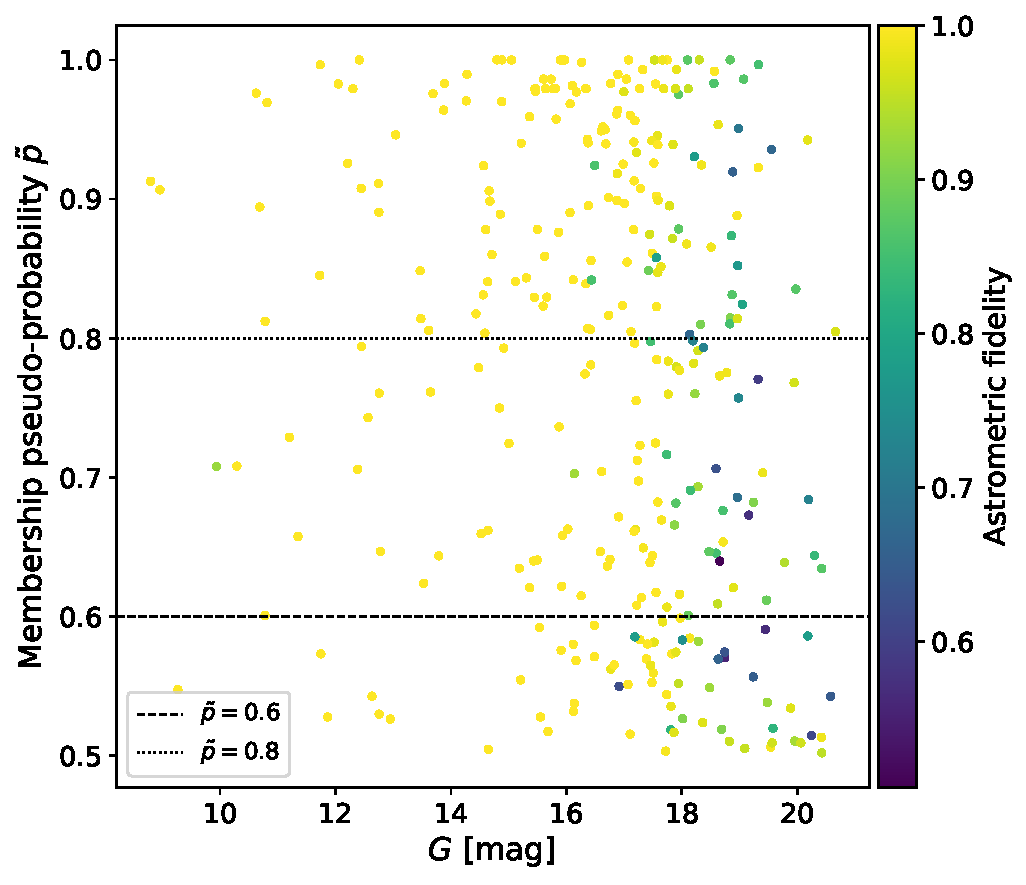
\includegraphics{Figures/probabilies_post_sigmaclip.pdf}}
		\caption{Membership pseudo-probability $\tilde{p}$ of potential NGC 6383 members ($\tilde{p}>0.5$) against their $G$ magnitudes; each point is a star, color-coded by astrometric fidelity. The horizontal dashed and dotted lines, at $\tilde{p}=0.6$ and $\tilde{p}=0.8$ respectively, mark the thresholds used to distinguish between probable members ($0.6\leq\tilde{p}<0.8$) and members ($\tilde{p}\geq0.8$) of the cluster.}
	\label{fig:probabilities}
\end{figure}

Regarding membership pseudo-probabilities (Fig. \ref{fig:probabilities}), NGC 6383 has $321$, $254$, $202$, and $161$ candidate members with $\tilde{p}$ above $50$, $60$, $70$, and $80$\%, respectively. Correspondingly, $288$, $236$, $191$, and $153$ of these candidates are brighter than $G=19\,\mathrm{mag}$. Table \ref{tab:cds_members} shows a five-row excerpt of the likely-member catalog; the complete 321-source catalog is available at the CDS (see Data availability), with the full column set listed in the table note and the CDS ReadMe.

The cone-search robustness experiment (Appendix \ref{app:window}, Table \ref{tab:cone_robustness}) shows how this selection behaves when the input field is widened; the corresponding astrometric and King-structural parameters recovered at each radius are compiled in Table \ref{tab:cone_params}. The NGC 6383-like proper-motion branch is recovered in every run, but the recovered reference sample is not invariant with radius. In the $40$ and $50\,\mathrm{arcmin}$ runs the generic sweep-selected branch coincides with the NGC-like branch. In the $60$ and $70\,\mathrm{arcmin}$ runs, however, the generic branch selected by the sweep differs from the branch closest to the NGC 6383 proper-motion overdensity, showing that the automated branch selection becomes field-window dependent in larger cones.

At the catalog level the solution is stable: the $50\,\mathrm{arcmin}$ run, in which the automated sweep selects the same branch as the NGC-like criterion, returns mean parallax, mean proper motions, and refitted King parameters consistent with the adopted values (Table~\ref{tab:cone_params}). At $60$ and $70\,\mathrm{arcmin}$, where the sweep-selected branch diverges from the NGC-like branch and the $\tilde{p}\geq0.6$ sample inflates to $443$ and $628$ sources, the solution degrades coherently: the proper-motion dispersions grow and the means drift (Table~\ref{tab:cone_params}), and the refitted profile reflects the added contamination through a smaller $R_c$, while the outer radius, now background-constrained, reaches $54^{+7}_{-11}\,\mathrm{arcmin}$ (Sect.~\ref{subsec:structural}, Appendix~\ref{app:window}).

At the source level, the runs agree well: the wider fields recover $203$ ($80\%$), $242$ ($95\%$), and $252$ ($99\%$) of the adopted $254$ at $50$, $60$, and $70\,\mathrm{arcmin}$, and $192$ sources ($76\%$) appear in all four runs. The $50\,\mathrm{arcmin}$ run adds only $33$ sources, all but one beyond the $40\,\mathrm{arcmin}$ footprint. The $60$ and $70\,\mathrm{arcmin}$ runs, by contrast, add $201$ and $376$ sources, of which $83$ and $114$ lie \emph{inside} the $40\,\mathrm{arcmin}$ footprint, the signature of a lowered effective selection threshold rather than of newly resolved outer structures. This behavior is consistent with increasing field contamination, although distinguishing contaminants from genuinely extended populations would require additional photometric, dynamical, or three-dimensional diagnostics (Sect.~\ref{subsec:structural}). We therefore use the $40\,\mathrm{arcmin}$ catalog as the reference membership sample, and the wider extractions to constrain the outer structure (Sect.~\ref{subsec:structural}), while treating the outer membership and any quantity tied to the cluster boundary as search-window sensitive.

\begin{table*}
\caption{Excerpt of the likely-member catalog for NGC 6383. The complete machine-readable table is available at the CDS.}
\label{tab:cds_members}
\centering
\resizebox{\hsize}{!}{%
\begin{tabular}{llllllll}
\hline\hline
GaiaDR3 & RAdeg & DEdeg & Gmag & pHDBSCAN & pFreq & pMember & Ref \\
 & (deg) & (deg) & (mag) & & & & \\
\hline
4053793547964747904 & 264.16939344 & -33.03325935 & 17.9052 & 0.7959 & 0.9793 & 0.7795 & 1 \\
4054500465190725632 & 263.10710918 & -32.96962071 & 20.1954 & 0.6985 & 0.9793 & 0.6840 & 1 \\
4054501599068361216 & 263.08486813 & -32.91805440 & 15.1189 & 0.8585 & 0.9793 & 0.8407 & 1 \\
4054514449600386304 & 263.64147648 & -33.22555846 & 16.3805 & 0.9110 & 0.9828 & 0.8953 & 1 \\
4054518023012382592 & 264.01601176 & -33.15455344 & 14.6423 & 0.6760 & 0.9793 & 0.6620 & 1 \\
\hline
\end{tabular}}
\tablefoot{The complete CDS table contains the following columns: GaiaDR3, RAdeg, DEdeg, Plx, e\_Plx, pmRA, e\_pmRA, pmDE, e\_pmDE, Gmag, BPmag, RPmag, Jmag, Hmag, Ksmag, Fidelity, pHDBSCAN, pFreq, pMember, Ref, PMSProb, AvSag, and logAgeSag. Here pMember is the composite membership pseudo-probability $\tilde{p}=p_{\mathrm{HDBSCAN}}f_i$. The column Ref is equal to one for sources belonging to the $\tilde{p}\geq0.6$ reference sample used for the main cluster parameters, and zero otherwise.}
\end{table*}

\section{Astrometric parameters}\label{sec:astrometry}
\subsection{Parallax and distance}\label{subsubsec:parallax}
Distance estimation from parallax is challenging due to measurement errors, making the conversion from parallax to distance via the simple inverse method unreliable \citep{2015PASP..127..994B,2021AJ....161..147B}. Choosing an appropriate prior distribution is crucial. To address this challenge, we obtained photo-geometric and geometric distances from \citet{2021AJ....161..147B}, who introduced a Bayesian approach incorporating a prior distribution tailored to different regions of the sky, improving distance estimates from \textit{Gaia} EDR3 data. However, we opted not to use photogeometric distances due to the presence of PMS stars and gas in the cluster, which could distort the magnitudes and colors.

When analyzing the parallax measurements of stars within an open cluster, and assuming a simplified one-dimensional perspective, we assume that the parallax values follow a normal distribution, $\varpi_i \sim \mathcal{N}(\mu_\varpi,\sigma_\varpi)$, where $\mathcal{N}(\mu,\sigma)$ denotes a normal distribution with mean $\mu$ and standard deviation $\sigma$. The mean was given a uniform prior, $\mu_\varpi \sim \mathcal{U}(0.5\,\bar{\varpi},\,1.5\,\bar{\varpi})$, where $\mathcal{U}(a,b)$ denotes the uniform distribution on the interval $[a,b]$ and $\bar{\varpi}$ is the arithmetic mean of the observed parallaxes of the sources entering the fit (those with fractional parallax error below $0.1$; see below). The dispersion was given a half-normal prior, $\sigma_\varpi \sim \mathcal{HN}(s_\varpi)$, where $\mathcal{HN}(s)$ denotes the half-normal distribution with scale $s$ and $s_\varpi$ is the standard deviation of the same observed parallaxes. We use the $\mathcal{N}$, $\mathcal{U}$, and $\mathcal{HN}$ notation for all priors in the remainder of the paper. Additionally, we assume a gamma distribution for the distances, parameterized by its mean $\mu_r$ and width $\sigma_r$, the latter with a half-normal prior, $\sigma_r \sim \mathcal{HN}(s_r)$, with $s_r$ the standard deviation of the geometric distances introduced above.

In our hierarchical model, we calculate the mean $(\mu_{\mathrm{prior}})$ between the frequentist average distance derived from parallaxes and the \citet{2021AJ....161..147B} geometric distances, using $\mathcal{U}(0.5\mu_{\mathrm{prior}},1.5\mu_{\mathrm{prior}})$ as the prior for the cluster's mean distance. Our analysis is limited to sources with a fractional parallax error below $0.1$, i.e. $\delta\varpi/\varpi<0.1$ where $\delta\varpi$ is the \textit{Gaia} parallax uncertainty, to ensure accuracy.

The mean parallax of the subsample used for the distance estimate is $0.908\,\mathrm{mas}$, with a 1$\sigma$ dispersion of $0.046\,\mathrm{mas}$ and a standard error on the mean of $0.004\,\mathrm{mas}$ (Fig. \ref{fig:parallax_distance}). The mode sampled distance is $1.11 \pm 0.06\,\mathrm{kpc}$. These values slightly deviate from the results obtained in earlier studies \citep{1930LicOB..14..154T,1949ApJ...110..117S,1978MNRAS.182..607F,1985AA...151..391T,2007AA...462..157P} but agree with \citet{1971AAS....4..241B} and with later determinations \citep{2005AA...438.1163K,2008AA...477..165P,2021ApJ...923..129J,2022ApJS..262....7H,2024arXiv240301030P,2024arXiv240305143H}.

\begin{figure*}
	\centering
	\resizebox{\hsize}{!}{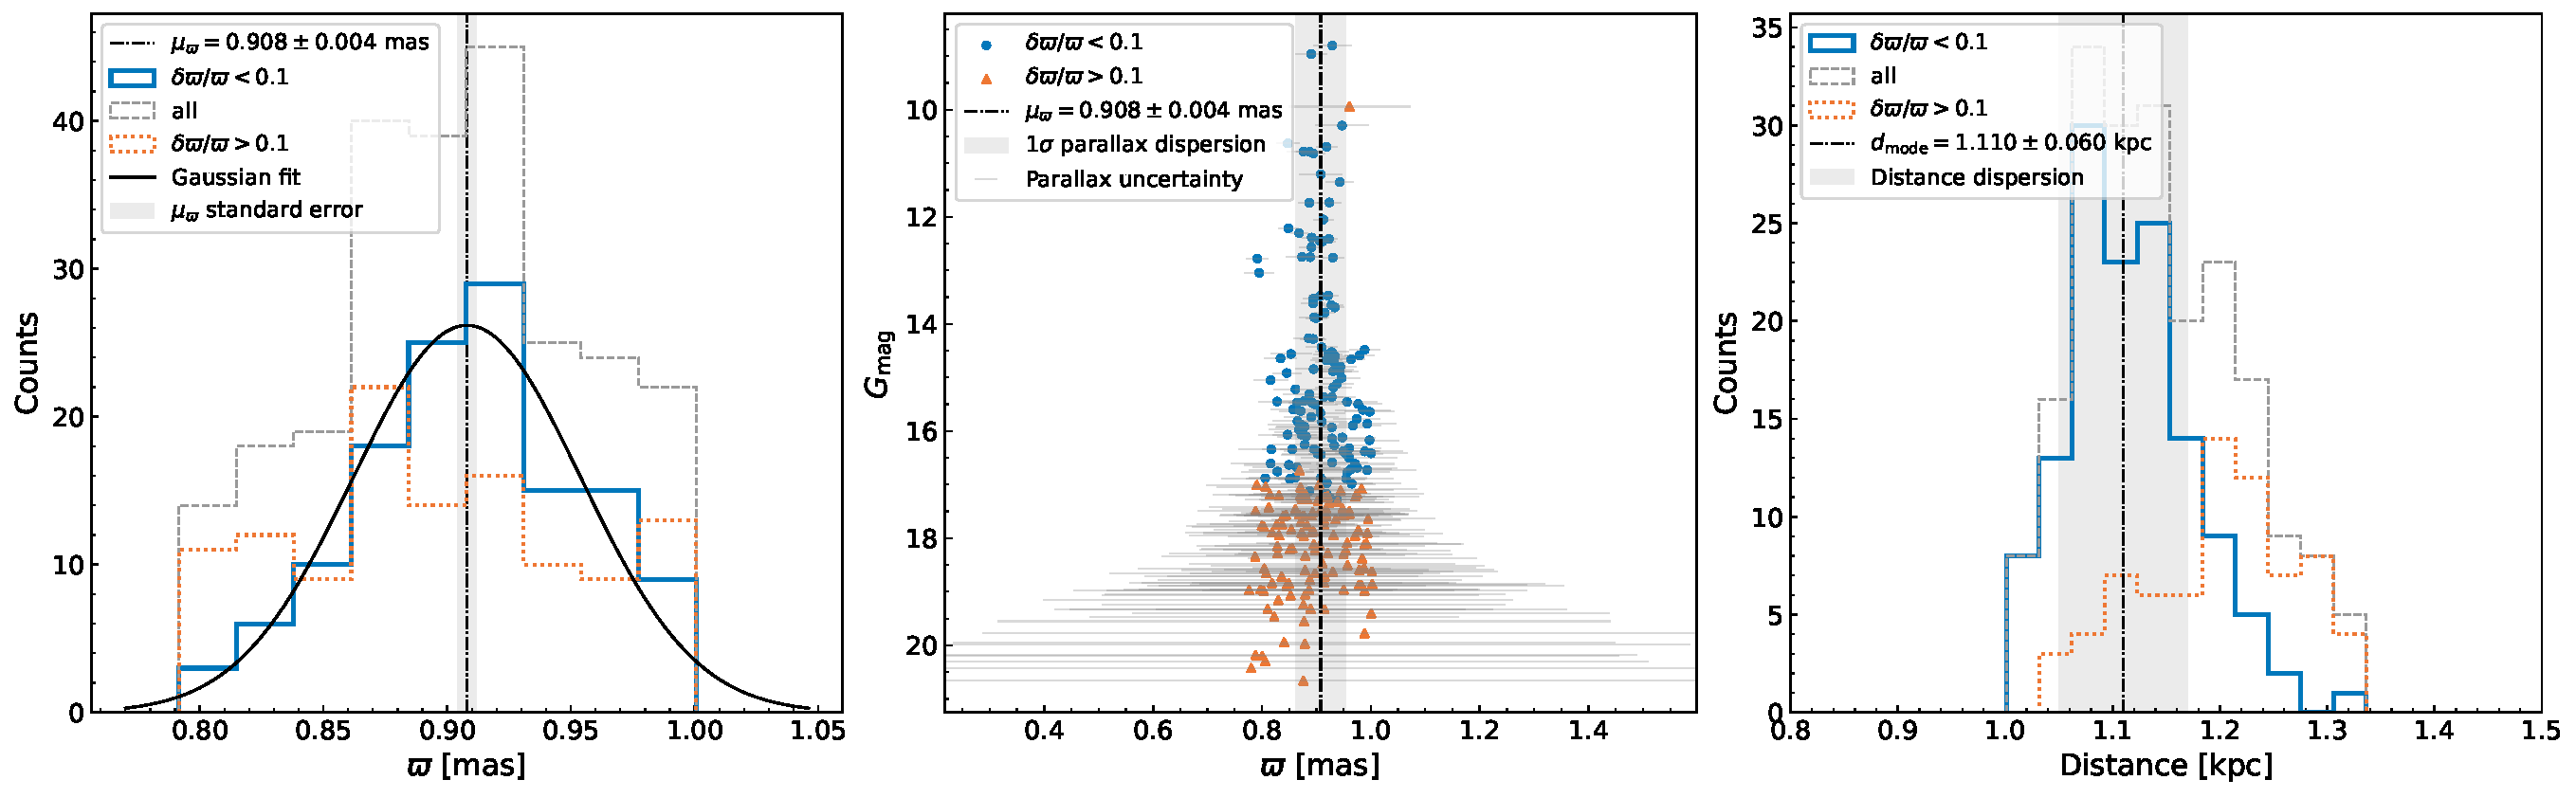
\includegraphics{Figures/parallax_determination_paper.pdf}}
	\caption{\emph{Left panel:} Parallax distribution of the 254-source reference sample, split by fractional parallax error into the subsample used for the estimate ($\delta\varpi/\varpi<0.1$), all sources, and the discarded $\delta\varpi/\varpi>0.1$ sources; the smooth curve is a Gaussian fit, and the dash-dotted line and shaded band mark the mean parallax and its standard error. \emph{Middle panel:} $G$ magnitude versus parallax with the same split; horizontal bars are the individual parallax uncertainties and the shaded band the $1\sigma$ parallax dispersion. \emph{Right panel:} Bailer-Jones geometric distances \citep{2021AJ....161..147B} with the same split; the dash-dotted line and shaded band mark the adopted distance (the mode of the sampled distances) and its dispersion. Values are given in the panel legends. For convenience, only the portion of the histogram corresponding to distances within $0.8$ to $1.2$ times the minimum and maximum used distances is displayed.}
    \label{fig:parallax_distance}
\end{figure*}

\subsection{Proper motions and radial velocities}\label{subsec:pmrv}
We used a two-dimensional Gaussian to model the distribution of the proper motions of the cluster members. A normal prior distribution was assigned to the mean proper motions $\left[\overline{\mu_\alpha},\overline{\mu_\delta}\right]$, based on frequentist means and standard deviations. For the standard deviations, we used half-normal priors with a width equal to the frequentist standard deviation of the proper motions, and the correlation coefficient between the proper motions was uniformly distributed over the interval $[-1, 1]$. Additionally, we estimated the mean total proper motion of the cluster, defined as the quadrature sum of the proper-motion components.

The mean proper-motion values are $2.542\,\mathrm{mas\,yr^{-1}}$ in R.A. and $-1.713\,\mathrm{mas\,yr^{-1}}$ in Dec., with member dispersions of $0.152$ and $0.138\,\mathrm{mas\,yr^{-1}}$, respectively, which align with the acceptable values from \citet{2023MNRAS.526.4107P} (Fig. \ref{fig:proper_motion}). The corresponding standard errors on the means are $0.0096$ and $0.0086\,\mathrm{mas\,yr^{-1}}$, but these smaller values are not used as the physical width of the cluster when comparing individual stars. The posterior distribution of the total proper motion, derived as the quadrature sum of the two components in each draw, has a median of $3.065 \pm 0.009\,\mathrm{mas\,yr^{-1}}$, corresponding to a projected (tangential) velocity of $16.1 \pm 0.9\,\mathrm{km\,s^{-1}}$ at the adopted distance.

The dispersions quoted above are those of the observed member sample and therefore still contain the \textit{Gaia} measurement scatter. Because the per-source proper-motion uncertainties of the members span two orders of magnitude (median $0.104$ and $0.074\,\mathrm{mas\,yr^{-1}}$ in $\mu_{\alpha*}$ and $\mu_\delta$, with $32\%$ and $23\%$ of members having uncertainties larger than the observed scatter itself), subtracting a mean error in quadrature is not defined here: it returns a negative variance in both axes. We therefore estimated the intrinsic dispersion by maximum likelihood, modeling each member as $\mu_i \sim \mathcal{N}(\overline{\mu}, \sigma_{\mathrm{int}}^2 + e_i^2)$ with its own uncertainty $e_i$, which gives $\sigma_{\mathrm{int}} = 0.122$ and $0.121\,\mathrm{mas\,yr^{-1}}$ in $\mu_{\alpha*}$ and $\mu_\delta$, that is a one-dimensional intrinsic dispersion of $0.122\,\mathrm{mas\,yr^{-1}}$, or $0.64\,\mathrm{km\,s^{-1}}$ at the adopted distance. The apparent excess of the R.A. over the Dec. dispersion (a ratio of $1.11$ in the observed values) disappears after this deconvolution (a ratio of $1.00$), showing it to be an artifact of the \textit{Gaia} error budget, which is larger in $\mu_{\alpha*}$, rather than a kinematic anisotropy. The intrinsic value is more sensitive to the membership selection than to the fit: repeating the estimate at $\tilde{p}\geq0.5$, $0.7$, and $0.8$ gives $0.150$, $0.102$, and $0.089\,\mathrm{mas\,yr^{-1}}$, a monotonic trend that reflects the progressive truncation of the member sample in proper-motion space rather than a symmetric uncertainty, so we treat this quantity as selection-limited. We retain the observed dispersions in Table~\ref{tab:ngc6383_results} and in the individual-star comparisons below, because they are the appropriate width against which to ask whether a single star is an outlier of the observed member population, and quote the intrinsic value here only for comparison with dynamical work.

\textit{Gaia} DR3 radial velocities are available for only $11.4$\% of the reference sample (29 of 254 sources). Because sources with large radial-velocity amplitudes, likely unresolved binaries, can bias the cluster's radial-velocity estimate, we restricted it to the 16 clustered sources with $\tilde{p}\geq0.6$ and a binary probability (an ASteCA product; Sect.~\ref{subsec:lum_mass_dyn}) lower than $0.6$. The resulting median, mean, and standard deviation are $-1.87$, $-9.40$, and $32.1\,\mathrm{km\,s^{-1}}$, respectively. The substantial standard deviation primarily stems from the limited availability of radial velocity data, and even with the binary cut the small sample makes this only an indicative measure of the cluster's internal dynamics. Figure \ref{fig:radial_velocities} illustrates all the probable members and members with available radial velocities, their magnitudes, and the amplitude of their radial velocities.

\begin{figure}
	\centering
	\resizebox{\hsize}{!}{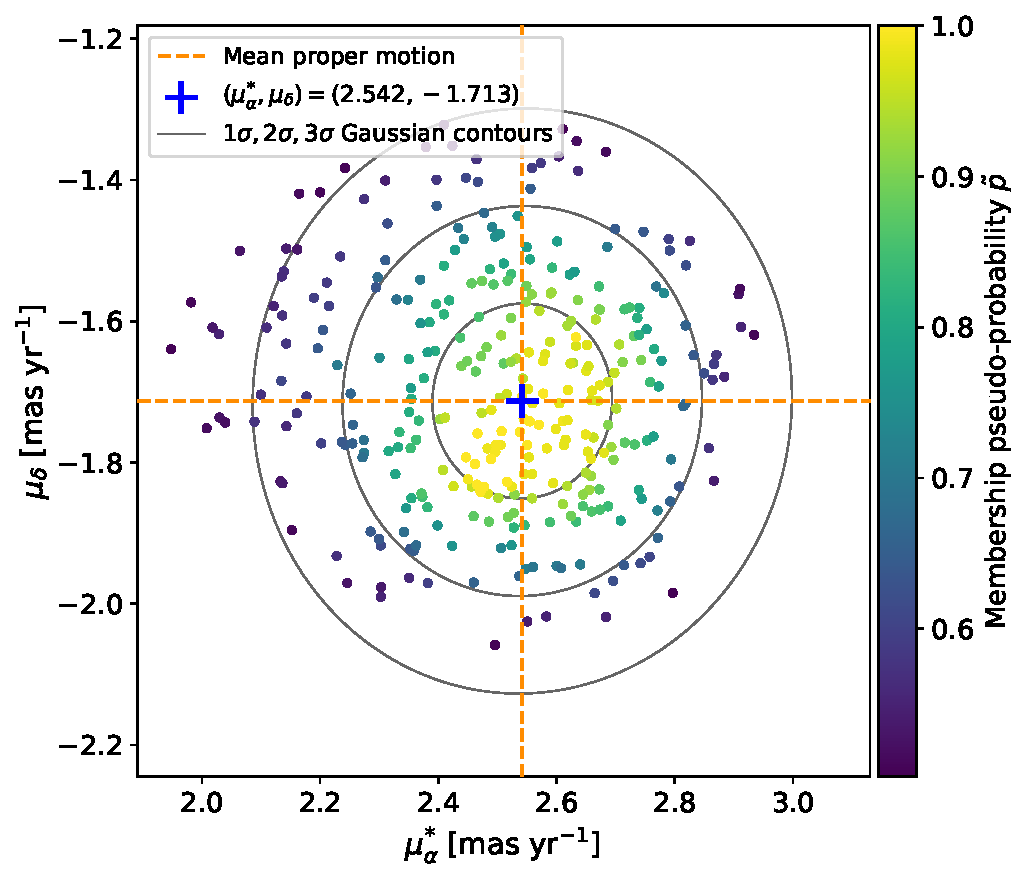
\includegraphics{Figures/proper_motion_2d_paper.pdf}}
	\caption{Proper motions of the likely cluster candidates ($\tilde{p}>0.5$) of NGC 6383; the symbols are color-coded according to the membership pseudo-probability $\tilde{p}$ of the stars. The gray solid ellipses are the 1$\sigma$, 2$\sigma$, and 3$\sigma$ iso-probability contours of the two-dimensional Gaussian proper-motion model fitted to the reference sample. The inferred mean proper motion is marked with a blue cross and with the orange dashed lines through it.}
	\label{fig:proper_motion}
\end{figure}

\subsection{Cluster center}\label{subsec:center}
To determine the cluster's center, we used a weighted Kernel Density Estimation (KDE) from the Python library \textsc{scikit-learn} \citep{scikit-learn}, assigning weights inversely proportional to the distance from the mean proper motion. Optimal KDE parameters were determined through Grid Search Cross-Validation within the package, exploring a range of bandwidths (from the mean positional error to the cone-search radius) and all kernel types; the selected bandwidth ($\approx6.7\,\mathrm{arcmin}$) dominates the quoted center uncertainty. The location of maximum density was taken as the cluster's center.

The central position of the cluster in equatorial coordinates is $263.683 \pm 0.112\,^\circ$ in R.A. and $-32.584 \pm 0.112\,^\circ$ in Dec. (Fig. \ref{fig:center}). These errors are calculated from the quadratic sum of the mean errors in R.A. and Dec., and the optimal KDE bandwidth. This center is consistent, within the quoted uncertainty, with the projected coordinates of HD 159176; the positional coincidence is therefore not sufficient by itself to establish membership.

\begin{figure}
	\centering
	\resizebox{\hsize}{!}{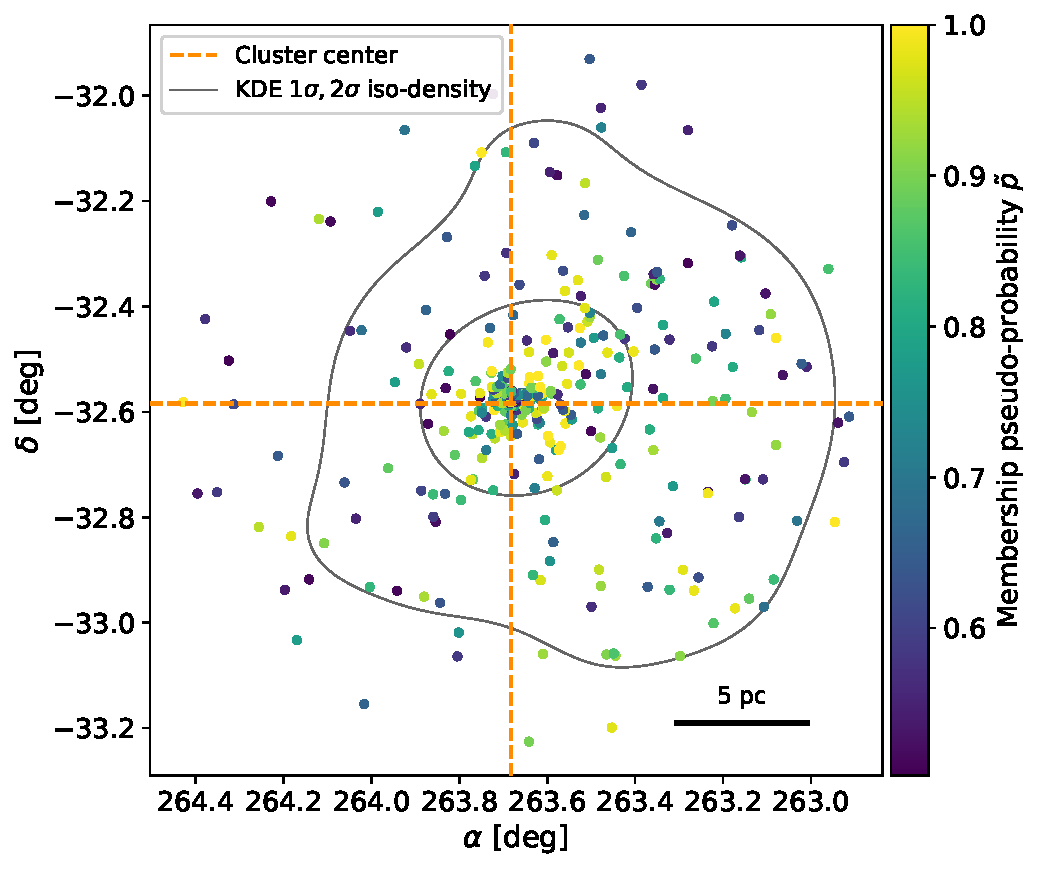
\includegraphics{Figures/center_determination_paper.pdf}}
		\caption{Spatial distribution of the likely cluster candidates ($\tilde{p}>0.5$) of NGC 6383 in right ascension ($\alpha$) and declination ($\delta$), color-coded according to their membership pseudo-probability $\tilde{p}$. The gray solid contours are the 1$\sigma$ and 2$\sigma$ iso-density contours (enclosing $39\%$ and $86\%$) of a kernel density estimate of the candidate positions, revealing the density gradient of the points. The central coordinates of the cluster are marked by dark-orange dashed lines, which approximately coincide with the density peak within the plotted area.}
	\label{fig:center}
\end{figure}

\section{Cluster structure}\label{subsec:structural}
To determine the structural parameters of the cluster, we utilized the \citet{1962AJ.....67..471K} density profile. The numerical density $\rho$ was computed by dividing the cluster area into concentric annuli, each containing an equal number of stars. The number of annuli, $K$, adheres to the equiprobable bin rule ($K = 2n^{2/5}$), where $n$ is the star count within the cluster. The annular densities were fit with a Gaussian likelihood whose scatter is a half-normal nuisance parameter, yielding the posterior distribution of the structural parameters.

Priors for the model parameters were set as follows: $b \sim \mathcal{U}(0, 2\rho_{\mathrm{min}})$, $k \sim \mathcal{U}(b, 2\rho_{\mathrm{max}})$, $R_c \sim \mathcal{U}(0, 0.8\,T_{\mathrm{max}})$, and $R_t \sim \mathcal{U}(R_c, 1.5\,T_{\mathrm{max}})$, where $b$ is the background density, $k$ the central normalization, $\rho_{\mathrm{min}}$ and $\rho_{\mathrm{max}}$ the observed surface-density extrema, and $T_{\mathrm{max}}$ the highest value between the Hill radius and the gravitational bound radius, both defined below. These coefficients are not tuned values but weakly informative bounds anchored to the largest physically meaningful scale of the system. The upper limit on $R_c$ lies more than an order of magnitude above any realistic open-cluster core radius. The upper limit on $R_t$ allows the fitted outer radius to exceed the nominal gravitational bound radius by up to $50\%$, generous headroom for the uncertainties in the cluster mass and Galactic potential that enter $T_{\mathrm{max}}$.

The posterior of $R_c$ is confined well inside its support (97.5th percentile at $\simeq2.5\,\mathrm{arcmin}$, $7\%$ of the prior upper bound), so its bound is immaterial. Refitting the $40\,\mathrm{arcmin}$ profile with alternative coefficients (e.g., $0.9\,T_{\mathrm{max}}$ and $1.2\,T_{\mathrm{max}}$) changes $R_c$, $k$, $b$, and $C$ by less than $0.5\sigma$; only the weakly constrained outer radius responds (median $R_t\simeq33\,\mathrm{arcmin}$ versus $40^{+16}_{-17}\,\mathrm{arcmin}$, consistent within $1\sigma$). For the adopted $70\,\mathrm{arcmin}$ fit the same coefficients act differently, and the arithmetic is worth stating: with $T_{\mathrm{max}}=42.5\,\mathrm{arcmin}$, a bound of $1.2\,T_{\mathrm{max}}=51.0\,\mathrm{arcmin}$ lies \emph{below} the adopted $R_t=54\,\mathrm{arcmin}$, so any coefficient smaller than $1.27$ excludes the adopted value from the prior support outright rather than perturbing it. This is not an independent objection to that value but the same prior limitation seen from the opposite side: $R_t$ is bounded from above by the prior in every window we fit, which is why we report it as conditional on the bound and quantify the relaxed case below. The outer radius is the one parameter whose posterior is sensitive to the prior support in all windows: the upper bound $1.5\,T_{\mathrm{max}}=63.7\,\mathrm{arcmin}$ truncates the $R_t$ posterior of every fit. All quoted $R_t$ intervals are therefore conditional on this physically motivated prior (Appendix~\ref{app:window}), reinforcing its interpretation as a model-dependent outer scale.

The Hill radius $(R_\mathrm{Hill})$, which defines the region around a star cluster where its gravitational influence dominates over that of the Galaxy, can be calculated following \citet{2019A&A...627A.119C}:
\begin{equation}
R_\mathrm{Hill} = R_{\mathrm{gc}} \times \left(\frac{m_c}{3M_{\mathrm{gc}}}\right)^{1/3}
\end{equation}
where $R_{\mathrm{gc}} = \left(R_\odot^{2} + d^{2} - 2 R_\odot d \cos l \cos b\right)^{1/2} = 7.19 \pm 0.06\,\mathrm{kpc}$ is the galactocentric distance of the cluster, computed from its Galactic coordinates $(l,b)$, the parallax-based distance $d = 1.11 \pm 0.06\,\mathrm{kpc}$, and a solar galactocentric radius $R_\odot = 8.3\,\mathrm{kpc}$ \citep{2016ApJS..227....5D}, with the uncertainty propagated from the distance and cluster-center uncertainties, $ m_c $ the cluster mass from \citet{2024arXiv240305143H}, with a value of $902 \pm 92~M_\odot$, and $ M_{\mathrm{gc}} $ the Galactic mass enclosed within the cluster's orbit, estimated from the circular velocity of the \citet{2017MNRAS.465...76M} Galactic potential at $R_{\mathrm{gc}}$, $V_c(7.19\,\mathrm{kpc}) \simeq 229\,\mathrm{km\,s^{-1}}$, as
\begin{equation}
	M_{\mathrm{gc}} = \frac{V_c^2(R_{\mathrm{gc}})\, R_{\mathrm{gc}}}{G} = (8.8 \pm 0.5) \times 10^{10}\,M_\odot,
\end{equation}

Moreover, the gravitationally bound radius was estimated using the method described by \citet{1998MNRAS.299..955P}, which considers the cluster mass and Oort constants, using the formula
\begin{equation}
	r_\mathrm{bound} = \left( \frac{Gm_{\mathrm{c}}}{2(A-B)^2} \right)^{1/3},
\end{equation}
where $G$ is the gravitational constant, and $A$ and $B$ are the Oort constants, with values from \citet{2017MNRAS.468L..63B}.

The King fit to the $40\,\mathrm{arcmin}$ reference sample yields a core radius $R_c = 1.96^{+0.19}_{-0.16}\,\mathrm{arcmin}$ ($0.63^{+0.06}_{-0.05}\,\mathrm{pc}$), with $k = 4.92^{+0.43}_{-0.31}$ and background $b = 0.011\pm0.007$ stars per square arcminute (Fig.~\ref{fig:king}). The outer radius, however, is not usefully constrained by this window: the fit returns $R_t = 40^{+16}_{-17}\,\mathrm{arcmin}$ with half of the posterior mass beyond the extraction radius itself, because the field contains almost no background annulus beyond the cluster.

We therefore measure the outer structure on the wider extractions of Appendix~\ref{app:window}, refitted with identical priors. The fitted $R_t$ is mutually consistent across all windows (Table~\ref{tab:cone_params}), and the $70\,\mathrm{arcmin}$ window is the only one whose radial profile reaches a fitted background annulus beyond the cluster (Fig.~\ref{fig:king70}). We adopt $R_t = 54^{+7}_{-11}\,\mathrm{arcmin}$ ($17.4^{+2.3}_{-3.6}\,\mathrm{pc}$) as the King outer radius. This interval remains conditional on the $R_t<1.5\,T_{\mathrm{max}}=63.7\,\mathrm{arcmin}$ prior: relaxing the bound to the extraction edge ($R_t<70\,\mathrm{arcmin}$) shifts the posterior to $58^{+9}_{-13}\,\mathrm{arcmin}$, consistent within $1\sigma$, with the upper tail still limited by the prior support rather than turned over by the data. The wider windows also admit additional field contamination in the membership (Sect.~\ref{subsec:member_results}), which lowers the fitted $R_c$ to $\simeq1.4\,\mathrm{arcmin}$ at $60$--$70\,\mathrm{arcmin}$; the selection-stable $50\,\mathrm{arcmin}$ run returns $R_c = 1.90^{+0.15}_{-0.13}\,\mathrm{arcmin}$, confirming the adopted core radius. Combining the adopted $R_c$ and $R_t$ posteriors gives a concentration parameter $C = \log_{10}(R_t/R_c) = 1.43^{+0.07}_{-0.10}$ \citep{1975AJ.....80..427P}. Because the added outer sources cannot be separated from field contamination without additional diagnostics \citep{2025A&A...694A.258R,2025A&A...698A.156X}, $R_t$ remains a model-dependent scale rather than a sharp physical boundary. All the radii quoted here come from a circularly symmetric fit; no axis ratio was fitted, so $R_c$ should be read as the geometric-mean scale radius of the projected distribution rather than as a semi-major axis. The half-light radius is determined to be $6.02 \pm 1.07\,\mathrm{arcmin}$ ($1.94 \pm 0.36\,\mathrm{pc}$, bootstrap uncertainty) and the half-mass radius is $6.26 \pm 1.23\,\mathrm{arcmin}$ $(2.02 \pm 0.41\,\mathrm{pc})$.

Measuring the outer structure on a field substantially larger than the cluster itself follows established \textit{Gaia} DR3 practice \citep{2025MNRAS.539.2513A}; even so, the wider-field tests (Appendix \ref{app:window}, Table \ref{tab:cone_robustness}) show that the number of outer candidates changes with the input field, so we do not classify the larger-radius additions as confirmed halo members or contaminants. We identify $18$ sources beyond the Hill radius ($33.6\,\mathrm{arcmin}$) with cluster-like proper motions (pseudo-probabilities $0.64$--$1.0$, mean $0.81$; Fig. \ref{fig:real_sky}); all lie within the $40\,\mathrm{arcmin}$ extraction, and hence well inside the adopted $R_t$. They also lie inside the gravitational bound radius ($42.5\,\mathrm{arcmin}$); we nevertheless flag them because the Hill radius, which accounts for the Galactic tidal field at the cluster's orbit, is the more conservative boundary of guaranteed boundness, so their membership in the bound system is not certain.

\begin{figure}
	\centering
	\resizebox{\hsize}{!}{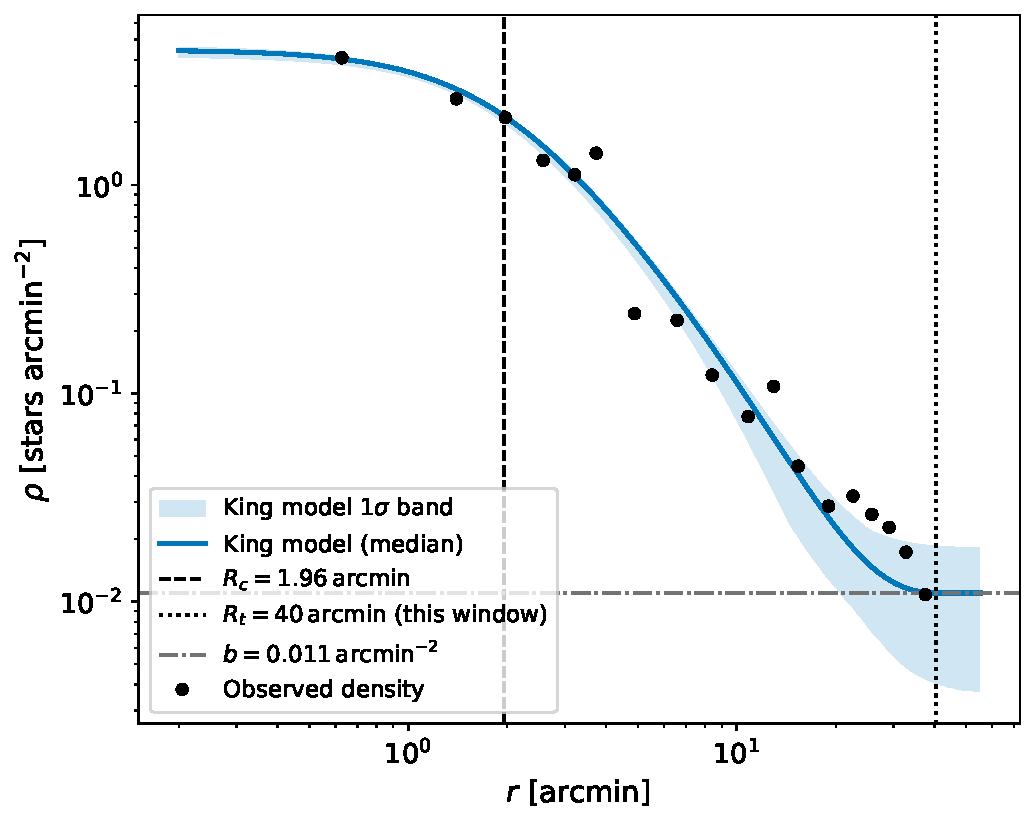
\includegraphics{Figures/king_profile_logscale.pdf}}
	\caption{Radial density profile of NGC 6383 in logarithmic scale: annular number densities of the reference sample with the King model at the posterior median and its 16--84\% posterior band. The vertical lines mark the core radius and the outer radius preferred by this $40\,\mathrm{arcmin}$-window fit, and the horizontal line the fitted background level $b$. The posterior band is narrow near the core, where the profile is set by the well-constrained central density, and broadens markedly at large radii, where this window contains almost no background annulus; the adopted outer radius, $R_t = 54^{+7}_{-11}\,\mathrm{arcmin}$, is measured on the $70\,\mathrm{arcmin}$ extraction (Appendix~\ref{app:window}, Fig.~\ref{fig:king70}).}
	\label{fig:king}
\end{figure}

\section{Age, extinction, and stellar content}\label{sec:stellar}
\subsection{Isochrone fitting with ASteCA}\label{subsec:asteca}
Automated Stellar Cluster Analysis (ASteCA) \citep{2015A&A...576A...6P}, is an open-source Python tool designed to automate standard tests for determining basic parameters of stellar clusters. For accurate estimation of a cluster's metallicity, age, and extinction values, we employed ASteCA's isochrone fitting process. We utilized the \textsc{MIST} isochrones \citep{2016ApJS..222....8D, 2016ApJ...823..102C} along with the photometric systems of \textit{Gaia} EDR3 and \textsc{2MASS}. The Initial Mass Function followed \citet{2014ApJ...796...75C}. Synthetic binaries were generated with the mass-dependent binary fraction adopted in ASteCA, $b(m)=\alpha+\beta/(1+1.4/m)$ with $\alpha=0.090$ and $\beta=0.940$ held fixed; this parametrization is ASteCA's analytic fit to the observed multiplicity fraction as a function of primary mass compiled by \citet{2023ASPC..534..275O}, and with these coefficients it reproduces the observed binarity across spectral types, rising from $\simeq0.26$ for M dwarfs through $\simeq0.5$ for solar-type stars to $\gtrsim0.9$ for O-type stars \citep{2013ARA&A..51..269D,2017ApJS..230...15M}. Secondary masses were drawn from the mass-ratio distribution $f(q)\propto q^{\gamma}$ with the mass-dependent exponents of \citet{2013ARA&A..51..269D}; differential reddening was fixed to zero.

The \textsc{MIST} ages inherit the physical assumptions of the underlying models: we used the v1.2 grids, which adopt solar-scaled abundances on the \citet{2009ARA&A..47..481A} scale ($Z_\odot\simeq0.0142$), a single solar-calibrated mixing-length parameter ($\alpha_{\mathrm{MLT}}=1.82$), exponentially decaying convective overshooting ($f_{\mathrm{ov,core}}=0.016$, $f_{\mathrm{ov,env}}=0.0174$), and an initial rotation of $v/v_{\mathrm{crit}}=0.4$ imposed at the zero-age main sequence, so the PMS tracks that dominate our fit are effectively non-rotating. The models include neither magnetic inhibition of convection, nor starspots, nor an accretion history; magnetic and spotted PMS models yield systematically older ages for young clusters, by a factor of $\sim2$ or more \citep{2016A&A...593A..99F,2015ApJ...807..174S}, with the SPOTS grids showing the same systematic \citep{2020ApJ...891...29S}, so the absolute PMS age scale is tied to these assumptions.

The priors for metallicity $Z$, logarithmic age, and absorption $A_V$ were defined as uniform distributions ranging from $[0.001, 0.045]$, $[6.00, 7.00]$, and $[0.5, 2]$, respectively, aligned with the findings of \cite{2024arXiv240301030P}. The distance modulus was modeled as $\mathcal{N}(10.3, 0.2)$, with the mean value corresponding to the expected distance modulus obtained from the parallax. We used only the \textsc{MIST} PMS evolutionary models for the present fit; the fitted spread therefore describes the uncertainty within this model family alone, and the systematic differences that arise from alternative PMS tracks are added separately when the adopted age interval is quoted below. We adopted the mode of the fitted distribution for our analysis and sampled the model with the gradient-free DEMetropolis ensemble sampler (Sect.~\ref{subsec:cosmic}) instead of the Approximate Bayesian Computation (ABC) suggested by ASteCA. The nuisance parameter $\sigma$ shown in the corner plot (Fig.~\ref{fig:plot_pair_trace}) is the likelihood-scatter term of the fit; it is not a physical velocity, spatial, or age dispersion of the cluster.

To determine the cluster's age, extinction, and metallicity, we fit MIST isochrones to the CMD of NGC 6383 (Fig. \ref{fig:cmd}, which shows the PMS stars and the mode, mean, and median isochrones). The mode indicates a logarithmic age in years of $6.55$, a distance modulus of $10.30\pm 0.09\,\mathrm{mag}$ corresponding to a distance of $1.15\pm0.05\,\mathrm{kpc}$, and a metallicity $Z $ of $0.024 \pm 0.008$, slightly above the MIST solar value ($Z_\odot\simeq0.0142$); we note that the absolute metallicity is only loosely constrained by the isochrone fit because of the age--metallicity--extinction degeneracy, and the value lies within the adopted prior. An estimated extinction correction of $A_V = 1.24 \pm 0.26$ was applied. This CMD-derived distance is consistent with the parallax-based value of $1.11 \pm 0.06\,\mathrm{kpc}$ (Table \ref{tab:ngc6383_results}), as expected given that the distance-modulus prior was centered on it, and we adopt the parallax value for all structural-radius conversions.

We caution that the age is a weakly constrained quantity and that the width of its posterior is not a measure of the precision of the fit: the marginal retains a substantial fraction of the adopted $\mathcal{U}(6.00,7.00)$ prior width, so its standard deviation ($0.15\,\mathrm{dex}$) is a lower bound on the true uncertainty rather than a statistical error, and we do not quote it as one. Two considerations set the realistic uncertainty, and both act in the same direction, toward older ages. First, the PMS model family: starspots and magnetic inhibition of convection shift isochrone-derived pre-main-sequence ages by factors of $2$--$10$ and $\sim2$ respectively at $3\,\mathrm{Myr}$ \citep{2015ApJ...807..174S,2016A&A...593A..99F}, that is by $0.3$--$1.0\,\mathrm{dex}$, and neither is included in the \textsc{MIST} v1.2 grids used here (Sect.~\ref{subsec:asteca}, above). Second, the independent indicators available for this cluster all lie above the fitted value: the median \textsc{Sagitta} age of the $116$ PMS candidates of the same membership is $\log(\mathrm{age})=6.75$ (Sect.~\ref{subsec:sagitta}), some $0.2\,\mathrm{dex}$ higher, and the isochrones that bracket the observed PMS locus reach $\log(\mathrm{age})=6.80$ (Fig.~\ref{fig:cmd_ngc6383_various}). We therefore adopt $\log(\mathrm{age}\,\mathrm{yr^{-1}}) = 6.55^{+0.40}_{-0.20}$, i.e. $\simeq3.5\,\mathrm{Myr}$ with a factor $\simeq2.5$ of room toward older ages and $\simeq1.6$ toward younger ones. The bar is deliberately asymmetric: no effect identified here or in the literature pushes the age of this cluster younger, whereas several push it older, and the $+0.40\,\mathrm{dex}$ upper bound is the conservative lower half of the range spanned by the PMS systematics quoted above.

The CMD, particularly for sources brighter than $G=12.0\,\mathrm{mag}$, displays a well-defined main sequence. The presence of PMS stars and lower-mass main-sequence stars broadens the lower part of the CMD, complicating the fit of a single isochrone. Figure \ref{fig:cmd_ngc6383_various} presents various isochrones for \textit{Gaia} and 2MASS data, considering ages between $6.20$ and $7.00$ in logarithmic scale and initial metallicities $ Z $ of $0.024$. The isochrones that best bracket the PMS locus approximately correspond to $\log(\mathrm{age})=6.20$--$6.80$, equivalent to about $1.6$--$6.3\,\mathrm{Myr}$, although older isochrones are plotted to show the sensitivity of the fit. Unresolved binaries, differential reddening (fixed to zero in the fit), and accretion variability also broaden the PMS locus \citep{2010ApJ...723..166D}, so this bracketing range should be read as an upper limit on any true age spread.

Figure \ref{fig:cmd_ngc6383_various} also includes color-color diagrams $(G_\mathrm{BP} - G_\mathrm{RP})$ showing a clearer segregation of PMS stars, which tend to be at redder colors, as expected. The joint distribution of the inferred parameters is shown as a plot pair in Fig. \ref{fig:plot_pair_trace}.

\begin{figure}
	\centering
	\resizebox{\hsize}{!}{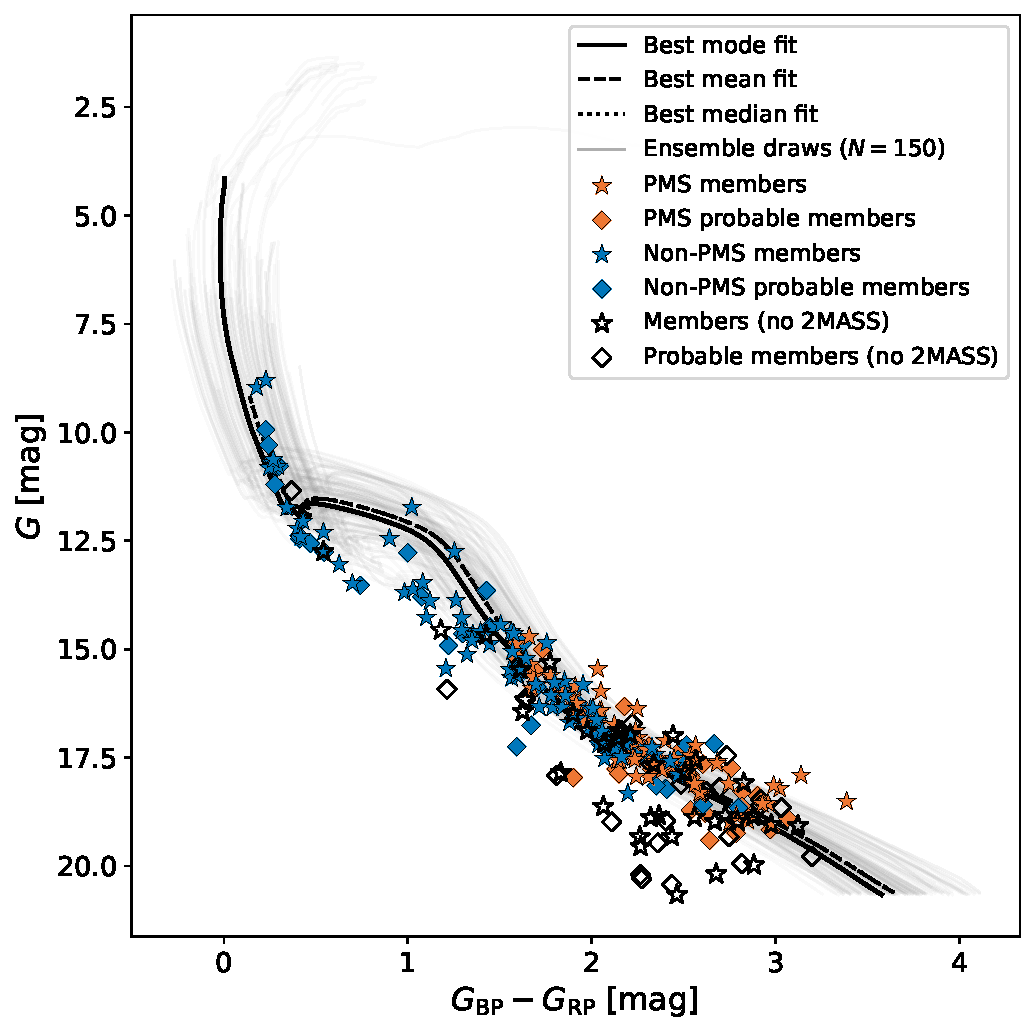
\includegraphics{Figures/ngc6383_cmd.pdf}}
		\caption{CMD of NGC 6383 ($G_{\text{mag}}$ versus $G_{\text{BP}} - G_{\text{RP}}$) with the Sagitta-based PMS classification: orange filled symbols are PMS candidates (Sagitta PMS probability $\geq0.6$), blue filled symbols are non-PMS sources, and open black symbols are sources without 2MASS photometry, which are left unclassified; stars denote members ($\tilde{p}\geq0.8$) and diamonds probable members ($0.6\leq\tilde{p}<0.8$). The black solid, dashed, and dotted curves are the synthetic single-star sequences at the mode, mean, and median of the isochrone-fit ensemble, and the light-gray curves are 150 single-star sequences drawn from that ensemble.}
	\label{fig:cmd}
\end{figure}

\begin{figure*}
	\centering
	\resizebox{\hsize}{!}{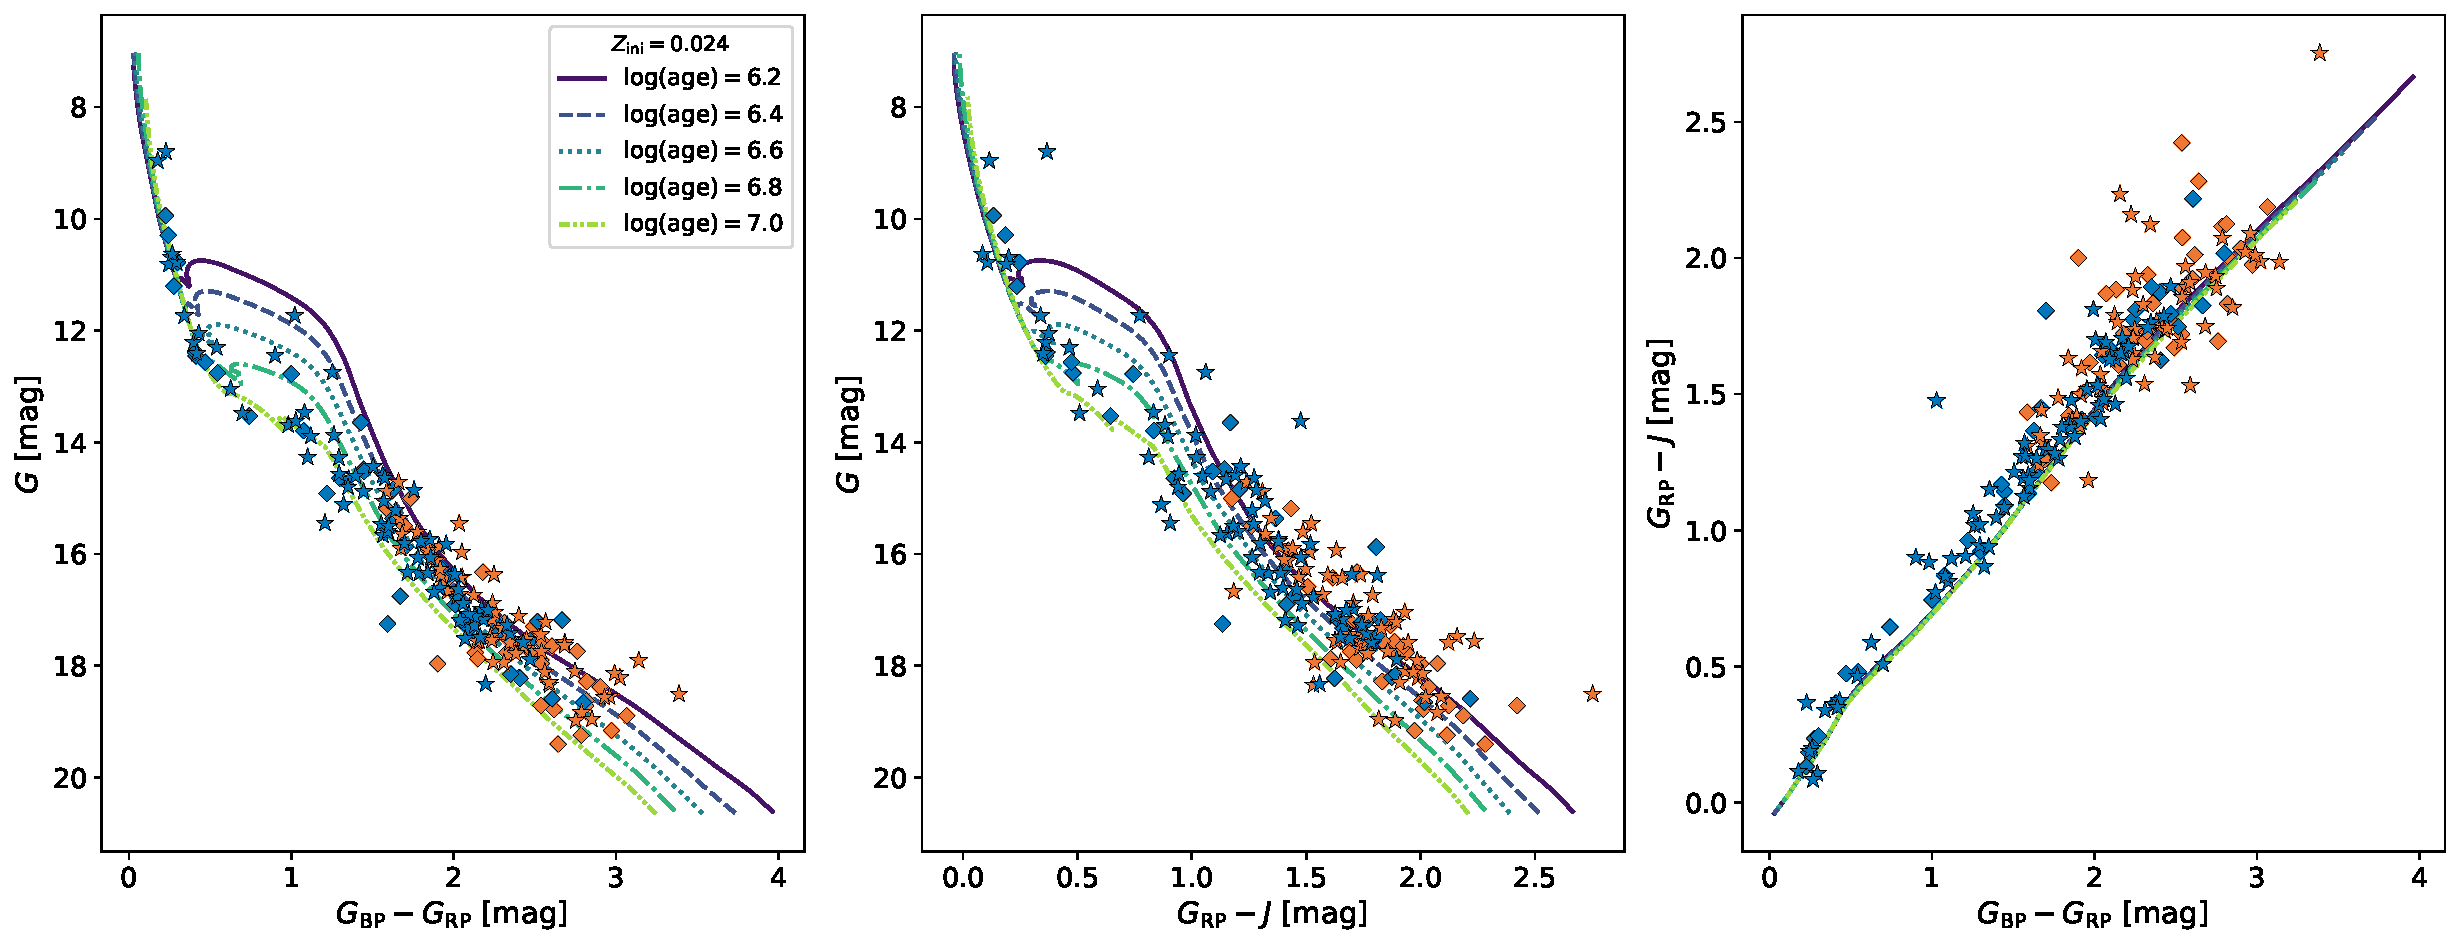
\includegraphics{Figures/ngc6383_cmd_various.pdf}}
	\caption{\emph{Left panel:} CMD of NGC 6383 showing $G_{\text{mag}}$ against $G_{\text{BP}} - G_{\text{RP}}$ with isochrones for $\log(\mathrm{age}~\mathrm{yr}^{-1})$ ranging from $6.20$ to $7.00$. \emph{Middle panel:} CMD using $G_{\text{mag}}$ versus $G_{\text{RP}} - J$. \emph{Right panel:} Color-color diagram, $G_{\text{RP}} - J$ against $G_{\text{BP}} - G_{\text{RP}}$, with the equivalent color-color isochrones. The symbol notation follows that of Fig. \ref{fig:cmd}, representing different member classifications and evolutionary states within NGC 6383. The MIST isochrones for $\log(\mathrm{age})=6.2$--$7.0$ (at $Z_{\text{ini}} = 0.024$) are drawn with sequentially ordered colors and distinct line styles, identified in the left-panel legend, highlighting the evolutionary progression of members within NGC 6383.}
	\label{fig:cmd_ngc6383_various}
\end{figure*}

\subsection{PMS content and YSO fraction}\label{subsec:sagitta}
Sagitta is a neural network designed to classify stars as PMS and estimate their ages. It is trained with data from \textit{Gaia} DR2 and the 2MASS. It incorporates three convolutional neural networks each dedicated to determining stellar extinction ($A_V$), PMS probability, and estimating stellar ages. Sagitta's age estimation is applicable for young stars up to $\sim 80~\mathrm{Myr}$ and relies on inputs including \textit{Gaia} parallaxes, and average line-of-sight extinction \citep{2021AJ....162..282M}.

The tool's efficacy stems from its training on a well-curated dataset of PMS stars within moving groups \citep{2020AJ....160..279K}, which is supplemented by various literature sources with previously measured ages. Sagitta uniquely offers stability in age predictions across G, K, and M-type stars within the same population, surpassing traditional isochrone techniques in consistency \citep{2023AJ....165..182K}. Although the network was trained on \textit{Gaia} DR2 photometry, we apply it to the corresponding \textit{Gaia} DR3 bands.

Identifying PMS stars and estimating their ages traces the cluster's star-formation history. Sagitta is most reliable for PMS stars, as the photometry of higher-mass stars that have reached the main sequence is not indicative of their age, limiting the model's applicability to stars that remain in the PMS stage.

Applying Sagitta to the membership yields $116$ of the $254$ reference-sample sources ($133$ of the $321$ likely candidates) with a PMS probability of at least $0.6$, the threshold used for the PMS class throughout this paper. The distributions of the per-star Sagitta PMS probabilities, ages, and extinctions are shown in Fig.~\ref{fig:pms_sagitta_stats}. These histograms are individual-star Sagitta estimates and should not be read as the same posterior summarized in Table \ref{tab:ngc6383_results}: the broader Sagitta distributions, including the high-extinction tail and older age tail, reflect star-to-star extinction, photometric scatter, unresolved binaries, and the fact that Sagitta is applied to individual PMS candidates, whereas the ASteCA values in Table \ref{tab:ngc6383_results} are cluster-level isochrone-fit parameters.


Young stellar objects (YSOs) are early-stage stars still accreting material from circumstellar disks; they include protostars and the more evolved PMS stars, the latter comprising classical T-Tauri and Herbig Ae/Be stars.

Our analysis aims to quantify the fraction of YSOs within the cluster, noted as $ Y_{\text{frac}} $, which serves as an age indicator. We determined the reddening-free parameter $ Q $ for each star using
\begin{equation}
	Q = (J - H) - \frac{E(J-H)}{E(H - K)} (H-K),
\end{equation}
where $ E(J-H)/E(H-K) $ is assumed to be $1.55$ \citep{1990ARA&A..28...37M}. Following \citet{2013MNRAS.436.1465B}, a star is considered a YSO if its $ Q $ value is less than $-0.050\,\mathrm{mag}$.

We followed the method of \citet{2011PASA...28..128C} to estimate $ Y_{\text{frac}} $ and its uncertainty. Using a non-informative $\mathcal{B}(1, 1)$ prior, where $\mathcal{B}(a,b)$ denotes the Beta distribution with shape parameters $a$ and $b$, the posterior distribution for $ Y_{\text{frac}} $ is modeled as
\begin{equation}
	Y_{\text{frac}} = \frac{N_{\text{YSO}}}{N_{\text{cl}}},
\end{equation}
where $ N_{\text{YSO}} $ is the number of YSOs and $ N_{\text{cl}}=193 $ is the number of reference-sample sources with 2MASS $JHK_s$ photometry, for which $Q$ can be computed (out of the 254 sources in the reference sample). The $95\%$ credible interval for $ Y_{\text{frac}} $ was then derived from the posterior Beta distribution.

We identified 53 YSOs, with a mean $ Q $ value of $-0.528$, a median of $-0.389$, and a standard deviation of $0.421$ for sources below $-0.050\,\mathrm{mag}$.

The resulting $ Y_{\text{frac}} $ is $0.275$, with a $95\%$ credible interval of [$0.217$, $0.342$]. This value is conditional on 2MASS detectability: the 61 reference sources without 2MASS counterparts are systematically fainter (median $G=18.1$ versus $16.6$; KS $p\sim10^{-6}$), and the limiting assumptions that none or all of them are YSOs bound $Y_{\text{frac}}$ to $[0.21, 0.45]$. The value is higher than those reported by \citet{2013MNRAS.436.1465B}, who found only 18 of 397 cluster candidates with $ Y_{\text{frac}} > 0.100 $ and no cluster with $ Y_{\text{frac}} > 0.200 $; since the two samples are not selection-matched, we read this as an indicative, not quantitative, sign that NGC 6383 is younger or more active in recent star formation than most clusters in their study.

\section{Luminosity, mass, and dynamical state}\label{subsec:lum_mass_dyn}

Having established the cluster's membership, structure, and stellar content, we now examine its luminosity function, individual stellar masses, and dynamical state, all derived for the $\tilde{p}\geq0.6$ reference sample. For NGC 6383, we converted apparent $G$ magnitudes to absolute magnitudes using the parallax-derived distance. Figure \ref{fig:lf} shows the luminosity function (LF), indicating an increase toward dimmer magnitudes.

\begin{figure}
	\centering
	\resizebox{\hsize}{!}{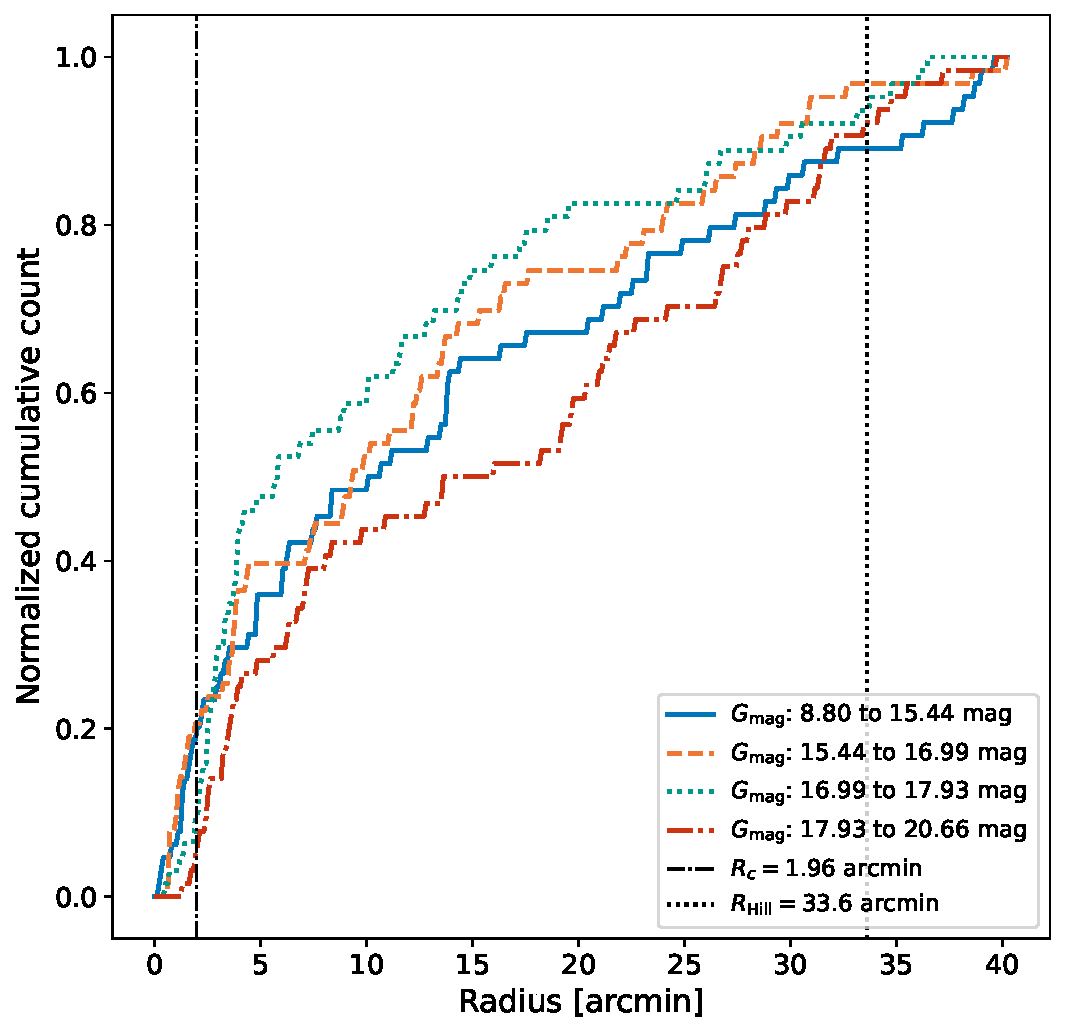
\includegraphics{Figures/cumulative_by_brightness_paper.pdf}}
	\caption{Normalized cumulative counts of reference-sample stars ($\tilde{p}\geq0.6$) within NGC 6383 are plotted against radial distance from the cluster center for different brightness ranges, segmented into quartiles of $G_{\text{mag}}$, whose ranges are given in the legend. The black dash-dotted and black dotted vertical lines mark the core radius $R_c = 1.96\,\mathrm{arcmin}$ and the Hill radius $R_{\mathrm{Hill}} = 33.6\,\mathrm{arcmin}$; the adopted King outer radius, $R_t = 54^{+7}_{-11}\,\mathrm{arcmin}$ (Appendix~\ref{app:window}), lies beyond the plotted range of this $40\,\mathrm{arcmin}$ sample.}
	\label{fig:cumulative_luminosity}
\end{figure}

The radial cumulative distributions of cluster members at various magnitude levels, illustrated in Fig. \ref{fig:cumulative_luminosity}, show that fainter stars, ranging from $17.93$ to $20.66\,\mathrm{mag}$, are less concentrated around the cluster's center. This observation is consistent with \textit{Gaia}'s completeness limit for magnitudes between $18$ and $19$ at distances around $1\,\mathrm{kpc}$ \citep{2020MNRAS.497.4246B,2023AA...677A..37C}. To test whether this reflects a real spatial difference, we compared the radial distribution of the faintest quartile with that of each of the three brighter quartiles using two-sample Kolmogorov-Smirnov (KS) tests. The faintest quartile differs from the two intermediate quartiles ($G=16.99$--$17.93\,\mathrm{mag}$: $D=0.28$, $p=0.010$; $G=15.44$--$16.99\,\mathrm{mag}$: $D=0.23$, $p=0.052$), but is statistically indistinguishable from the brightest quartile ($G=8.80$--$15.44\,\mathrm{mag}$: $D=0.16$, $p=0.42$); after a Holm correction for the three tests, only the difference with respect to the $16.99$--$17.93\,\mathrm{mag}$ quartile remains significant. If the lower central concentration of the faintest stars were caused by dynamical mass segregation, the contrast should be strongest with respect to the brightest (most massive) quartile, which is the opposite of what we find. We therefore attribute the apparent deficit of faint stars toward the crowded cluster center to \textit{Gaia} incompleteness at $G\gtrsim18\,\mathrm{mag}$ rather than to a dynamical effect.

We estimated individual stellar masses and binary probabilities with ASteCA v0.6.9 (Fig. \ref{fig:cmd_mass_binary}). These values, particularly for PMS stars, should be interpreted with caution because the PMS CMD is poorly defined \citep{2010ApJ...723..166D}, which limits isochrone-based mass and binarity estimates. Binary probabilities of at least $0.6$ define the binary class used throughout, consistent with the membership thresholds, while secondary masses are added to the system mass only for binary probability $>0.7$, a stricter cut that avoids inflating system masses through uncertain binary identifications.

Both the primary mass $m_1$ and the secondary mass $m_2$ are individual per-star estimates returned by ASteCA, not the product of an assumed universal mass ratio. For each of the $200$ synthetic-cluster realizations drawn from the posterior of the fitted parameters, every observed star is matched to its photometrically nearest synthetic star, whose primary and (when the match is a binary) secondary masses are recorded; $m_1$ and $m_2$ are the medians of these values over the realizations, and the binary probability is the fraction of realizations in which the match is a binary. The mass ratios of the synthetic binaries follow the \citet{2013ARA&A..51..269D} distribution introduced in Sect.~\ref{subsec:asteca}; for the $51$ stars whose secondary mass is added to the system mass (binary probability $>0.7$), the resulting mass ratios span $q=m_2/m_1=0.26$--$0.73$ with a median of $0.60$. The average mass of the stars is $1.31 \pm 0.10\,M_\odot$ (standard error on the mean, combining the sampling and per-star mass uncertainties), computed as the total mass per system (summing both components for binary probability $>0.7$) over the 254-member reference sample.

To investigate mass segregation, we constructed radial normalized cumulative mass distributions for single stars, binary stars, and the combination of both, as shown in Fig. \ref{fig:mass_seg}. A two-sample KS test comparing binary and single stars yields $D=0.221$ and $p=0.010$, indicating that binary stars are significantly more centrally concentrated. The signal is stable against the classification threshold ($D=0.21$--$0.29$, $p\leq0.018$ for binary-probability cuts of $0.5$--$0.8$) and is not solely a mass effect: restricting both classes to their overlapping mass range ($0.37$--$2.77\,M_\odot$) gives $D=0.19$, $p=0.07$, and a nearest-mass-matched comparison gives $D=0.36$, $p<0.001$, although mass and binarity remain partially entangled. Across single-star mass quartiles the KS results vary ($D=0.12$--$0.33$, $p=0.03$--$0.86$); given the width of these bins and the spread in $p$-values, we do not rely on any single quartile, and instead confirm the segregation with the bin-free $\Lambda_{\mathrm{MSR}}$ analysis (Fig. \ref{fig:mst}) below.

\begin{figure*}
	\centering
	\resizebox{\hsize}{!}{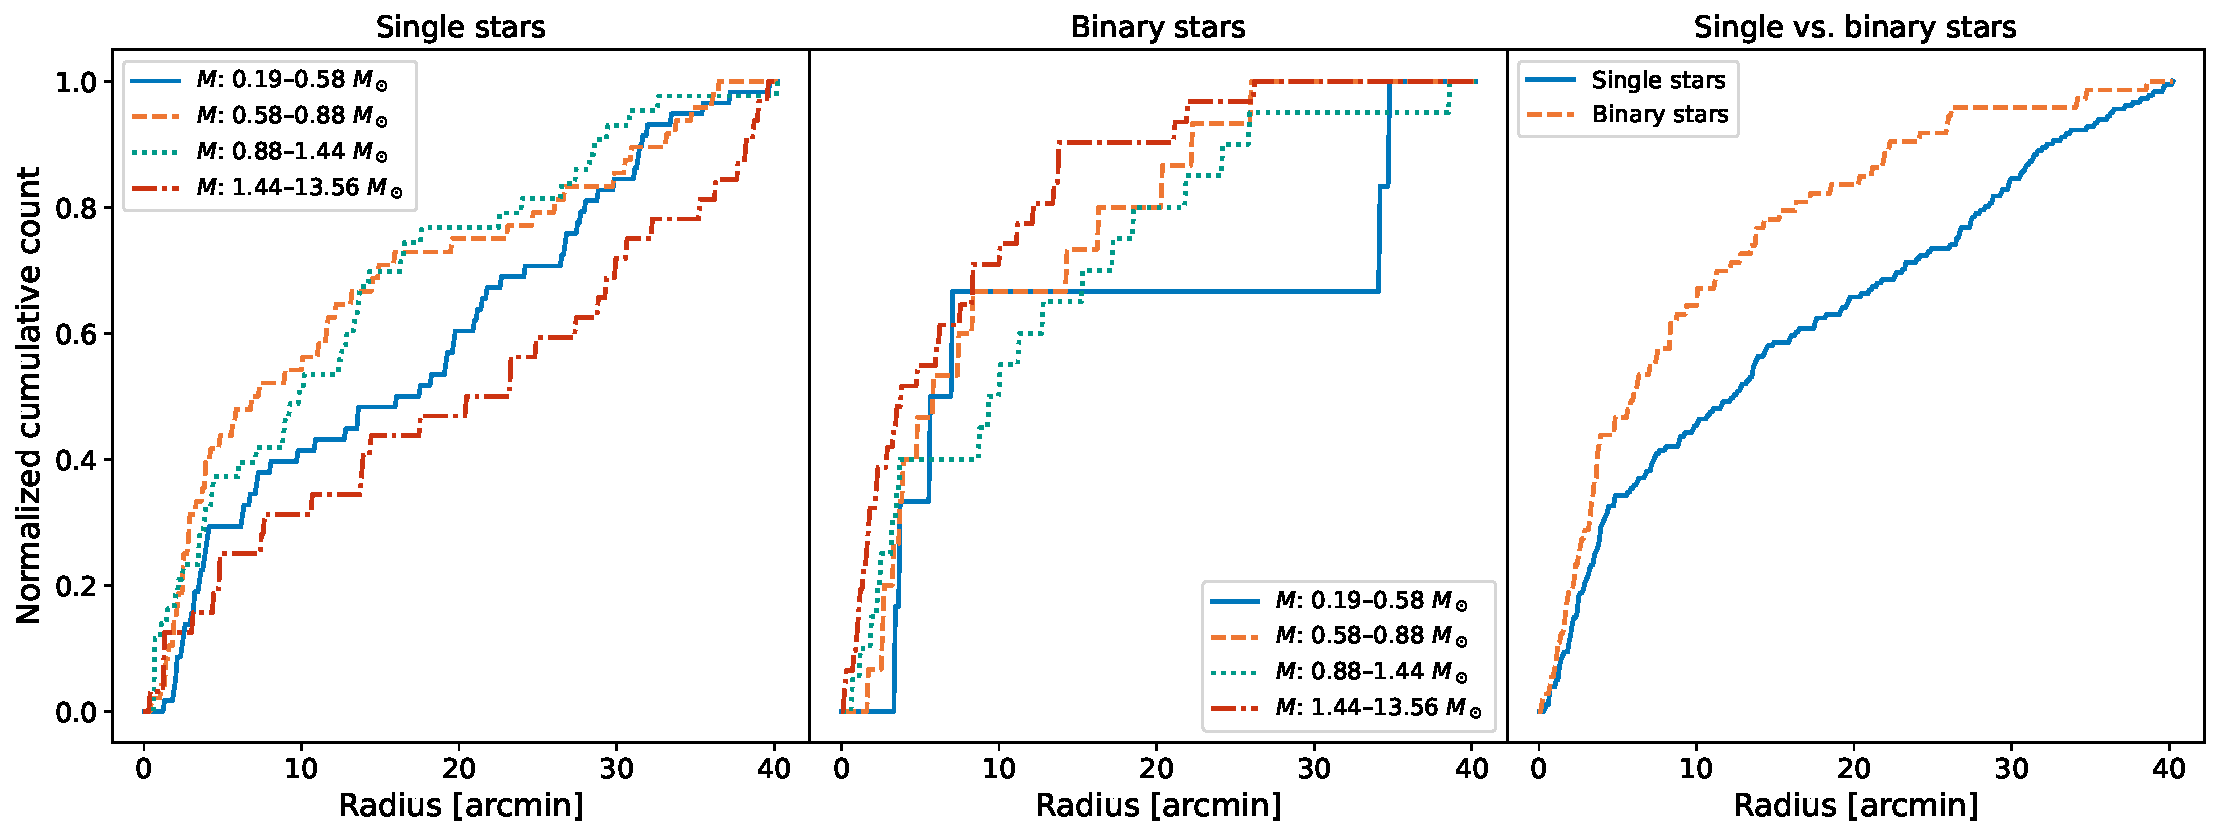
\includegraphics{Figures/cumulative_by_mass_and_type.pdf}}
    \caption{\emph{Left panel:} The cumulative distributions of single stars within NGC 6383 are segmented into four mass quartiles ranging from $0.19$--$0.58\,M_\odot$ to $1.44$--$13.56\,M_\odot$, illustrating the spatial distribution across different mass ranges and highlighting the potential influences of mass on the distribution of stars within the cluster. \emph{Middle panel:} The same distributions as in the left panel for binary stars only, where binaries are defined as sources with a binary probability of at least $0.6$. \emph{Right panel:} The normalized cumulative distributions compare single stars with binary stars, with masses between $0.19\,M_\odot$ and $13.56\,M_\odot$. All plots are based on stars with a membership pseudo-probability of at least $0.6$. The corresponding Kolmogorov-Smirnov (KS) test results are given in Sect. \ref{subsec:lum_mass_dyn}.}
	\label{fig:mass_seg}
\end{figure*}

To contextualize these findings, we calculated the half-mass relaxation time $t_{\mathrm{rh}}$ \citep{1969ApJ...158L.139S}, which is crucial for estimating the minimum mass segregation time $t_{\mathrm{seg}}$. The half-mass relaxation time is given by:

\begin{equation}
t_{\mathrm{rh}} = \frac{0.138\,N}{\ln(\gamma N)}\sqrt{\frac{r_{hm}^3}{GM}}
\end{equation}

where $N=254$ is the size of the reference sample, $\gamma = 0.110$ is the equal-mass Coulomb-logarithm constant \citep[not to be confused with the \textsc{HDBSCAN} density level $\lambda$ of Sect.~\ref{subsubsec:membership};][]{1994MNRAS.268..257G}, and $r_\mathrm{hm} = 2.02 \pm 0.41\,\mathrm{pc}$ is the half-mass radius, derived from the radial cumulative mass distribution. For self-consistency between $N$ and $M$, we take $M$ as the total observed mass of the same stellar system, $M = N\langle m \rangle = 332 \pm 26\,M_\odot$, rather than an IMF-extrapolated total cluster mass. The calculated half-mass relaxation time for NGC 6383 is $24.7\pm 7.6\,\mathrm{Myr}$ \citep{1971ApJ...164..399S}. For a system with a mass spectrum the effective Coulomb constant is smaller \citep[$\gamma\simeq0.02$;][]{1996MNRAS.279.1037G}, which would roughly double $t_{\mathrm{rh}}$; since all our dynamical-youth arguments rely on the cluster age being much shorter than $t_{\mathrm{rh}}$, adopting the equal-mass value is the conservative choice. The dependence of $\gamma$ on the mass spectrum is in fact available in closed form, as a functional of the mass function alone \citep[his Eqs.~11 and 26]{1975IAUS...69..133H}. Evaluating it on the observed mass distribution of the reference sample itself, holding $N$ and $M$ at the values above so that only $\gamma$ changes, gives $\gamma\simeq0.05$, between the equal-mass and the multi-mass values quoted above, and a $t_{\mathrm{rh}}$ larger by a factor $1.27$--$1.35$ (the range spanned by a kernel estimate of the mass function and by the discrete set of member masses), i.e. $t_{\mathrm{rh}}\simeq31$--$33\,\mathrm{Myr}$. We retain $\gamma=0.110$ throughout and carry this factor as a stated systematic: for the observed mass spectrum it lengthens $t_{\mathrm{rh}}$, and with it $t_{\mathrm{seg}}$ and $m_{\mathrm{lim}}$, so the values quoted below are conservative with respect to it.

Using the half-mass relaxation time, the timescale on which two-body relaxation drives a star of mass $m$ toward the cluster center can be estimated following \citet{1969ApJ...158L.139S}:

\begin{equation}\label{eq:tseg}
t_{\mathrm{seg}}(m) = \frac{\langle m \rangle}{m}\, t_{\mathrm{rh}},
\end{equation}

where $\langle m \rangle$ is the average stellar mass in the cluster: the more massive the star, the faster it segregates. For the most massive star of the reference sample ($13.56 \pm 3.25\,M_\odot$) this yields the minimum segregation time of the cluster, $t_{\mathrm{seg}} = 2.38 \pm 1.24\,\mathrm{Myr}$ (propagating the uncertainties in $\langle m \rangle$, $m$, and $t_{\mathrm{rh}}$); since this is shorter than the adopted cluster age, the most massive star has had time to segregate dynamically. The comparison is a marginal one rather than a strict inequality: the $1\sigma$ range of $t_{\mathrm{seg}}$ alone, $1.14$--$3.62\,\mathrm{Myr}$, already reaches the adopted age, and the lower edge of the age range of Sect.~\ref{subsec:asteca} ($2.24\,\mathrm{Myr}$) falls slightly below the central $t_{\mathrm{seg}}$. The mass-function value of $\gamma$ discussed above moves $t_{\mathrm{seg}}$ the same way, to $3.0$--$3.2\,\mathrm{Myr}$, and the multi-mass $\gamma\simeq0.02$ takes it to $\simeq4.9\,\mathrm{Myr}$, above the mode age; the sign of this comparison, for the single most massive member, is therefore not robust against the choice of Coulomb constant. It does not affect the argument that follows, which rests on the stars whose $t_{\mathrm{seg}}$ exceeds the cluster age: a longer $t_{\mathrm{rh}}$ adds members to that set rather than removing them. This value directly depends on the mass of the most massive member and would decrease if HD 159176, which we do not retain as a member (Sect.~\ref{subsubsec:hd159176}), belonged to the cluster. Adopting the component masses of $\simeq44$--$46\,M_\odot$ derived by \citet{2016ApJ...832..211P}, $t_{\mathrm{seg}}$ of the most massive object would drop to $\simeq0.7\,\mathrm{Myr}$ ($\simeq0.4\,\mathrm{Myr}$ if the binary is treated as a single $\sim90\,M_\odot$ body). This is a factor of $3$--$7$ shorter and would only reinforce this conclusion.

For all other stars, Eq.~(\ref{eq:tseg}) implies progressively longer segregation times. Setting $t_{\mathrm{seg}}(m)$ equal to the cluster age defines a limiting mass $m_{\mathrm{lim}} = \langle m \rangle\, t_{\mathrm{rh}}/t_{\mathrm{age}}$, which for the mode age $t_{\mathrm{age}} = 3.53\,\mathrm{Myr}$ and $\gamma=0.110$ is $9.1\,M_\odot$ (computed with unrounded posterior values); this is the value that defines the subsample used below. It is not a precise quantity. Across the age range of Sect.~\ref{subsec:asteca} it runs from $14.5\,M_\odot$ at the young edge to $3.6\,M_\odot$ at the old one, and the mass-function $\gamma$ raises it by the factor given above at every age, to $11.6$--$12.4\,M_\odot$ at the mode age. The argument is insensitive to this. Over that whole range the fraction of the reference sample below $m_{\mathrm{lim}}$ stays between $95\%$ and $100\%$; the subsample itself is identical for any $m_{\mathrm{lim}}$ between $8.49$ and $13.13\,M_\odot$, a window that contains both the adopted value and its $\gamma$-corrected counterpart; and at the young edge $m_{\mathrm{lim}}$ exceeds the mass of the most massive member, so at that edge no member of the sample has $t_{\mathrm{seg}}$ shorter than the cluster age. Stars less massive than the adopted $m_{\mathrm{lim}}$ have $t_{\mathrm{seg}}$ longer than the cluster age, so two-body relaxation cannot yet have segregated them: any central concentration they exhibit must be primordial or early dynamical. If HD 159176 were included as a member, $m_{\mathrm{lim}}$ would shift only to $\simeq10.3\,M_\odot$, leaving this subsample unchanged. We therefore repeated the analysis of Fig.~\ref{fig:mass_seg} for the subsample with $m < m_{\mathrm{lim}}$. This subsample comprises $252$ of the $254$ reference stars ($99.2\%$) and spans $0.19$--$8.49\,M_\odot$; only the two most massive members, of $13.13$ and $13.56\,M_\odot$, are excluded. The results (Fig.~\ref{fig:mass_tseg}) closely resemble Fig.~\ref{fig:mass_seg}, as expected for a nearly identical sample. Within this subsample the single-star quartile KS results range over $D=0.12$--$0.36$ and $p=0.01$--$0.84$, with the upper mass quartile ($1.41$--$8.49\,M_\odot$) showing the largest separation. In this sample, the average mass is $1.21 \pm 0.08\,M_\odot$. The distributions of single and binary stars are similar up to approximately $5\,\mathrm{arcmin}$, beyond which single stars show less concentration compared to binary stars.

As an independent, bin-free check of mass segregation, we computed the mass-segregation ratio $\Lambda_{\mathrm{MSR}}$ of \citet{2009MNRAS.395.1449A}, which compares the minimum-spanning-tree (MST) length of the $N_{\mathrm{MST}}$ most massive members with that of random sets of the same size. This estimator needs no cluster center, and for smooth, centrally concentrated regions it agrees with the other standard mass-segregation diagnostics \citep{2015MNRAS.449.3381P}. We verified that NGC 6383 belongs to this regime rather than being spatially substructured by computing the structure parameter $\mathcal{Q}$ of \citet{2004MNRAS.348..589C} (the ratio of the normalized mean MST edge length to the normalized mean projected separation, not to be confused with the reddening-free index $Q$ used above to identify YSOs). We obtain $\mathcal{Q}=1.03\pm0.03$ (bootstrap over the 254 members), well above the $\mathcal{Q}\simeq0.8$ boundary separating centrally concentrated from fractal, substructured distributions, and consistent with the King concentration $C=1.43$; we note that a proper-motion-selected, parallax-clipped sample is itself biased toward smooth configurations, so $\mathcal{Q}$ serves here as a consistency check rather than an independent morphology measurement. As shown in Fig. \ref{fig:mst}, $\Lambda_{\mathrm{MSR}}$ reaches $\approx2.5$--$3.6$ for the $5$--$15$ most massive members and decreases toward unity for larger samples, indicating that the most massive members are more centrally concentrated than typical members. We assessed the significance of this signal against an exact permutation null constructed on the observed member positions themselves, rather than against a null of exactly unity. Under the hypothesis that stellar mass is independent of position, the $N_{\mathrm{MST}}$ most massive stars occupy a uniform random $N_{\mathrm{MST}}$-subset of the observed positions, which is precisely what the $500$ reference sets already sample; the null distribution of $\Lambda_{\mathrm{MSR}}$ therefore follows from the same draws at no additional cost, and requires no assumption about the underlying radial profile. At the geometry of our reference sample the null median is $1.02$ at $N_{\mathrm{MST}}=5$ rather than exactly $1$, falling to unity for larger subsets, so the excess is measured from a slightly displaced origin. The strongest single point reaches a local $p\simeq5\times10^{-4}$; correcting for the eight values of $N_{\mathrm{MST}}$ examined, whose nesting yields a measured trials factor of about $7$ rather than the naive $8$, the scan-level significance is $p\approx0.004$, i.e. $\approx2.7\sigma$. This scan-level significance is unchanged if the members are ranked by primary mass instead of by system mass, which is the ranking cross-check required by the binary interpretation above, although the strongest individual point then falls at a different $N_{\mathrm{MST}}$: the per-point significance is sensitive to the mass ranking, and the scan-level result is not. The signal is unchanged in direction if the median edge length \citep{2011MNRAS.416..541M} or the geometric mean of the edge lengths \citep{2011A&A...532A.119O} replaces the total MST length, both of which limit the influence of a single long edge; the absolute values of the three variants are not directly comparable \citep{2011MNRAS.416..541M}, so only their sign and relative behavior are compared here. This bin-independent result supports the mass-segregation signal seen in the cumulative distributions.

The cluster is dynamically young, with an age of only $\simeq0.14\,t_{\mathrm{rh}}$, far below the $\sim2$--$3.5\,t_{\mathrm{rh}}$ over which primordial mass segregation is erased in $N$-body models, including those with a realistic primordial binary population \citep{2020A&A...638A.155P}. The intermediate-mass binaries that are centrally concentrated have segregation times longer than the cluster age, so two-body relaxation is too slow to explain their distribution, suggesting instead that they formed closer to the center than single stars.

Two-body relaxation is not the only dynamical route, however: cool or substructured clusters can segregate rapidly through the transient dense core formed during an early collapse \citep{2009ApJ...700L..99A}, and subcluster merging accelerates segregation even in the low-membership regime of local open clusters such as NGC 6383 \citep{2009MNRAS.400..657M}. Such early dynamical segregation also erases substructure, leaving a smooth, concentrated remnant like the one observed here ($\mathcal{Q}=1.03$); it is therefore observationally degenerate with genuine birth segregation. We describe the central concentration as primordial or near-primordial, where near-primordial encompasses rapid early dynamical segregation during cluster assembly. Simulations show that this configuration can be inherited if the cluster assembled from clumps that were already mass-segregated, or segregated before merging \citep{2007ApJ...655L..45M}, and can be amplified by residual-gas expulsion, which preferentially removes peripheral low-mass stars \citep{2007MNRAS.380.1589B}. A comparable primordial or near-primordial segregation is seen in other young clusters of similar age \citep{2007AJ....134.1368C,2008AJ....135..173S}.

Population-level studies caution against a purely primordial reading for young open clusters: applying $\Lambda_{\mathrm{MSR}}$ and related indicators to $3881$ \textit{Gaia} DR3 clusters, \citet{2026AJ....171..236Z} finds the spatial segregation of $<10\,\mathrm{Myr}$ systems to be statistically consistent with random and attributes classical segregation to two-body relaxation only beyond $\sim100\,\mathrm{Myr}$, and $N$-body models compared with observed open clusters similarly find primordial segregation not to be a decisive ingredient \citep{2026arXiv260604509A}. Our single-cluster detection therefore does not by itself settle the primordial-versus-dynamical question; we report the segregation as measured and its origin as primordial or early dynamical.

\begin{figure}
	\centering
	\resizebox{\hsize}{!}{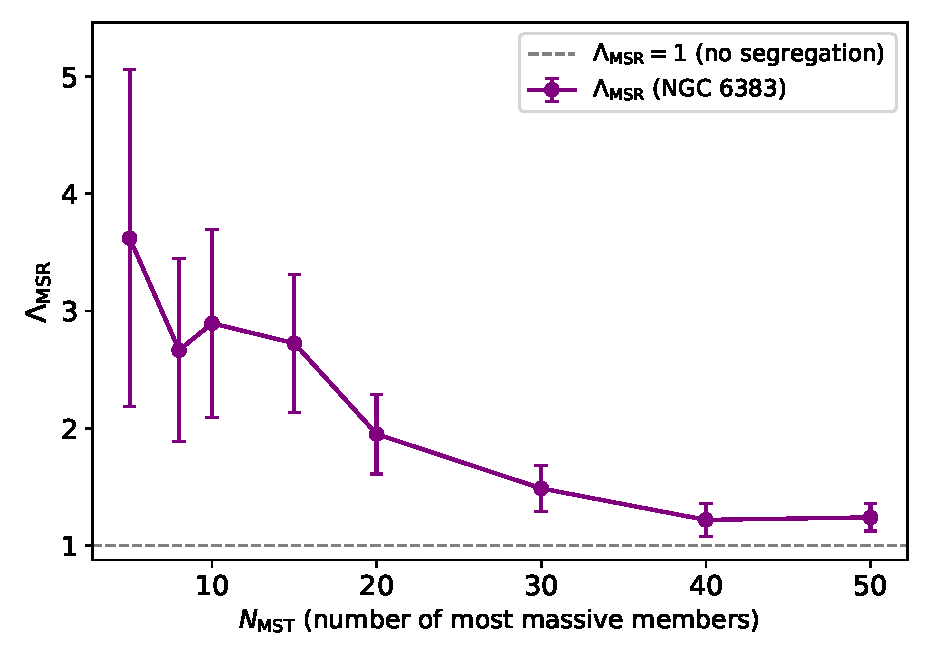
\includegraphics{Figures/mass_segregation_mst.pdf}}
	\caption{Mass-segregation ratio $\Lambda_{\mathrm{MSR}}$ \citep{2009MNRAS.395.1449A} of NGC 6383 as a function of the number of most-massive members $N_{\mathrm{MST}}$. Following \citet{2009MNRAS.395.1449A}, $\Lambda_{\mathrm{MSR}}=\langle l_{\mathrm{norm}}\rangle/l_{\mathrm{massive}}$ is the ratio of the mean minimum-spanning-tree length of $500$ random $N_{\mathrm{MST}}$-star sets to that of the $N_{\mathrm{MST}}$ most massive members (purple circles connected by a solid line); error bars are $\sigma_{\mathrm{norm}}/l_{\mathrm{massive}}$, following the convention of \citet{2009MNRAS.395.1449A}. They describe the spread of the random reference sets and are not the quantity from which the significance quoted in Sect.~\ref{subsec:lum_mass_dyn} is derived; that significance comes from the exact permutation null on the observed member positions. Values $\Lambda_{\mathrm{MSR}}>1$ indicate that the most massive stars are more centrally concentrated than random members; the gray dashed line marks $\Lambda_{\mathrm{MSR}}=1$ (no segregation).}
	\label{fig:mst}
\end{figure}

\section{Comparison with previous studies}\label{sec:comparison}
\subsection{HD 159176}\label{subsubsec:hd159176}
HD 159176 is a double-lined O-type spectroscopic binary projected close to the center of NGC 6383 and is responsible for ionizing the surrounding HII region \citep{1993Obs...113..204S,2007A&A...474..193L,2016ApJ...832..211P}. The estimated age of HD 159176 is $2.3$--$2.7\,\mathrm{Myr}$ \citep{2010AA...511A..25R}, in agreement with the earlier estimate of $2.8\pm0.5\,\mathrm{Myr}$ \citep{1978MNRAS.182..607F}. This estimate places the binary components, with the parameters of \citet{2007A&A...474..193L}, on single-star evolutionary tracks with and without rotation \citep{2003A&A...404..975M}, while the $2$--$3\,\mathrm{Myr}$ PMS ages of \citet{2010AA...511A..25R} rest on comparing X-ray-selected candidates with several PMS model families \citep[e.g.][]{2000A&A...358..593S}, and are therefore subject to the same code-dependent systematics discussed in Sect.~\ref{subsec:asteca}. The two age ranges are compatible, consistent with a common star-formation event if the binary is assumed to be associated with the cluster.

In the study by \citet{2018AA...610A..30A}, it was hypothesized that if HD 159176 were a blue straggler, it would imply an older age for NGC 6383, ranging between $6.00$ and $10.0\,\mathrm{Myr}$. We do not use this assumption in the present analysis. HD 159176 is classified in the spectroscopic literature as a double-lined O-type main-sequence binary, O7V((f))+O7V((f)) \citep{1993Obs...113..204S,2007A&A...474..193L} or O6.5V+O7V \citep{2016ApJ...832..211P}, and its thermal X-ray emission is attributed to the winds of the two O stars and their wind--wind interaction \citep{2003AA...407..925R,2004A&A...416..221D}; no accretion-powered scenario has been proposed for this system.

The \textit{Gaia} DR3 values of HD 159176 are $\varpi = 1.167 \pm 0.071\,\mathrm{mas}$, $\mu_{\alpha*}=2.621 \pm 0.083$, and $\mu_{\delta}=-0.798 \pm 0.058\,\mathrm{mas\,yr^{-1}}$. These must be treated cautiously: at $G\simeq5.7$ (vs $G_{\min}=8.80$ and median $G\simeq17.0$ for the reference sample) the star lies in the bright-source regime prone to saturation and magnitude-dependent astrometric systematics \citep{2021A&A...649A...2L,2021A&A...649A...4L,2021A&A...649A.124C,2022A&A...657A.130M}. The $\mu_{\alpha*}$ agrees with the cluster mean and the parallax offset is not by itself conclusive; the strongest tension is in $\mu_{\delta}$, which differs from the cluster mean ($-1.713\,\mathrm{mas\,yr^{-1}}$, dispersion $0.138$) by $\Delta\mu_{\delta}\simeq0.91\,\mathrm{mas\,yr^{-1}}$, about $6\sigma$ once the star's own proper-motion uncertainty is added in quadrature to the member dispersion. We note that the preprocessing parallax window ($0.750$--$1.10\,\mathrm{mas}$) already excludes the DR3 parallax of HD 159176, so its absence from the candidate sample is partly by construction; given the astrometric-quality caveats above, we read the $\mu_{\delta}$ tension as supporting, rather than decisive, evidence against membership.

\textit{Gaia} DR3 astrometric-quality indicators reinforce this: HD 159176 has a normal $\mathrm{RUWE}=0.937$, 13 visibility periods, and no duplicated-source flag, but an excess-noise significance of 135.6 and an IPD multi-peak fraction of 39, far above the reference-sample medians of zero (84th percentiles 1.53 and 0). These are not used as a membership criterion but confirm that HD 159176 must be treated as a special bright-source astrometric case \citep{2022MNRAS.510.2597R}.

We therefore exclude HD 159176 from the member sample used to characterize NGC 6383, its noteworthy projected central position notwithstanding. The age quoted for NGC 6383 in this paper is derived from the selected low-mass and PMS population and does not rely on the evolutionary status of HD 159176.

\subsection{NGC 6383 22}
NGC 6383 22\footnote{Cataloged in SIMBAD as Gaia DR3 4054615634716139264.} is identified as a $\lambda$ Boo star. These stars are chemically peculiar A-type stars with abundance anomalies attributed to the accretion of metal-poor material. In a spectroscopic survey of metal-weak and emission-line stars in the Southern Hemisphere, \citet{2020MNRAS.499.2701M} found that $\lambda$ Boo stars, including NGC 6383 22, exhibit excesses at longer wavelengths, suggestive of circumstellar disks. This characteristic aligns with other stars in NGC 6383 and those studied in \citet{2019MNRAS.484.5102K}. However, NGC 6383 22 is not retained in our \textit{Gaia}-selected member sample because, despite matching the position and parallax of the cluster, its proper motion ($\mu_{\alpha*} = 1.790 \pm 0.030\,\mathrm{mas\,yr^{-1}}$, $\mu_{\delta} = -2.710 \pm 0.024\,\mathrm{mas\,yr^{-1}}$) is more than $3\sigma$ away from the mean of the posterior distribution of $\mu$. This result indicates that this star is likely passing near or through the cluster.

\subsection{PMS studies using \texorpdfstring{H$\alpha$}{H-alpha} photometry and VPHAS+}

\citet{2019MNRAS.484.5102K} examined 55 classical T-Tauri stars (CTTS) in the star-forming region Sh 2-012 and NGC 6383, utilizing VPHAS+ optical and H$\alpha$ photometry and \textit{Gaia} astrometry. They reported a mean age of $2.8 \pm 1.6\,\mathrm{Myr}$ for these stars (the quoted uncertainty is the error on the mean; the dispersion of the individual ages is $3.4\,\mathrm{Myr}$, with an interquartile range of $1.4$--$3.8\,\mathrm{Myr}$), with masses between $0.3$ and $0.9\,M_\odot$ and a median mass of $0.5\,M_\odot$. Their ages and masses were obtained by interpolating the observed $r$ versus $r-i$ CMD positions against PARSEC evolutionary models reddened by $E(B-V)=0.32$ \citep{2012MNRAS.427..127B}. \citet{2019MNRAS.484.5102K} notes that the same data yield mean ages of $2.9\pm1.7$ and $3.5\pm2.4\,\mathrm{Myr}$ with the \citet{2011A&A...533A.109T} and \citet{2000A&A...358..593S} models, following the pattern reported by \citet{2015ApJ...808...23H}, so part of any difference from our MIST-based age reflects the choice of evolutionary code (Sect.~\ref{subsec:asteca}). A second part reflects the adopted distance: \citet{2019MNRAS.484.5102K} adopts $1.34\,\mathrm{kpc}$, from \textit{Gaia} DR2 parallaxes, against our DR3-based $1.11\,\mathrm{kpc}$. The two agree within $1.6\sigma$, but the $0.41\,\mathrm{mag}$ difference in distance modulus places the same stars at a higher luminosity in his analysis and therefore biases the interpolated ages young relative to ours; the interpolated masses shift in the same direction. Notably, $94\%$ of CTTS with near-infrared cross-matches conform to the near-infrared T-Tauri locus, and all stars with mid-infrared photometry showed signs of accreting circumstellar disks; the CTTS are concentrated around NGC 6383 and toward the bright rims of Sh 2-012.

Out of the 55 CTTS kinematic members of Sh 2-012, only 15 are cataloged as members or potential members of the cluster in this study, with most having a PMS probability over $0.6$\footnote{The four exceptions have PMS probabilities of 16, 12, 55, and 45\%.}. The difference in member selection is mainly methodological: \citet{2019MNRAS.484.5102K} selected CTTS primarily from photometric H$\alpha$ equivalent widths and then refined membership with a double-peaked Gaussian fit to the \textit{Gaia} proper motions, whereas our selection rests on proper-motion clustering. Only one T-Tauri source\footnote{Cataloged as Gaia DR3 4054567805963940352.} is likely a binary ($0.94$ probability according to our analysis); this source belongs to both our $\tilde{p}\geq0.6$ reference sample and the \citet{2019MNRAS.484.5102K} CTTS list.

We also cross-matched our 321 likely candidates with the UBVRI H$\alpha$ photometric catalog of \citet{2010AA...511A..25R}. Using a $1.0\,\mathrm{arcsec}$ matching radius, we found 141 counterparts, including 124 sources from the $\tilde{p}\geq0.6$ reference sample. Their CDS table provides the $R_C-$H$\alpha$ index but not a published source-by-source H$\alpha$ emitter flag. We therefore do not treat the match as a recovery of the original Rauw et al. emitter list. Instead, we used their published $R_C-$H$\alpha$ color offsets ($0.12$--$0.24\,\mathrm{mag}$ above the main-sequence relation for candidates, $>0.24\,\mathrm{mag}$ for emitters) as a diagnostic relative to an empirical non-emitter locus derived from their catalog. Under this diagnostic classification, 51 of the 141 matched sources show H$\alpha$ excesses, including 28 of the 57 matched Sagitta PMS candidates. For the reference sample alone, 23 of the 51 matched Sagitta PMS candidates show such an excess. These matches support the presence of an emission-line subset among the PMS candidates, but the absence of diagnostic H$\alpha$ excess for the remaining PMS candidates is not decisive because \citet{2010AA...511A..25R} emphasized that H$\alpha$ emission is variable, can be weak for part of the PMS population, and that H$\alpha$-selected samples can be contaminated by foreground and background objects.

\subsection{Comparison with published catalogs}
We compared our likely-candidate catalog (see also the historical compilation in Appendix~\ref{app:historical}) with the catalogs from \citet{2020AA...640A...1C}, \citet{2021ApJ...923..129J}, \citet{2022ApJS..262....7H}, \citet{2024arXiv240305143H}, and the members listed in SIMBAD. We find 148 sources in common with \citet{2020AA...640A...1C}, 97 present only in their catalog, and 173 only in ours; 161 in common with \citet{2021ApJ...923..129J} (123 only theirs, 160 only ours); 90 with \citet{2022ApJS..262....7H} (47 only theirs, 231 only ours); 202 with \citet{2024arXiv240305143H} (120 only theirs, 119 only ours); and 168 with SIMBAD (163 only there, 153 only ours). Because all rely at least partly on \textit{Gaia} astrometry, the differences mainly reflect methodological choices, spatial windows, probability thresholds, and whether PMS or photometric information enters the selection. In particular, our selection clusters in the proper-motion plane only, whereas most catalog pipelines cluster in the full three- to five-dimensional astrometric space with their own probability floors and search radii, and SIMBAD aggregates heterogeneous literature memberships.

These overlaps also delimit the added value of the present analysis. These survey catalogs are homogeneous all-sky compilations optimized for thousands of clusters: for any individual cluster they provide a member list and bulk parameters derived from a single, fixed pipeline configuration. For NGC 6383, this work adds four elements. (i) Sampled posterior distributions, with reported uncertainties and convergence diagnostics, for the mean astrometric parameters, the parallax-based distance and the King structural parameters, rather than pipeline point estimates; for the isochrone fit we report the ensemble together with the explicit statement that it has not converged (Sect.~\ref{subsec:cosmic}), and adopt a systematic age range instead of a posterior width, which is itself information a fixed-pipeline catalog does not provide. (ii) An explicit sensitivity budget for the main configuration choices, which none of the above catalogs quantify on a per-cluster basis: the \textsc{HDBSCAN} hyperparameter sweep is marginalized into the per-star pseudo-probabilities (Sect.~\ref{subsubsec:membership}, Appendix~\ref{app:hdbscan}), the dependence of the membership and structural parameters on the search window is measured directly (Appendix~\ref{app:window}), and the mass-segregation signal is checked for stability against the binary-classification threshold (Sect.~\ref{subsec:lum_mass_dyn}). (iii) Cluster-specific analyses that survey pipelines do not attempt, namely the PMS census (Sagitta probabilities, ages, and extinctions; the YSO fraction; and the H$\alpha$ cross-match with \citealt{2010AA...511A..25R}), the dynamical-state analysis ($t_{\mathrm{rh}}$, $t_{\mathrm{seg}}$, $\Lambda_{\mathrm{MSR}}$), per-star masses and binary probabilities, and the individual treatment of HD 159176 as a bright-source astrometric special case. (iv) A per-star catalog at the CDS (Table~\ref{tab:cds_members}) together with the open-source pipeline, which make the selection reproducible and its parameter dependence auditable.

Where a derived quantity does depend on a configuration choice (most notably the outer membership and the King outer radius with respect to the search window) we flag it explicitly as window- or model-dependent rather than reporting it as a robust measurement (Sect.~\ref{subsec:structural}, Appendix~\ref{app:window}). The survey catalogs remain the appropriate reference for homogeneous population-level comparisons across clusters; we regard the two approaches as complementary rather than competing.

The adopted King outer radius also merits comparison with the literature. Published outer or tidal radii for NGC 6383 span $15$--$30\,\mathrm{arcmin}$ (Table~\ref{tab:literature}), all smaller than our $R_t=54^{+7}_{-11}\,\mathrm{arcmin}$, although the largest of them is consistent with it at the ${\sim}2\sigma$ level. The difference is expected in direction: those determinations were limited either by extractions comparable to or smaller than the radii they report or by the depth of the underlying survey data, so, like our own $40\,\mathrm{arcmin}$ fit ($R_t=40^{+16}_{-17}\,\mathrm{arcmin}$), their outer radii are limited by the available field, whereas our adopted value comes from the only extraction with a fitted background annulus beyond the cluster (Appendix~\ref{app:window}). The comparison therefore mostly reflects the window and background treatment, reinforcing our reading of $R_t$ as a model- and prior-dependent outer scale rather than a sharp physical boundary.

\section{Conclusions}\label{sec:conclusion}

This study presents an analysis of the young open cluster NGC 6383, employing Bayesian analysis and machine-learning techniques to identify cluster members and determine key parameters. Using the HDBSCAN algorithm in proper-motion space followed by parallax clipping, we identified 321 likely cluster candidates with $\tilde{p}>0.5$. The reference sample used for the cluster parameters contains 254 sources with membership pseudo-probabilities of at least 60\%.

Our findings indicate that the cluster has a mode age of $\simeq3.5~\mathrm{Myr}$ ($\log(\mathrm{age}\,\mathrm{yr^{-1}}) = 6.55^{+0.40}_{-0.20}$, the uncertainty being dominated by pre-main-sequence model systematics that act toward older ages), with a distance of $1.11 \pm 0.06\,\mathrm{kpc}$ derived from the parallax-based distance estimation. The core radius is $1.96^{+0.19}_{-0.16}\,\mathrm{arcmin}$; the King outer radius, measured on the $70\,\mathrm{arcmin}$ extraction that fully encloses the fitted profile, is $54^{+7}_{-11}\,\mathrm{arcmin}$, conditional on the prior bound that truncates its posterior from above (Sect.~\ref{subsec:structural}, Appendix~\ref{app:window}). Wider-field tests with $50$, $60$, and $70\,\mathrm{arcmin}$ input cones recover an NGC 6383-like proper-motion branch and a consistent outer radius in all cases, but the selected outer membership is not invariant with field size (Table \ref{tab:cone_params}, Appendix \ref{app:window}). In line with \textit{Gaia}-based work on open-cluster structure and tidal features \citep{2025MNRAS.539.2513A,2025A&A...694A.258R,2025A&A...698A.156X}, $R_t$ should therefore be regarded as a model-dependent scale rather than as an independently measured physical boundary.

The CMD analysis revealed a well-defined main sequence and a population of PMS stars, with an apparent age spread of $1.6$--$6.3\,\mathrm{Myr}$, consistent with a recent and possibly extended star-formation episode. The Sagitta neural network provided additional insights into the probabilities of PMS stars, their ages, and the extinction affecting cluster members. A cross-match with the UBVRI H$\alpha$ catalog of \citet{2010AA...511A..25R} identifies a diagnostic H$\alpha$-excess subset among the matched PMS candidates, consistent with an emission-line or accreting component.

HD 159176 is projected near the cluster center, but its \textit{Gaia} DR3 proper motion in declination is inconsistent with the selected cluster population; even allowing for the bright-source astrometric caveats discussed in Sect.~\ref{subsubsec:hd159176}, the tension is large enough that we exclude it from the member sample used for the cluster characterization. The age estimate reported here is derived from the selected PMS and low-mass population, as in previous PMS-based studies, and does not depend on assuming any particular evolutionary state for HD 159176.

The central concentration of binaries, even for those with segregation times longer than the cluster's age, suggests that they formed closer to the cluster center, pointing to a primordial or early dynamical origin for the segregation. As discussed in Sect.~\ref{subsec:lum_mass_dyn}, this reading is consistent with simulations of clump merging and gas expulsion and with the segregation observed in other young clusters, although population-level analyses find little statistically significant spatial segregation in clusters younger than $\sim10\,\mathrm{Myr}$ \citep{2026AJ....171..236Z}; our per-cluster result does not resolve this debate.

This work combines machine-learning membership with Bayesian parameter estimation to deliver an updated characterization of NGC 6383, and provides a template for similar studies of open-cluster candidates in the \textit{Gaia} era. The software used in this study is available on GitHub\footnote{\href{https://github.com/notluquis/erotica}{https://github.com/notluquis/erotica}}, and the catalog is available at the CDS (see Data availability).

\section*{Data availability}
The full 321-source likely-member catalog (Table~\ref{tab:cds_members}) is available in electronic form at the CDS via anonymous ftp to \texttt{cdsarc.cds.unistra.fr} (\texttt{130.79.128.5}) or via \url{https://cdsarc.cds.unistra.fr/viz-bin/cat/J/A+A/}. The \textsc{EROTICA} software used for this analysis is archived at \url{https://doi.org/10.5281/zenodo.21769959} and developed at \url{https://github.com/notluquis/erotica}.

\begin{acknowledgements}
This research has made use of the SIMBAD database and the VizieR catalogue access tool, operated at CDS, Strasbourg, France. We gratefully acknowledge support by the ANID BASAL project FB210003 and the SOCHIAS GEMINI project 32230014.

L.P. gratefully acknowledges the invaluable comments and guidance of Dr. Robert Mathieu in the preparation of this investigation, and financial support from the Dirección de Postgrado, Universidad de Concepción, through the MSc scholarship program. P.C. thanks the support of the UdeC VRID Iniciación fund 2025001386INI.

This work has made use of data from the European Space Agency (ESA) mission \textit{Gaia} (\url{https://www.cosmos.esa.int/gaia}), processed by the \textit{Gaia} Data Processing and Analysis Consortium (DPAC, \url{https://www.cosmos.esa.int/web/gaia/dpac/consortium}). Funding for the DPAC has been provided by national institutions, in particular the institutions participating in the \textit{Gaia} Multilateral Agreement. 

This publication makes use of data products from the Two Micron All Sky Survey, which is a joint project of the University of Massachusetts and the Infrared Processing and Analysis Center/California Institute of Technology, funded by the National Aeronautics and Space Administration and the National Science Foundation. The DSS2-red background image used in Fig. \ref{fig:real_sky} is based on the Digitized Sky Survey, produced at the Space Telescope Science Institute under U.S. Government grant NAG W-2166. This work made use of Astropy:\footnote{\url{http://www.astropy.org}} a community-developed core Python package and an ecosystem of tools and resources for astronomy \citep{astropy:2013, astropy:2018, astropy:2022}.
\end{acknowledgements}

\bibliographystyle{aa}
\bibliography{cites} 

\begin{appendix}
\nolinenumbers  % aa.cls re-enables line numbers inside \appendix; the body has them off

\section{Historical parameters of NGC 6383}\label{app:historical}

Table \ref{tab:literature} compiles the structural and fundamental parameters of NGC 6383 reported in the literature since \citet{1930LicOB..14..154T}. The wide spread of historical core and tidal radii, distances, reddenings, distance moduli, and ages, obtained with heterogeneous data and methods over nearly a century, illustrates the lack of a homogeneous determination and motivates the \textit{Gaia}-based reanalysis presented in this work. For each study we list only the quantities explicitly reported; ellipses denote parameters not provided.

\begin{table*}
\caption{Historical review of observed parameters for the open cluster NGC 6383. The table details the number of cluster members, core and tidal radii, parallax, distance, E(B-V) color excess, distance modulus $(m - M)$, and estimated ages. The literature tidal radii are King tidal radii, here denoted the King outer radius $R_t$, except \citet{2005AA...438.1163K}, whose value is their empirical cluster (corona) radius; the \citet{2008AA...477..165P} value is their $r_t$ ($8.3\pm1.2$ pc at their adopted distance). The ages are not derived on a common distance scale: the adopted distances in this table span $0.83$--$1.70\,\mathrm{kpc}$, a range of $1.6\,\mathrm{mag}$ in distance modulus, and an age obtained by placing stars on evolutionary tracks moves systematically with that choice. The listed ages should therefore be compared with the corresponding distance, not in isolation.}
\label{tab:literature}
\centering
\resizebox{\hsize}{!}{%
\begin{tabular}{llllllllllll}
\hline\hline
Reference & Members & Core Radius & Tidal Radius & Parallax & Distance & E(B-V) & $(m - M)$ & Age\\
& & $\mathrm{arcmin}$ & $\mathrm{arcmin}$ & $\mathrm{mas}$ & $\mathrm{kpc}$ & $\mathrm{mag}$ & $\mathrm{mag}$ & $\mathrm{Myr}$\\
\hline
\citet{1930LicOB..14..154T} & $\cdots$ & $\cdots$ & $\cdots$ & $\cdots$ & 2.13 & $\cdots$ & $\cdots$ & $\cdots$\\
\citet{1949ApJ...110..117S} & $\cdots$ & $\cdots$ & $\cdots$ & $\cdots$ & 0.76 & $\cdots$ & $\cdots$ & $\cdots$\\
\citet{1961RGOB...27...61E} & $\cdots$ & $\cdots$ & $\cdots$ & $\cdots$ & $\cdots$ & 0.30 & $\cdots$ & $\cdots$\\
\citet{1967MNRAS.135..377G} & 74 & $\cdots$ & $\cdots$ & $\cdots$ & 1.38 & $\cdots$ & 10.7$\pm$0.5 & $\cdots$\\
\citet{1968PhDT........29E} & At least 21 & $\cdots$ & $\cdots$ & $\cdots$ & 1.30 & 0.35 & 10.6 & 5.0\\
\citet{1968ArA.....5....1L} & $\cdots$ & $\cdots$ & $\cdots$ & $\cdots$ & 1.25 & $\cdots$ & 10.5 & $\sim$ 20\\
\citet{1971AAS....4..241B} & $\cdots$ & $\cdots$ & $\cdots$ & $\cdots$ & 1.07 & 0.26 & 10.9 & $\cdots$\\
\citet{1978MNRAS.182..607F} & $\cdots$ & 1.25 & $\cdots$ & $\cdots$ & 1.50$\pm$0.20 & 0.33$\pm$0.02 & 10.9 & 1.7$\pm$0.4\\
\citet{1978MNRAS.184..661L} & $\cdots$ & $\cdots$ & $\cdots$ & $\cdots$ & 1.35 & 0.35 & 10.6 & Up to 5.0\\
\citet{1985AA...151..391T} & $\cdots$ & $\cdots$ & $\cdots$ & $\cdots$ & 1.40$\pm$0.15 & 0.30$\pm$0.01 & $\cdots$ & $\cdots$\\
\citet{1989MNRAS.236..263P} & $\cdots$ & $\cdots$ & $\cdots$ & $\cdots$ & $\cdots$ & 0.35 & 11.7 & $\sim$ 4.5\\
\citet{1991MNRAS.249...76B} & 27 & $\cdots$ & $\cdots$ & $\cdots$ & 1.38 & 0.34 & $\cdots$ & $\sim$ 20\\
\citet{1994RMxAA..29..141F} & $\cdots$ & $\cdots$ & $\cdots$ & $\cdots$ & 1.40 & 0.33 & $\cdots$ & $\cdots$\\
\citet{2003AA...407..925R} & $\cdots$ & $\cdots$ & $\cdots$ & $\cdots$ & $\cdots$ & 0.33 & 10.7 & $\cdots$\\
\citet{2005AA...438.1163K} & 13 & 4.80 & 15.0 & $\cdots$ & 0.99 & 0.30 & 10.9 & 5.0\\
\citet{2007AA...462..157P} & $\cdots$ & $\cdots$ & $\cdots$ & $\cdots$ & 1.70$\pm$0.30 & 0.29$\pm$0.05 & $\cdots$ & Less than 4.0\\
\citet{2008AA...477..165P} & $\cdots$ & $\cdots$ & 29.0$\pm$4.2 & $\cdots$ & 0.99 & 0.30 & 10.9 & 5.0\\
\citet{2010AA...511A..25R} & 55 PMS candidates & $\cdots$ & $\cdots$ & $\cdots$ & $\cdots$ & 0.32 & $\cdots$ & 2--3\\
\citet{2018AA...610A..30A} & $\cdots$ & $\cdots$ & $\cdots$ & $\cdots$ & 0.83$\pm$0.16 & 0.51$\pm$0.03 & 9.61$\pm$0.38 & $\sim$3--10\\
\citet{2019MNRAS.484.5102K} & At least 55 & $\cdots$ & $\cdots$ & $\cdots$ & 1.34$\pm$0.13 & 0.32 & $\cdots$ & 2.8$\pm$1.6\\
\citet{2021ApJ...923..129J} & 284 & $\cdots$ & $\cdots$ & 0.93$\pm$0.09 & 1.07 & $\cdots$ & $\cdots$ & $\cdots$\\
\citet{2022ApJS..262....7H} & $\cdots$ & $\cdots$ & $\cdots$ & 0.88$\pm$0.05 & $\cdots$ & 0.45 & $\cdots$ & 3.5\\
\citet{2024arXiv240305143H} & 322 & 2.49 & 22.7 & 0.89$\pm$0.08 & 1.10 & 0.38 & 10.2 & $\sim$ 4.0\\
\citet{2024arXiv240301030P} & 266 & 1.21$\pm$0.13 & 29.7$\pm$7.7 & 0.92$\pm$0.06 & 1.10$\pm$0.04 & 0.47$\pm$0.03 & 10.9$\pm$0.33 & $\sim$1--4\\
\hline
\end{tabular}}
\end{table*}

\section{HDBSCAN diagnostic and ASteCA isochrone-fit corner plots}\label{app:hdbscan}

This appendix documents the unsupervised-clustering diagnostics and the isochrone-fit ensemble that underpin the membership and parameter determinations of Sects.~\ref{sec:membership} and \ref{subsec:asteca}. We first describe how the HDBSCAN configuration was selected from the proper-motion clustering sweep (Figs. \ref{fig:min_cluster_size} and \ref{fig:condensed_cluster_tree}), show the resulting clustering of the full sample in the proper-motion plane and on the sky (Fig. \ref{fig:pm_overview}), and then present the joint distribution of the ASteCA isochrone fit (Fig. \ref{fig:plot_pair_trace}).

HDBSCAN was run over the grid $m_{\mathrm{cl}}=10,\ldots,299$ in the two-dimensional proper-motion plane, setting \texttt{min\_cluster\_size}=\texttt{min\_samples}=$m_{\mathrm{cl}}$ and using the \texttt{leaf} cluster-selection method (Sect. \ref{subsubsec:membership}). For each run we recorded the size of the recovered NGC 6383 branch (the condensed-tree branch containing the highest density level $\lambda_{\mathrm{max}}$; Sect.~\ref{subsubsec:membership}) and its $\lambda_{\mathrm{max}}$. Figure~\ref{fig:min_cluster_size} displays the runs in the stable regime, delimited by $\lambda_{\mathrm{max}}\geq8$ and a recovered branch of $200$--$701$ sources (the upper bound being the largest branch recovered in the sweep); below $\lambda_{\mathrm{max}}=8$ the condensed tree is too shallow to separate the cluster from the field. These display cuts do not enter the selection: as Fig.~\ref{fig:min_cluster_size} shows, the recovered branch size peaks at the adopted $m_{\mathrm{cl}}=43$, with smaller $m_{\mathrm{cl}}$ fragmenting the cluster into spurious sub-groups and larger $m_{\mathrm{cl}}$ progressively merging field stars into the branch or dissolving it altogether.

\begin{figure}
\centering
\resizebox{\hsize}{!}{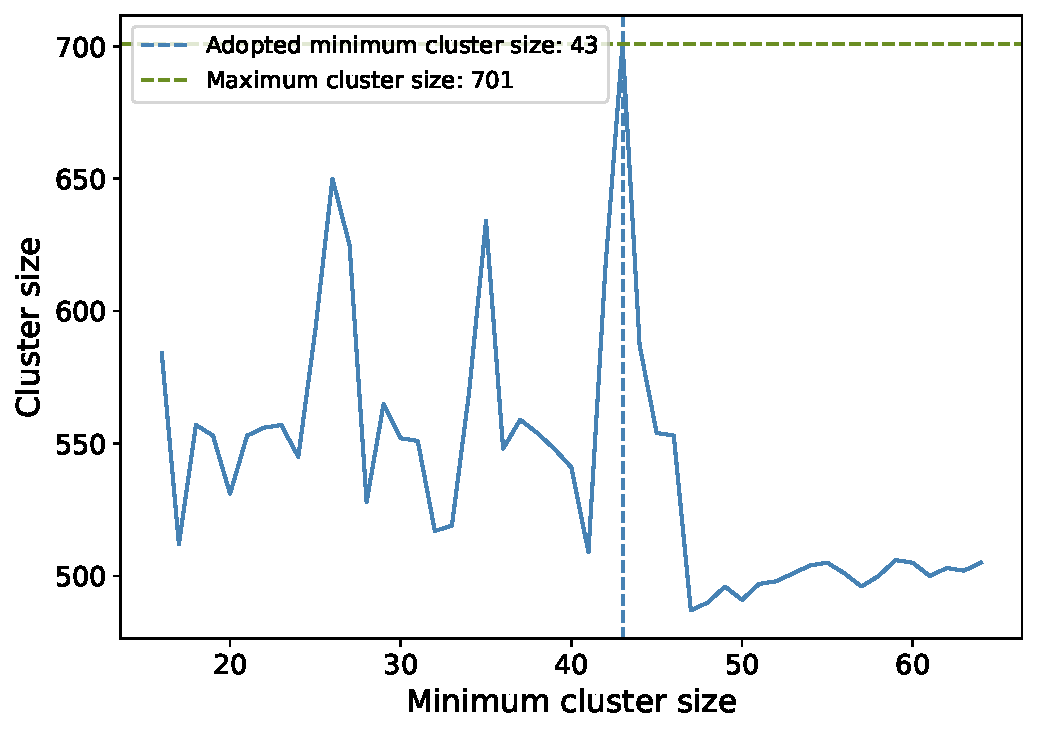
\includegraphics{Figures/min_cluster_size.pdf}}
\caption{Cluster size variation as a function of minimum cluster size, determined through HDBSCAN clustering on the proper-motion data of the sources. The blue line shows the recovered cluster size; the dashed blue line marks the adopted minimum cluster size of 43, where the cluster size peaks, and the dashed green line the maximum observed cluster size of 701. Only sweep runs in the stable regime ($\lambda_{\mathrm{max}}\geq8$ and recovered branch of $200$--$701$ sources) are shown, which is why the axis does not span the full $m_{\mathrm{cl}}=10$--$299$ grid; this display cut does not enter the selection of $m_{\mathrm{cl}}$.}
\label{fig:min_cluster_size}
\end{figure}

The condensed cluster tree (Fig. \ref{fig:condensed_cluster_tree}) displays the HDBSCAN hierarchy as a function of the density level $\lambda=1/d_{\mathrm{mreach}}$, where wider and more persistent branches correspond to denser, more significant over-densities. The NGC 6383 branch (the tall blue ellipse on the left) persists over the widest $\lambda$ interval and is clearly detached from the field branches on the right, providing the qualitative counterpart of the quantitative stability criterion used in Fig. \ref{fig:min_cluster_size}. This persistence is what allows the proper-motion over-density of NGC 6383 to be selected unambiguously, despite the known tendency of HDBSCAN to report spurious dense fluctuations in noisy data \citep{2021A&A...646A.104H}.

\begin{figure}
\resizebox{\hsize}{!}{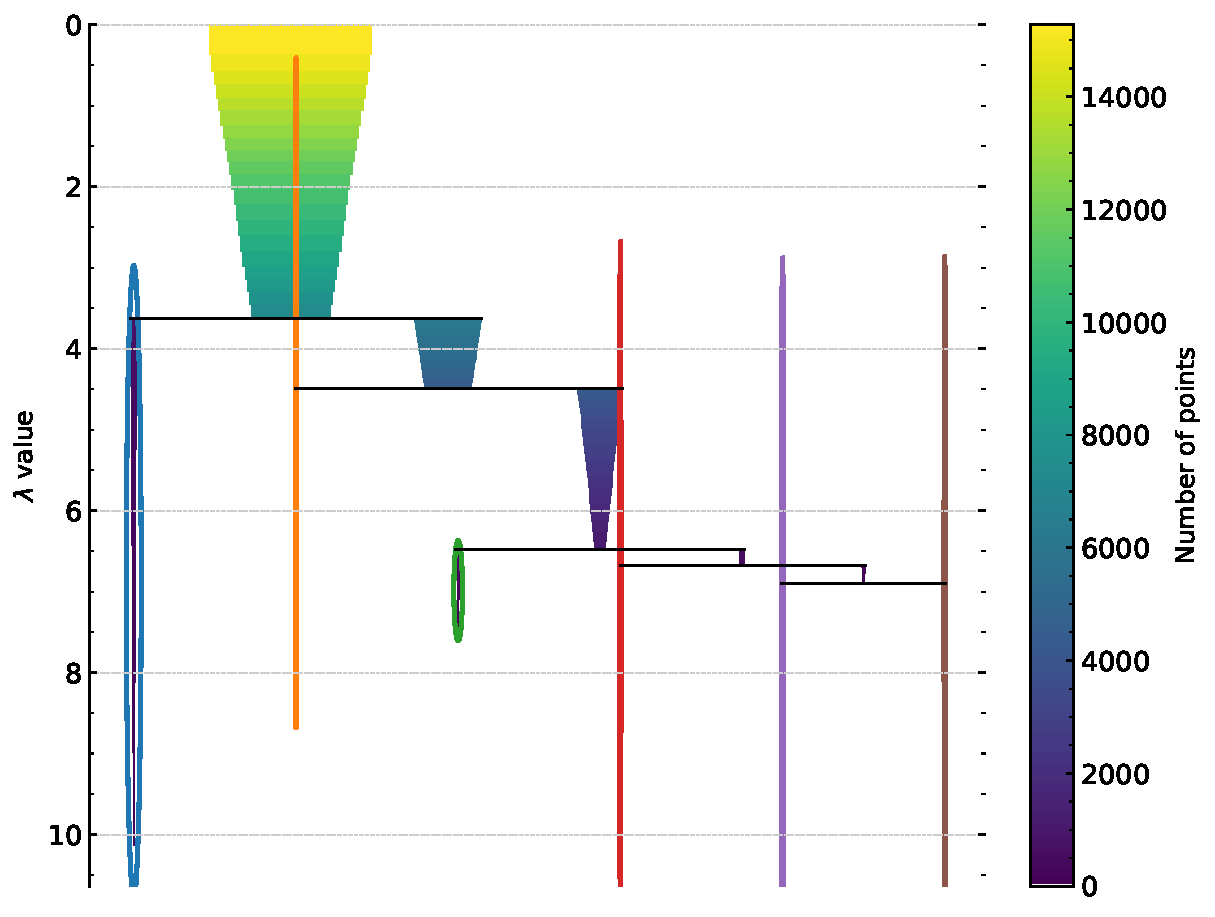
\includegraphics{Figures/condensed_cluster_tree_NGC6383.pdf}}
\caption{Condensed cluster tree (dendrogram) from the HDBSCAN analysis: NGC 6383 cluster sources on the left, HDBSCAN-identified field sources on the right. Branch width and color give the number of sources at each level (color bar); $\lambda=1/d_{\mathrm{mreach}}$ is the inverse mutual-reachability distance. Colored ellipses mark the leaf clusters selected by HDBSCAN; the tall blue ellipse on the left, persisting over the widest $\lambda$ range, is the branch adopted as NGC 6383.}
\label{fig:condensed_cluster_tree}
\end{figure}

Figure \ref{fig:pm_overview} places the selected branch in context, showing the full $40\,\mathrm{arcmin}$ preprocessed sample ($15276$ sources) labeled by HDBSCAN, both in the proper-motion plane and on the sky. In proper motion, NGC 6383 forms a compact, well-isolated over-density around $(\mu_{\alpha}^{*},\mu_{\delta})=(2.5,-1.7)\,\mathrm{mas\,yr^{-1}}$, clearly separated from the diffuse field and from the other, more dispersed HDBSCAN branches. On the sky, by contrast, the three groups overlap, with only a mild central concentration of the cluster members. This confirms that the membership signal is carried by the proper motions rather than by projected position, justifying the proper-motion-only clustering feature space adopted in Sect. \ref{subsubsec:membership}.

\begin{figure*}
\centering
\resizebox{\hsize}{!}{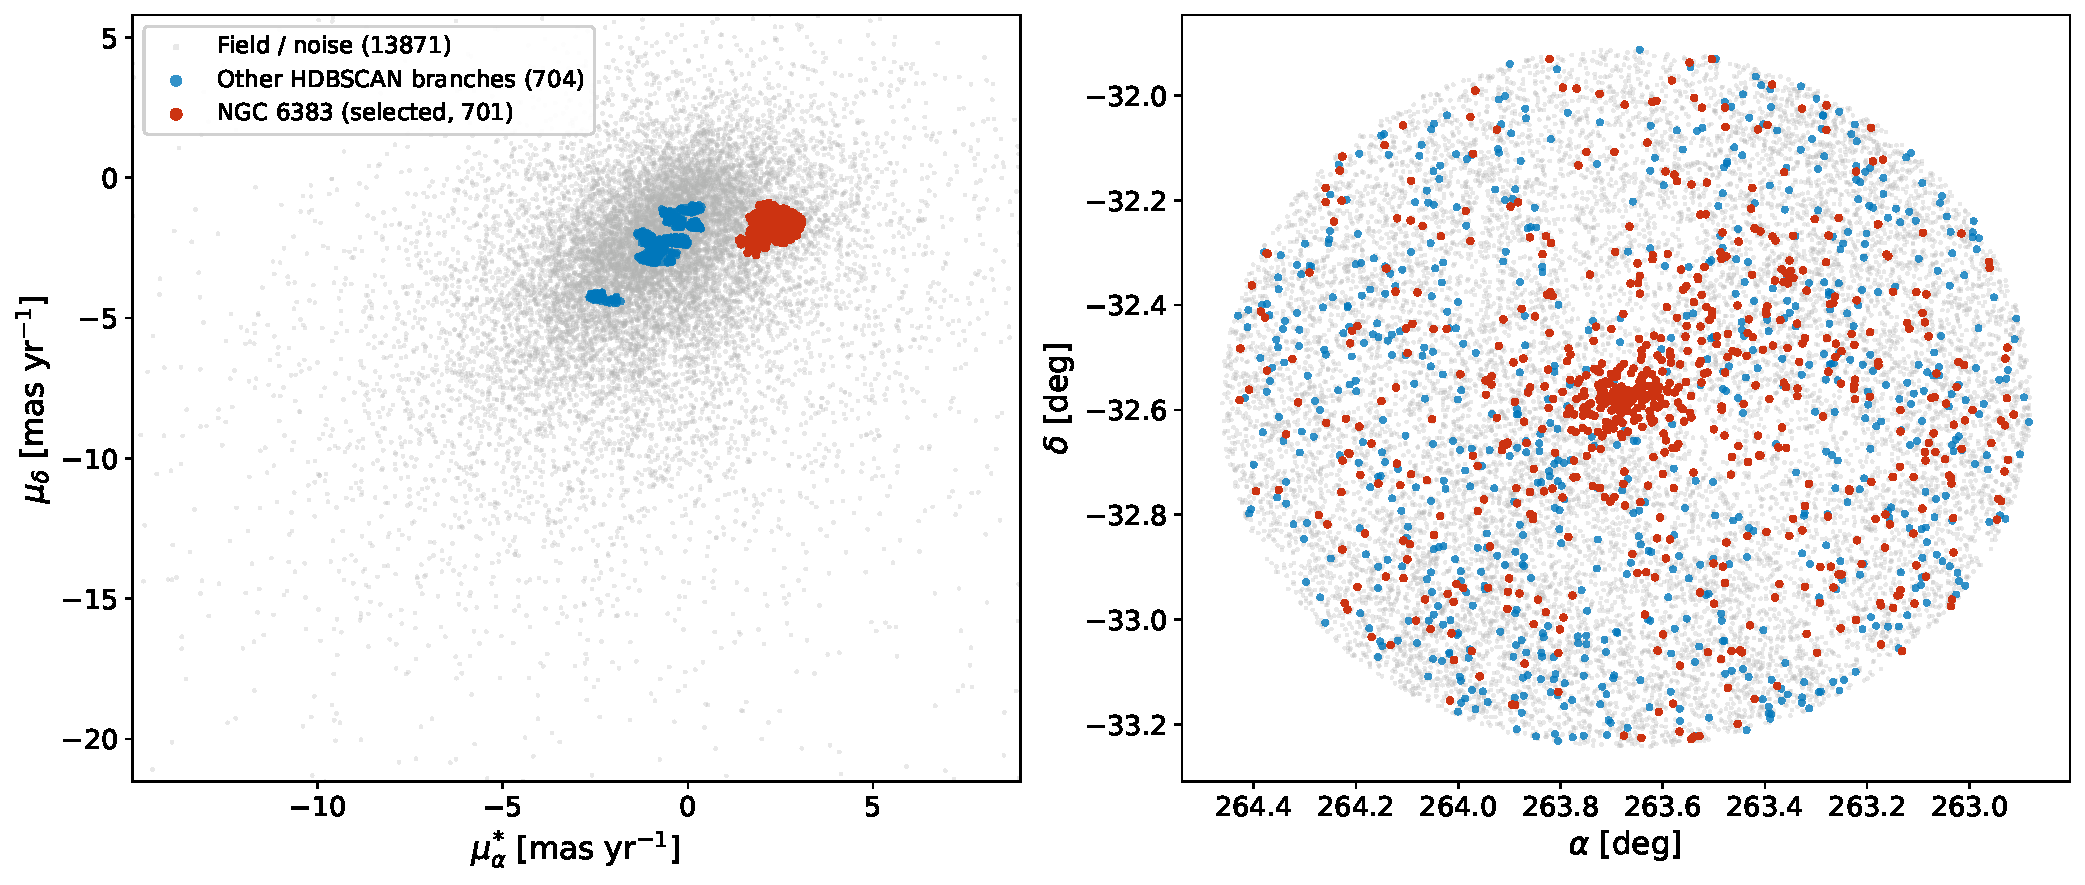
\includegraphics{Figures/pm_radec_overview.pdf}}
\caption{Full HDBSCAN clustering panorama of the $40\,\mathrm{arcmin}$ preprocessed sample ($15276$ sources). \emph{Left:} proper-motion plane $(\mu_{\alpha}^{*},\mu_{\delta})$; \emph{Right:} on-sky distribution in right ascension and declination. Sources are color-coded by their HDBSCAN label: the selected NGC 6383 branch (red), the other HDBSCAN branches (blue), and the field/noise (gray); the legend lists the number of sources in each group. The proper-motion axes are clipped to the $0.5$--$99.5$ percentile range so that the cluster over-density is visible against the broad field distribution. NGC 6383 is a compact, isolated clump in proper motion but overlaps the field on the sky, illustrating that the membership separation is driven by proper motion.}
\label{fig:pm_overview}
\end{figure*}

Figure \ref{fig:plot_pair_trace} shows the joint and marginal distributions of the four ASteCA isochrone-fit parameters together with the likelihood-scatter nuisance term $\sigma$, sampled with the DEMetropolis ensemble (Sect.~\ref{subsec:asteca}). The marginals are single-peaked but only weakly informative: each retains a large fraction of its prior width, and the ensemble does not satisfy the convergence criteria of Sect.~\ref{subsec:cosmic}, so they should be read as a consistency check rather than as sampled posteriors. The off-diagonal panels make the classical CMD-fitting degeneracies explicit: logarithmic age correlates with both visual extinction and distance modulus, so that an older age can be partially compensated by a lower extinction or a smaller distance. Metallicity is the least constrained parameter and remains close to prior-dominated, consistent with the age--metallicity--extinction degeneracy noted in the main text. The intervals quoted for these parameters in the main text and in Table \ref{tab:ngc6383_results} are the marginal spreads of this ensemble; for the reasons just given they are indications of scale rather than calibrated credible widths, as the notes to that table state. $\sigma$ is retained only as a fit nuisance parameter and carries no physical meaning.

\begin{figure*}
\resizebox{\hsize}{!}{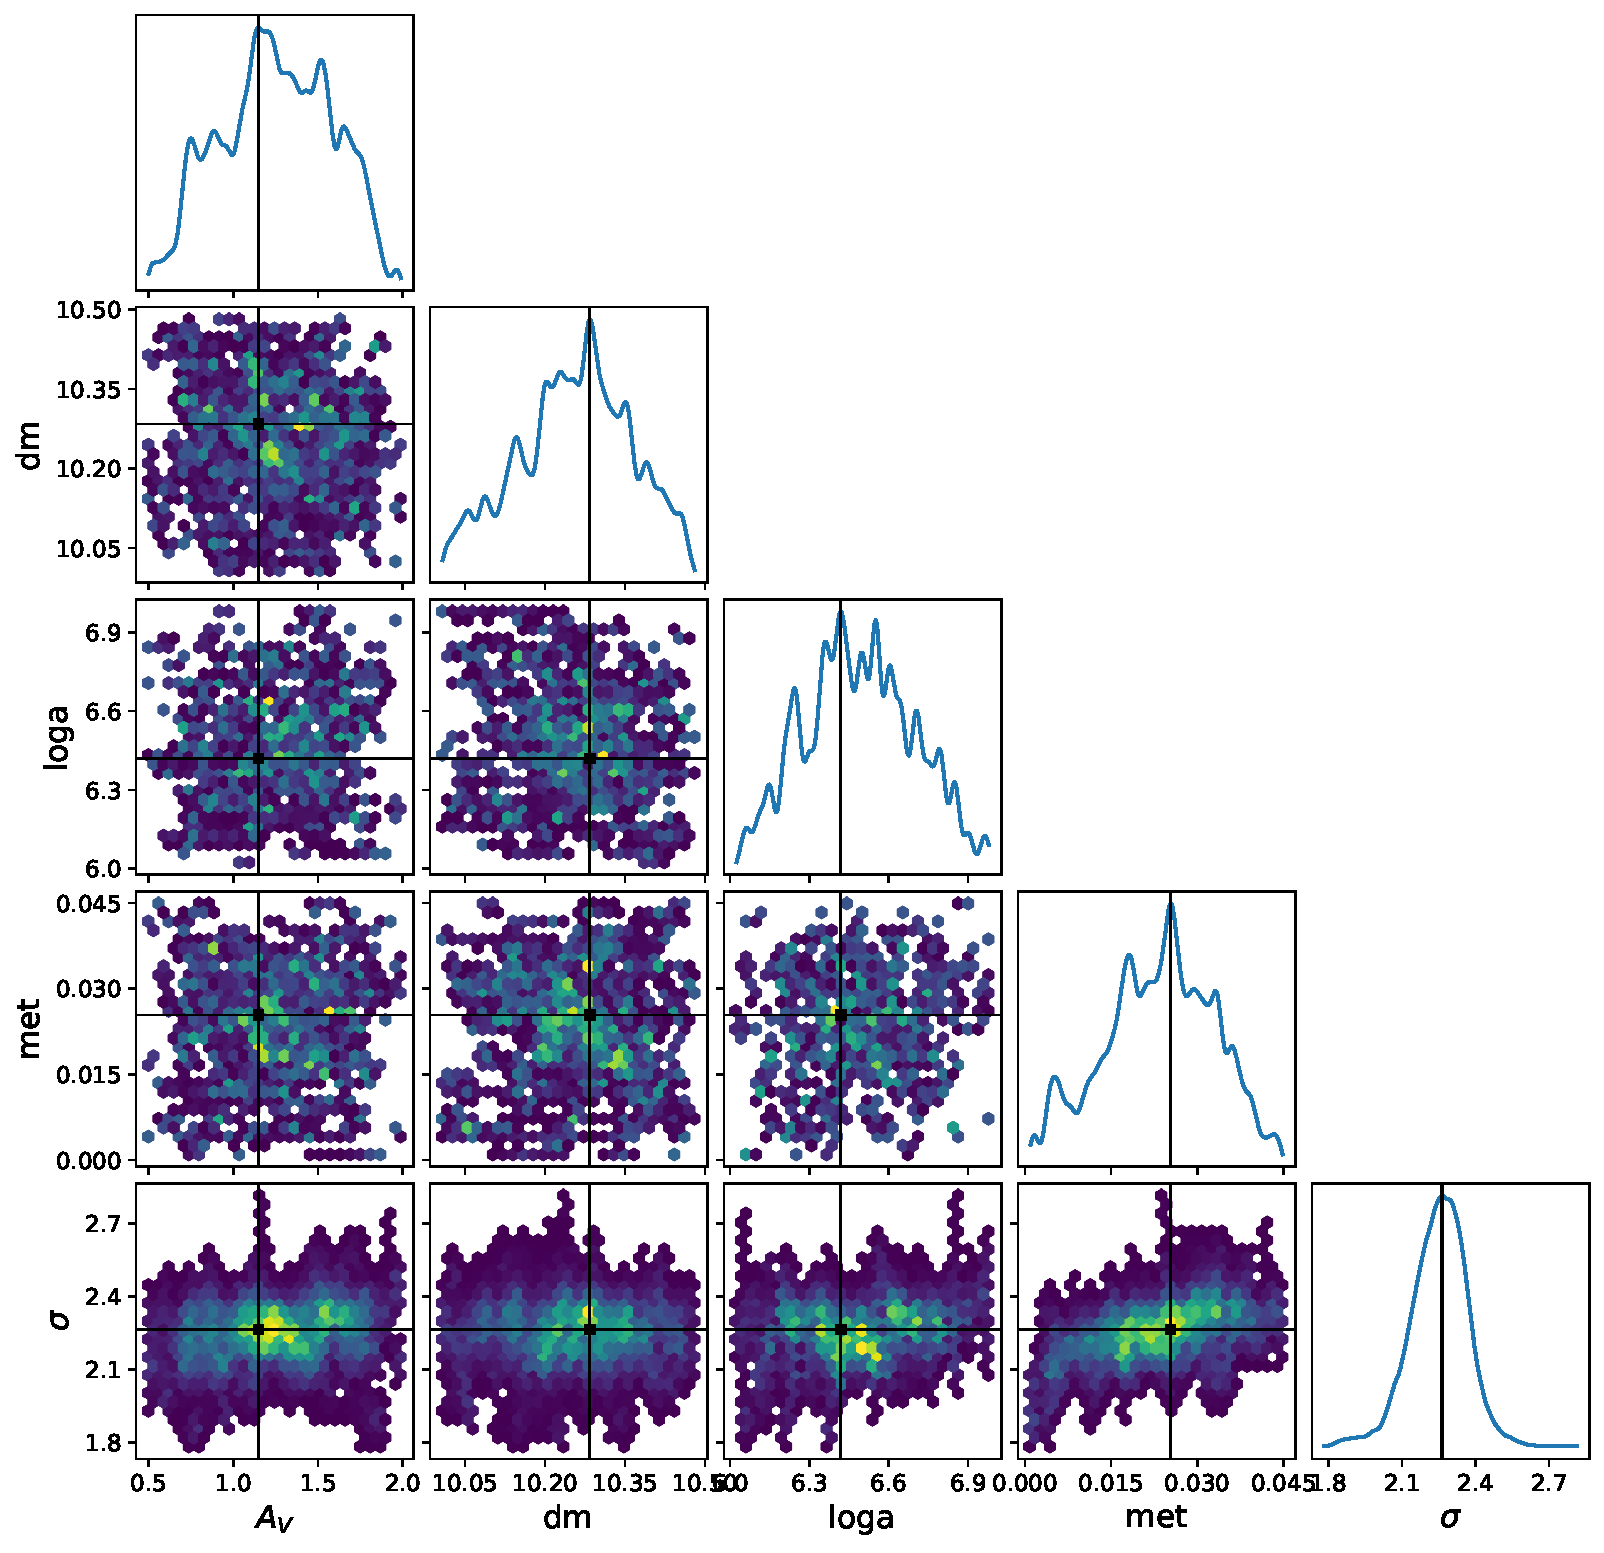
\includegraphics{Figures/plot_pair_trace.pdf}}
\caption{Marginal and joint distributions of the parameters $A_V$ (visual extinction), $dm$ (distance modulus), $loga$ (logarithmic age), $met$ (metallicity), and the nuisance likelihood-scatter parameter $\sigma$, sampled with the DEMetropolis ensemble. The ensemble does not meet the convergence criteria of Sect.~\ref{subsec:cosmic}, so these are a consistency check, not sampled posteriors. The $\sigma$ parameter is the likelihood-scatter term used in the PyMC diagnostic implementation that generated this figure and should not be interpreted as a physical cluster dispersion. The diagonals display the marginal distributions for each parameter (blue curves). The off-diagonal hexbin plots illustrate the joint distributions, highlighting correlations between parameters. Black lines mark the mode of each distribution in all panels; in the off-diagonal panels, the joint mode is additionally marked by a black square.}
\label{fig:plot_pair_trace}
\end{figure*}

\section{Supplementary figures}\label{app:supplementary}

This appendix collects the supplementary figures referenced from the main text: the masses and binarity CMD (Fig. \ref{fig:cmd_mass_binary}); the luminosity function derived from absolute magnitudes (Fig. \ref{fig:lf}); the on-sky distribution of the members with the derived scale radii overlaid on the DSS2-red image (Fig. \ref{fig:real_sky}); the per-star Sagitta PMS-probability, age, and extinction distributions (Fig. \ref{fig:pms_sagitta_stats}); the mass-segregation cumulative distributions for the segregation-time-restricted sample (Fig. \ref{fig:mass_tseg}); and the \textit{Gaia} DR3 radial velocities and their amplitudes (Fig. \ref{fig:radial_velocities}). These figures support, but are not essential to, the results presented in the main text.

\begin{figure}
	\centering
	\resizebox{\hsize}{!}{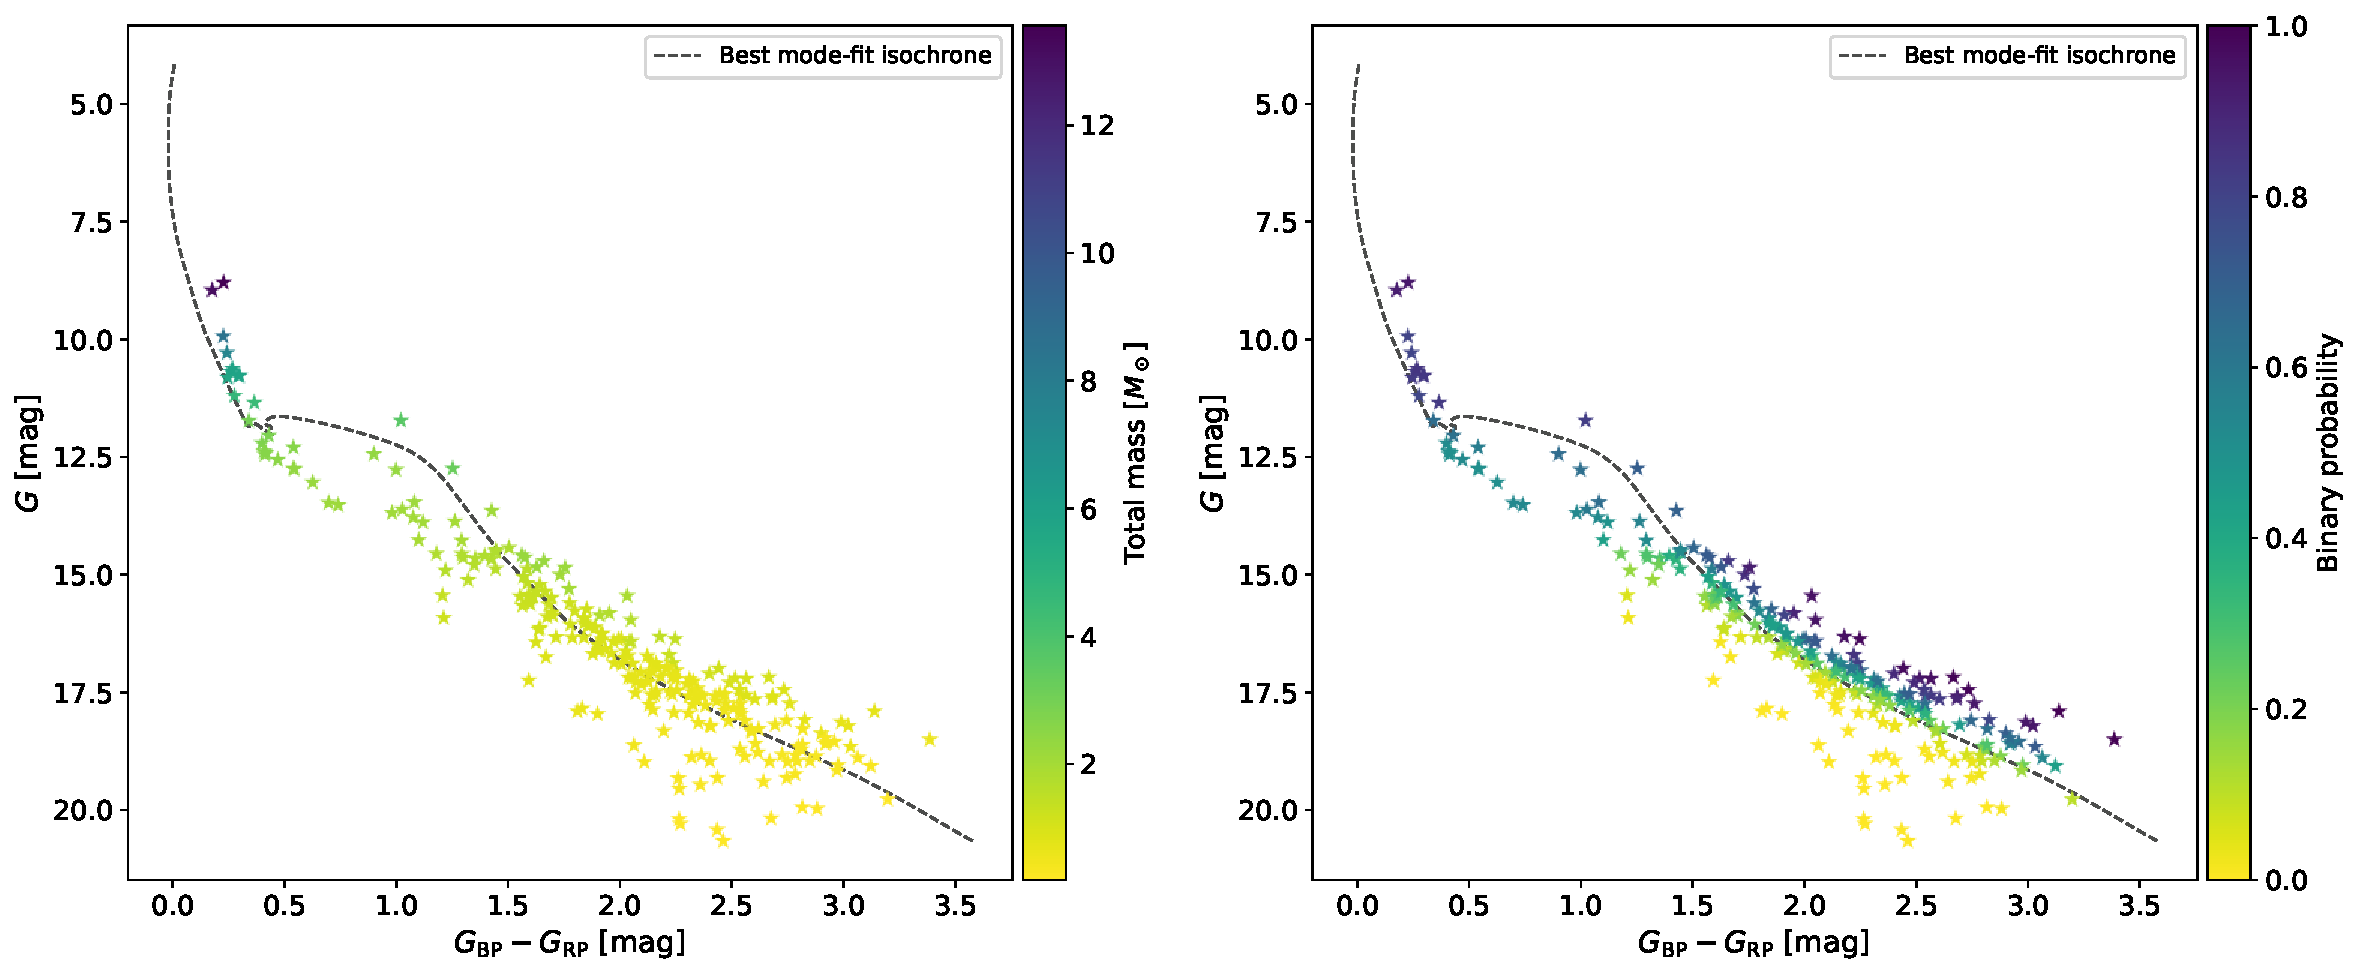
\includegraphics{Figures/ngc6383_mass_binary.pdf}}
	\caption{\emph{Upper panel:} CMD displaying probable members and members of NGC 6383, color-coded by total mass, ranging from lower (yellow) to higher mass (purple). The total mass is calculated as the sum of the two components if the binary probability is greater than $0.7$. \emph{Lower panel:} The same stars as in the upper panel, color-coded by binary probability, from low (yellow) to high (purple). The dark-gray dashed line in both panels is the best mode-fit isochrone.}
	\label{fig:cmd_mass_binary}
\end{figure}

\begin{figure}
	\centering
	\resizebox{\hsize}{!}{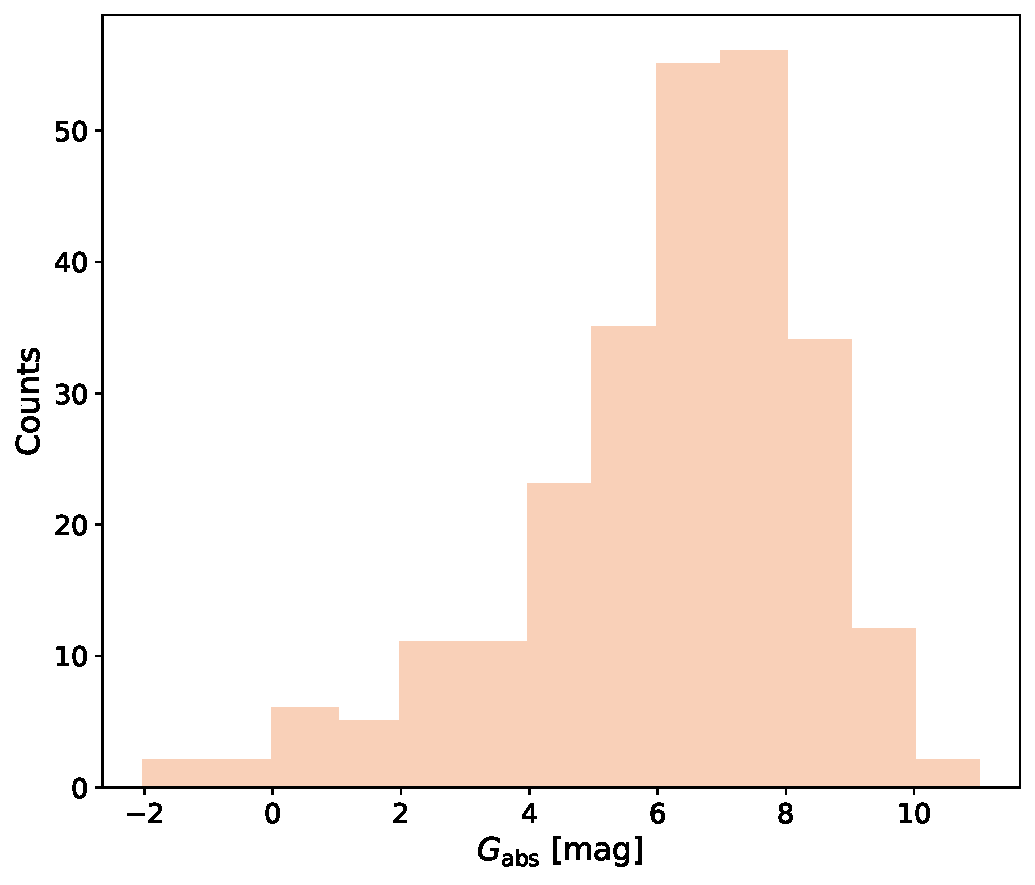
\includegraphics{Figures/luminosity_function.pdf}}
		\caption{Luminosity function of NGC 6383: histogram (orange, hatched) of absolute magnitudes ($ G_{\text{abs}} $) for stars with a membership pseudo-probability of at least $0.6$.}
	\label{fig:lf}
\end{figure}
\begin{figure*}
	\centering
	\resizebox{\hsize}{!}{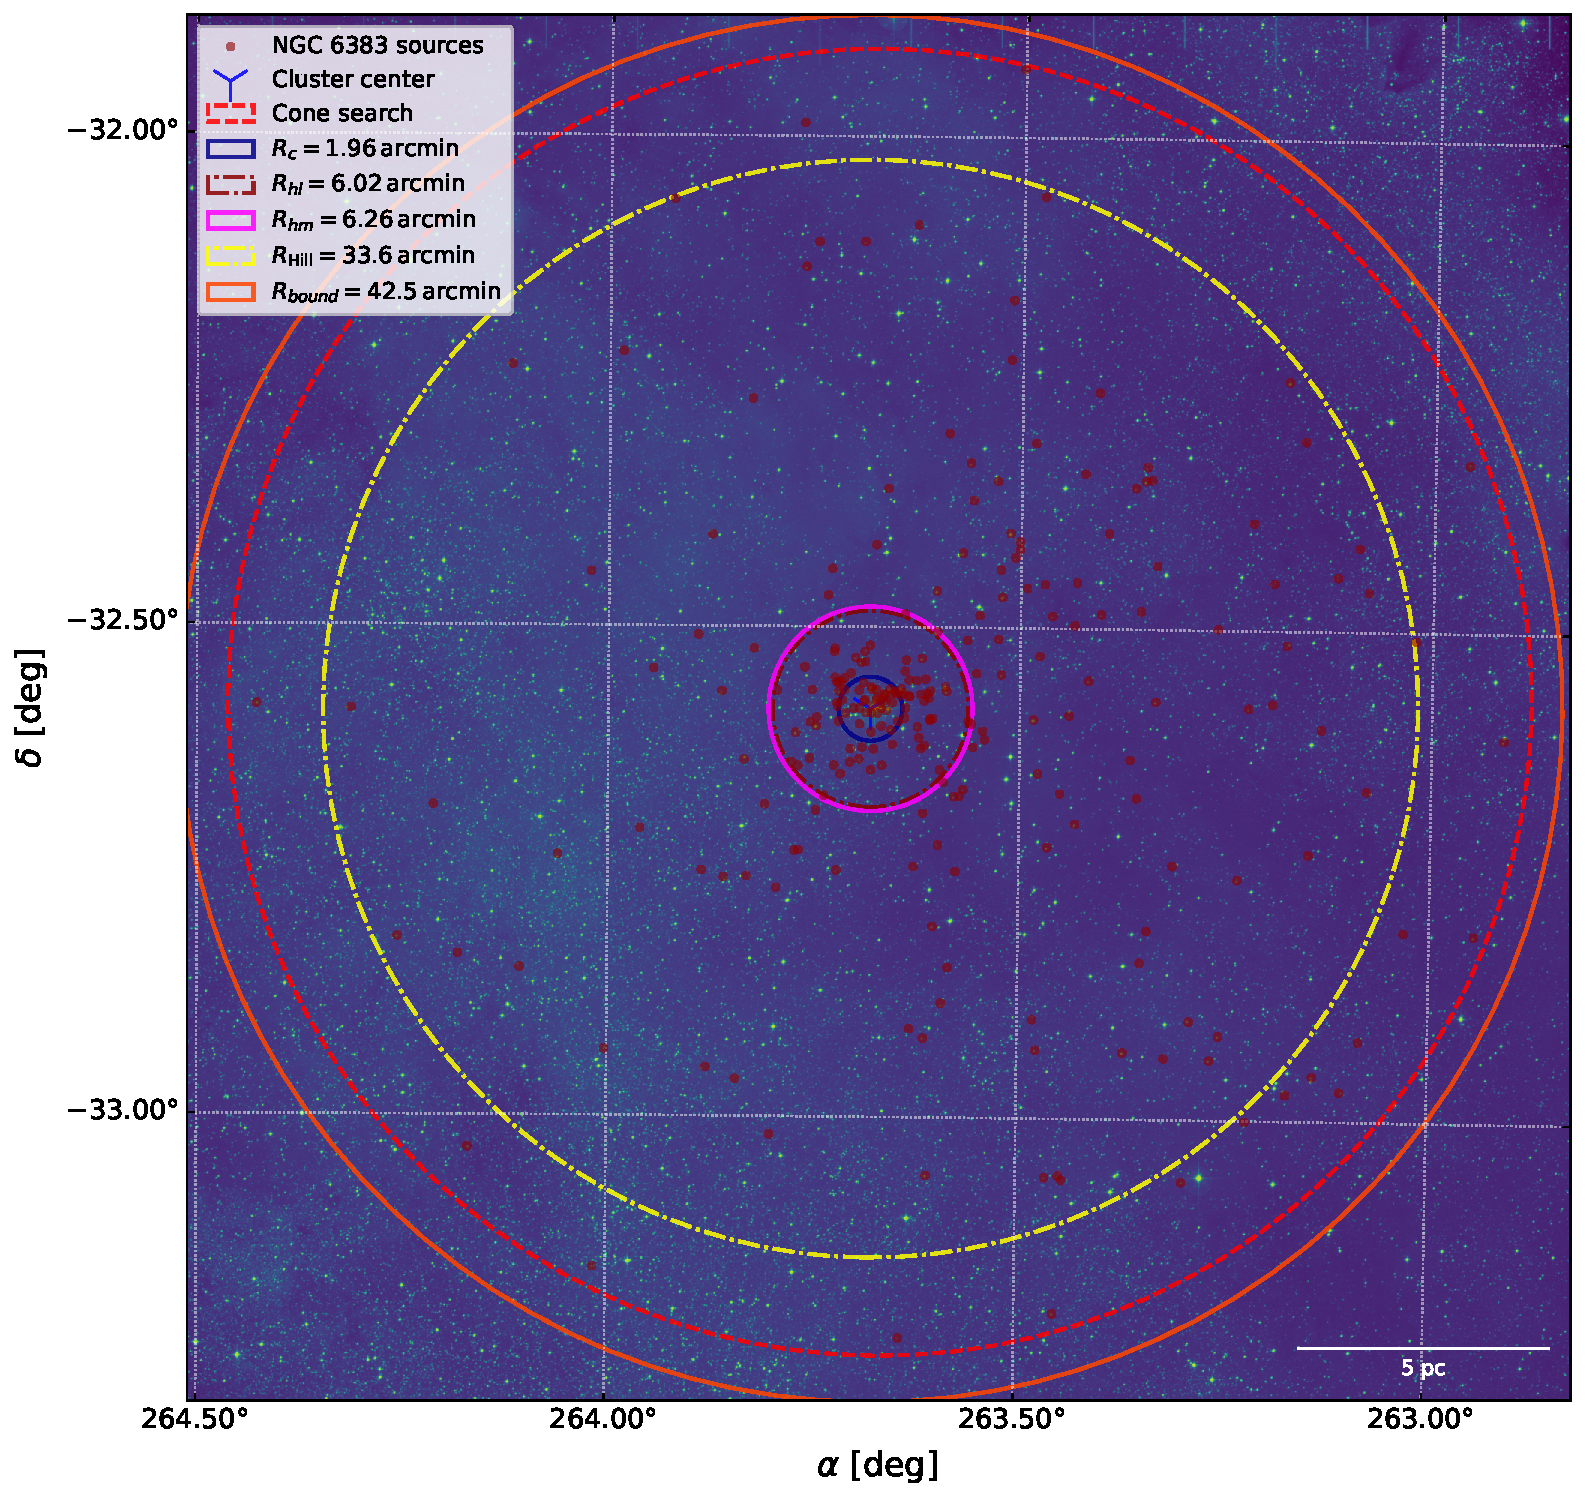
\includegraphics{Figures/real_sky.pdf}}
	\caption{Spatial distribution of probable members and members (dark-red dots) overlaid on a DSS2-red background image (shown in false color), centered on the derived cluster center marked by a blue marker. The circles are the $40\,\mathrm{arcmin}$ cone-search radius and, in increasing order of size, the fitted or derived scale radii $R_c$, $R_{\mathrm{hl}}$, $R_{\mathrm{hm}}$, $R_{\mathrm{Hill}}$, and $R_{\mathrm{bound}}$, whose values are given in the legend. The adopted King outer radius ($R_t = 54\,\mathrm{arcmin}$, Appendix~\ref{app:window}, Fig.~\ref{fig:king70}) lies just outside the displayed field and is not drawn.}
	\label{fig:real_sky}
\end{figure*}

\begin{figure}
	\centering
	\resizebox{\hsize}{!}{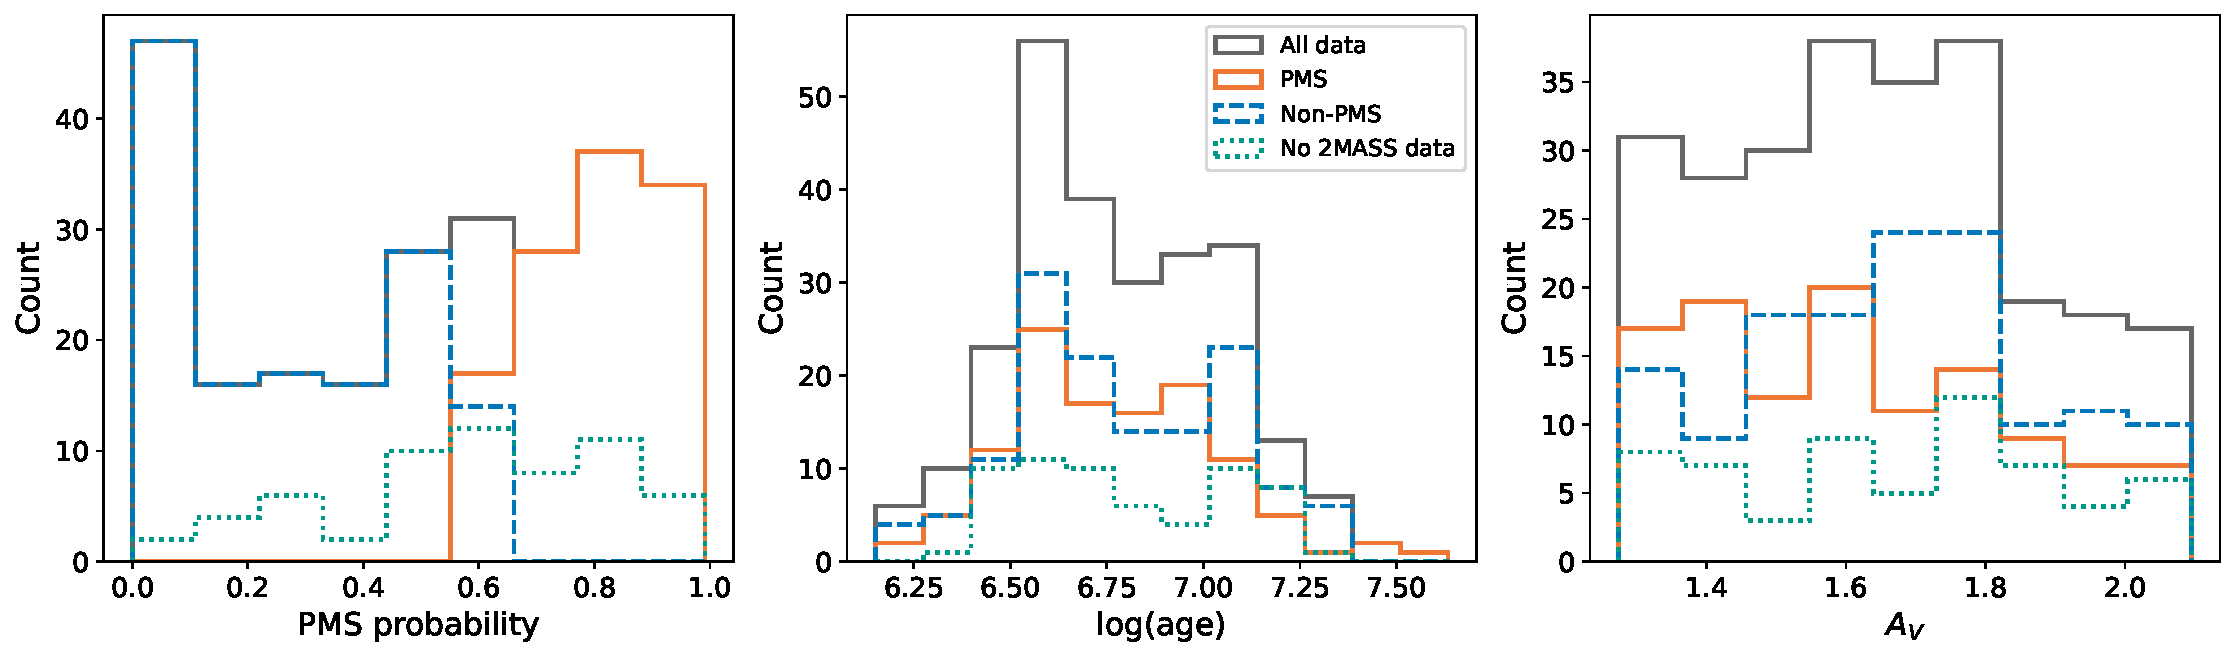
\includegraphics{Figures/pms_stats.pdf}}
	\caption{Histograms of the parameters obtained with Sagitta for the NGC 6383 reference sample ($\tilde{p}\geq0.6$), including all data (gray solid), sources with a PMS probability of at least $60\%$ (orange solid), sources with a PMS probability under $60\%$ (blue dashed), and stars with missing 2MASS data (green dotted); the legend in the middle panel applies to all panels. The upper panel shows the distribution of PMS probability values, indicating the likelihood of stars being PMS; the middle panel presents the distribution of logarithmic age values, illustrating the range and frequency of stellar ages within the cluster; and the lower panel displays the distribution of visual extinction values ($A_V$), representing the amount of dust extinction affecting the observed stars.}
	\label{fig:pms_sagitta_stats}
\end{figure}

\begin{figure*}
	\centering
	\resizebox{\hsize}{!}{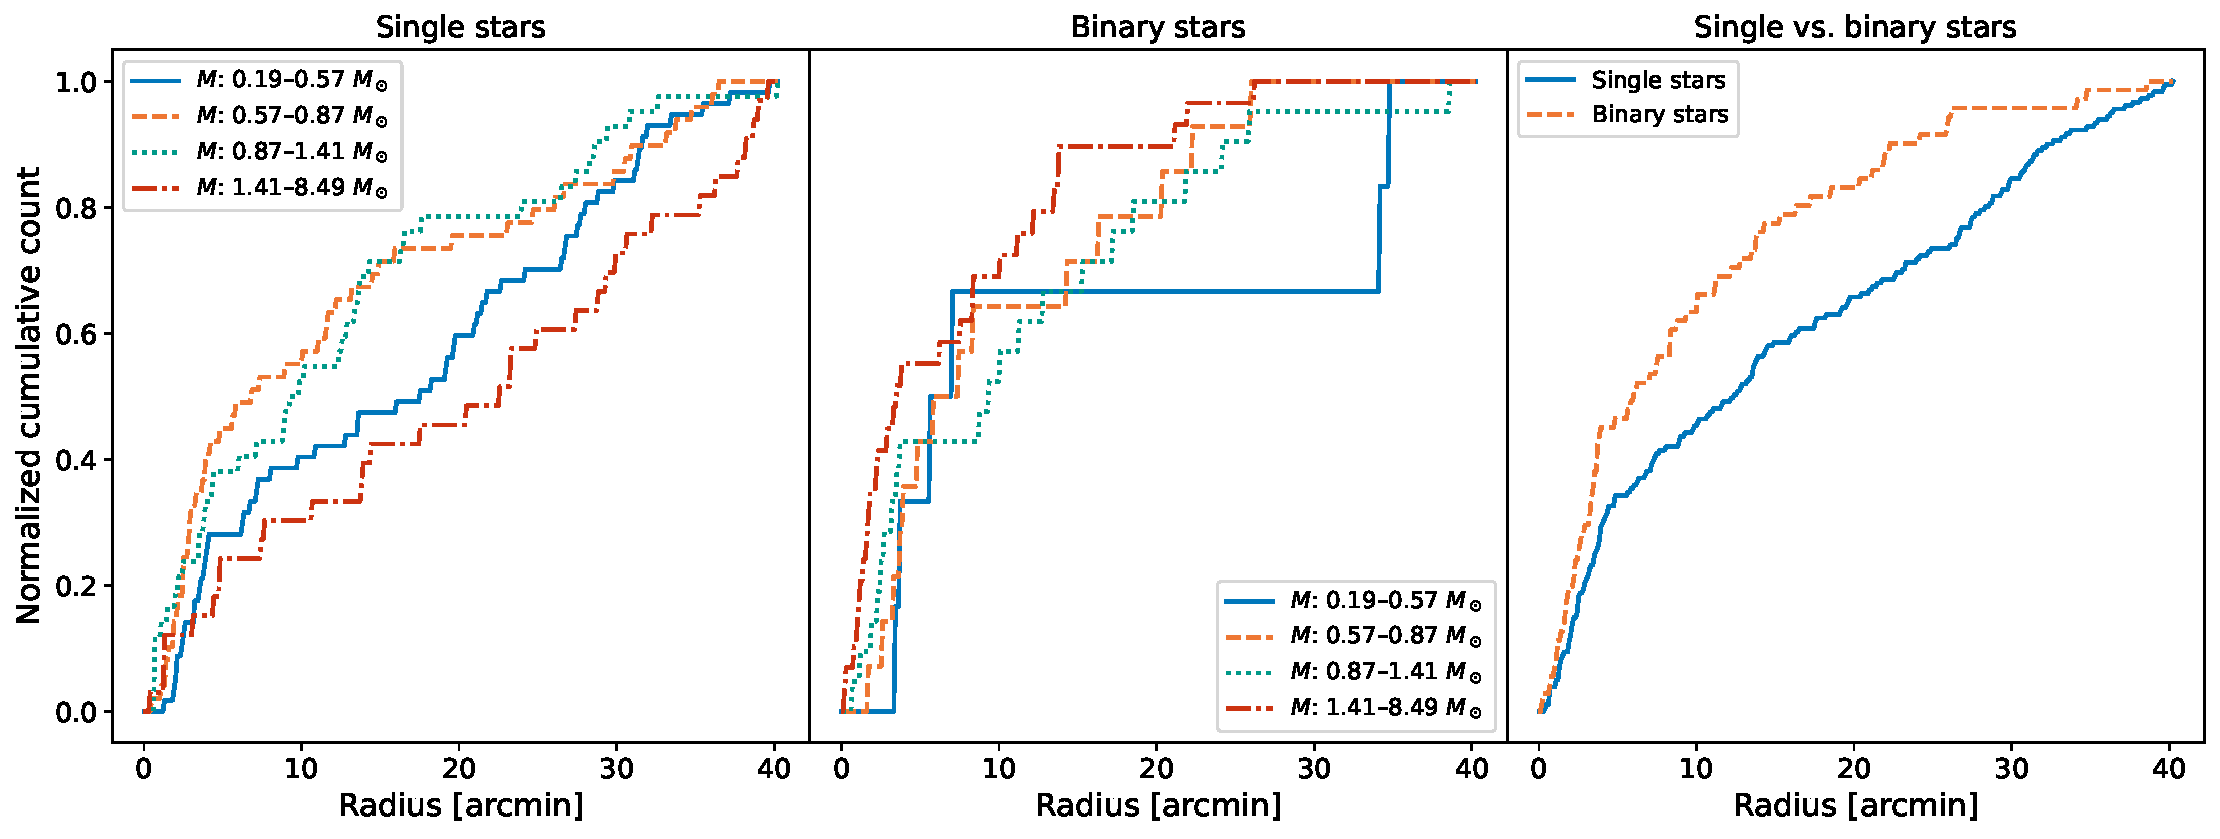
\includegraphics{Figures/cumulative_by_mass_and_type_mseg.pdf}}
	\caption{Same as Fig. \ref{fig:mass_seg}, but restricted to stars whose segregation time exceeds the cluster age ($t_{\mathrm{seg}}(m)>3.53\,\mathrm{Myr}$, i.e. $M < 9.1\,M_\odot$; Sect.~\ref{subsec:lum_mass_dyn}); the mass quartiles are recomputed for this truncated sample (uppermost quartile $1.41$--$8.49\,M_\odot$).}
	\label{fig:mass_tseg}
\end{figure*}

\begin{figure}
	\centering
	\resizebox{\hsize}{!}{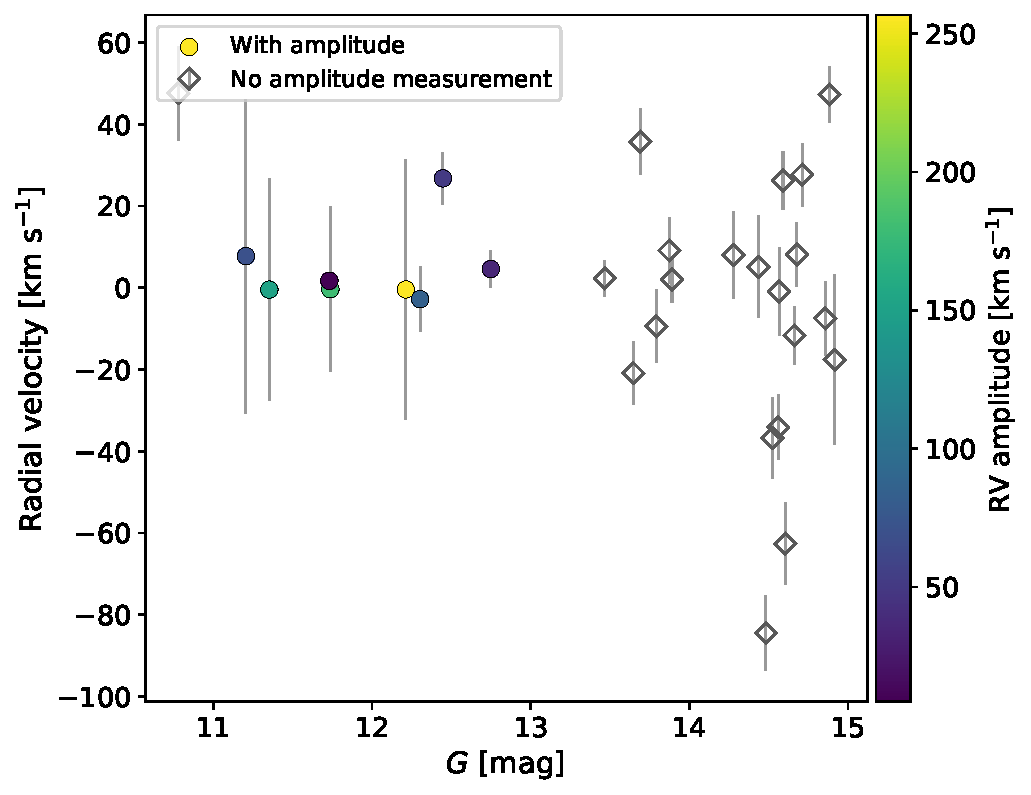
\includegraphics{Figures/radial_velocity_amplitude.pdf}}
	\caption{Radial velocity versus $G$ magnitude for the 29 reference-sample sources with \textit{Gaia} DR3 radial velocities. Filled circles have DR3 amplitude measurements (\texttt{rv\_amplitude\_robust}, which reflects the total amplitude in the radial-velocity time series following outlier removal) and are color-coded by amplitude (viridis color bar); open gray diamonds lack amplitude measurements. Vertical bars show the radial-velocity uncertainties.}
	\label{fig:radial_velocities}
\end{figure}

\clearpage
\section{Search-window sensitivity of the derived parameters}\label{app:window}

This appendix complements the membership-recovery counts of Table \ref{tab:cone_robustness} by listing, side by side, the astrometric and structural parameters recovered at each input cone-search radius. Only the membership, astrometric, and King-structural quantities were recomputed for the wider fields; the photometric quantities (ages, masses, and the mass-segregation diagnostics) remain tied to the $40\,\mathrm{arcmin}$ reference catalog and are not repeated per radius. As discussed in Sect.~\ref{subsec:member_results}, the catalog-level astrometry is stable across radii, whereas the structural parameters and the outer-membership counts drift once the automated branch selection becomes field-window dependent (at $60$ and $70\,\mathrm{arcmin}$).

The $70\,\mathrm{arcmin}$ window provides the adopted King outer radius (Sect.~\ref{subsec:structural}). The probability that $R_t$ exceeds the extraction window decreases from $51\%$ at $40\,\mathrm{arcmin}$ to $40\%$ and $13\%$ at $50$ and $60\,\mathrm{arcmin}$ (at $70\,\mathrm{arcmin}$ it vanishes by construction, since the prior support ends at $1.5\,T_{\mathrm{max}}=63.7\,\mathrm{arcmin}$), and Fig.~\ref{fig:king70} shows that only this window reaches a well-defined background annulus beyond the cluster, with fitted background $b=0.020^{+0.006}_{-0.010}$ and central density $k=8.42\pm0.17$ stars per square arcminute. All $R_t$ posteriors, including the adopted one, are truncated from above by the physically motivated $1.5\,T_{\mathrm{max}}$ prior bound and remain conditional on it; the shift under a relaxed bound is quantified in Sect.~\ref{subsec:structural}. The background of this membership-selected sample measures the residual contamination level of the selection, not the raw field density. The core radius and central density of the $70\,\mathrm{arcmin}$ fit are contamination-biased (Sect.~\ref{subsec:member_results}) and are not adopted. Adopting $R_t$ from a fit whose $R_c$ we reject requires an argument, and it is one of sensitivity rather than of trust: the additional sources admitted at $70\,\mathrm{arcmin}$ are concentrated at small radii ($114$ of the $376$ added lie inside the $40\,\mathrm{arcmin}$ footprint), where they raise the central density and pull $R_c$ down, whereas $R_t$ is set by where the profile meets the fitted background annulus, which those inner additions do not move. The two parameters are therefore not equally exposed to the same contamination. This does not make $R_t$ immune, and we note the consequence explicitly: the concentration parameter $C$ combines posteriors from two fits on two samples and should be read as such.

\begin{figure}
	\centering
	\resizebox{\hsize}{!}{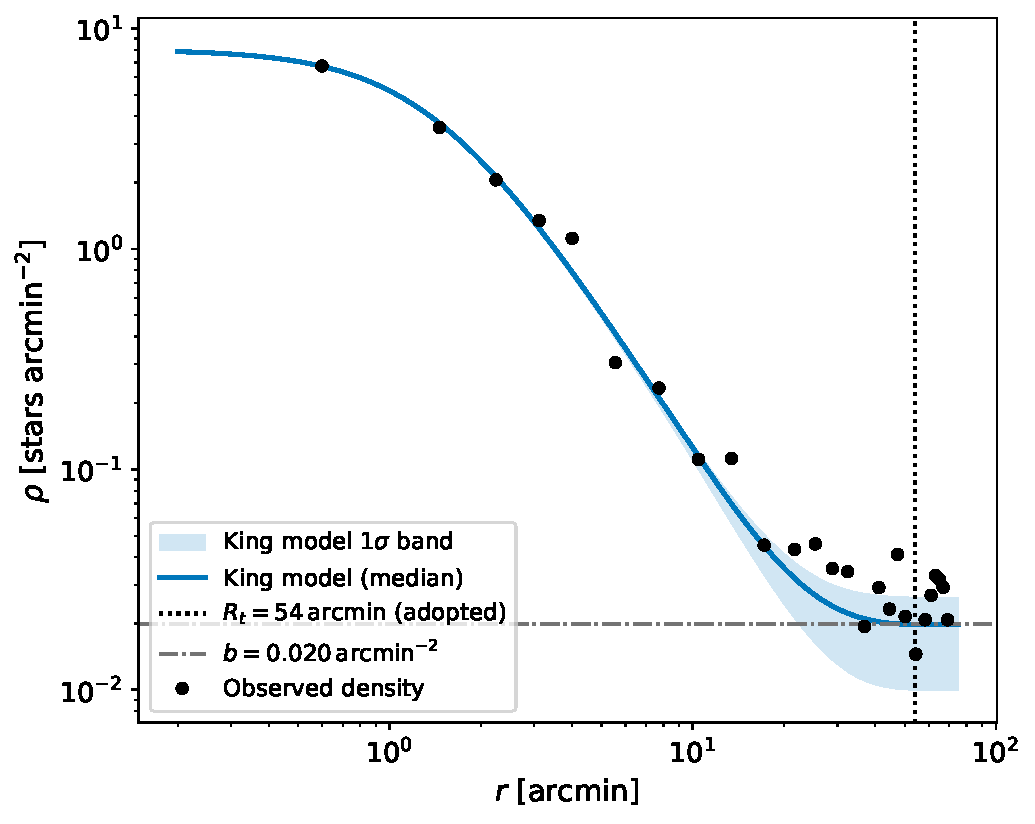
\includegraphics{Figures/king_profile_cone70.pdf}}
	\caption{Radial density profile of the $70\,\mathrm{arcmin}$ extraction ($N=628$, $\tilde{p}\geq0.6$) with the King model at the posterior median (blue solid line) and its 16--84\% posterior band (blue shading). The black dotted vertical line marks the adopted King outer radius ($R_t = 54\,\mathrm{arcmin}$) and the gray dash-dotted horizontal line the fitted background level $b$. Unlike the $40\,\mathrm{arcmin}$ fit (Fig.~\ref{fig:king}), this window contains a genuine background annulus beyond the cluster, so the outer radius is background-constrained; the higher central density and smaller core radius reflect the additional field contamination of this sample and are not adopted.}
	\label{fig:king70}
\end{figure}

\begin{table*}
		\caption{Robustness of the membership recovery against the input cone-search radius. The $40\,\mathrm{arcmin}$ row is the production catalog used for the adopted cluster parameters, while the $50$--$70\,\mathrm{arcmin}$ rows are wider-field robustness checks. Each run used the same preprocessing, the same proper-motion-only HDBSCAN feature space, the same pseudo-probability construction as in Sect. \ref{subsubsec:membership}, and the same parallax-mode sigma clipping. The algorithm-selected branch is the branch selected by the generic sweep rule, while the NGC-like branch is the final HDBSCAN label closest to the reference proper motion of NGC 6383, $(\mu_{\alpha*},\mu_{\delta})=(2.542,-1.713)\,\mathrm{mas\,yr^{-1}}$.}
	\centering
	\begin{tabular}{ccccccccc}
		\hline
		Radius & Preprocessed & Best $m_\mathrm{cl}$ & Algorithm & NGC-like & NGC branch & $\tilde{p}>0.5$ & $\tilde{p}\geq0.6$ & Common with \\
		(arcmin) & sources &  & label & label & size & after clip & reference sample & adopted 254 \\
		\hline
		40 & 15276 & 43  & 0  & 0  & 701 & 321 & 254 & 254 \\
		50 & 23844 & 18  & 28 & 28 & 767 & 355 & 236 & 203 \\
		60 & 33309 & 143 & 1  & 0  & 696 & 476 & 443 & 242 \\
		70 & 44438 & 177 & 1  & 0  & 798 & 650 & 628 & 252 \\
		\hline
	\end{tabular}
	\label{tab:cone_robustness}
\end{table*}

\begin{table*}
	\caption{Astrometric and King-structural parameters recovered at each input cone-search radius. The $40\,\mathrm{arcmin}$ row is the adopted production fit; the $50$--$70\,\mathrm{arcmin}$ rows use the same King priors applied to the wider-field reference samples. $N$ is the number of reference-sample candidates ($\tilde{p}\geq0.6$). The mean parallax $\bar{\varpi}$ is quoted with the $1\sigma$ dispersion of the subsample with $\delta\varpi/\varpi<0.1$; the proper-motion means carry the $1\sigma$ member dispersions. The core radius $R_c$, King outer radius $R_t$, and concentration $C=\log_{10}(R_t/R_c)$ are the posterior medians with 16--84\% credible intervals of the King fit; $P(R_t>W)$ is the posterior probability that $R_t$ exceeds the extraction window. Ages, masses, and mass segregation were not recomputed per radius (see text).}
	\centering
	\begin{tabular}{ccccccccc}
		\hline
		Radius & $N$ & $\bar{\varpi}$ & $\mu_{\alpha*}$ & $\mu_{\delta}$ & $R_c$ & $R_t$ & $C$ & $P(R_t>W)$ \\
		(arcmin) & ($\tilde{p}\geq0.6$) & (mas) & (mas\,yr$^{-1}$) & (mas\,yr$^{-1}$) & (arcmin) & (arcmin) &  & (\%) \\
		\hline
		40 & 254 & $0.908\pm0.046$ & $2.542\pm0.152$ & $-1.713\pm0.138$ & $1.96^{+0.19}_{-0.16}$ & $40^{+16}_{-17}$ & $1.32^{+0.16}_{-0.27}$ & 51 \\
		50 & 236 & $0.906\pm0.044$ & $2.544\pm0.133$ & $-1.711\pm0.127$ & $1.90^{+0.15}_{-0.13}$ & $46^{+12}_{-16}$ & $1.39^{+0.11}_{-0.20}$ & 40 \\
		60 & 443 & $0.916\pm0.051$ & $2.455\pm0.239$ & $-1.693\pm0.159$ & $1.36^{+0.10}_{-0.09}$ & $47^{+12}_{-16}$ & $1.54^{+0.10}_{-0.19}$ & 13 \\
		70 & 628 & $0.915\pm0.057$ & $2.383\pm0.279$ & $-1.680\pm0.163$ & $1.38^{+0.04}_{-0.04}$ & $54^{+7}_{-11}$  & $1.59^{+0.06}_{-0.11}$ & 0 \\
		\hline
	\end{tabular}
	\label{tab:cone_params}
\end{table*}

\end{appendix}
\end{document}
